% Options for packages loaded elsewhere
\PassOptionsToPackage{unicode}{hyperref}
\PassOptionsToPackage{hyphens}{url}
\PassOptionsToPackage{dvipsnames,svgnames,x11names}{xcolor}
%
\documentclass[
  11pt,
  a4paper,
  DIV=11,
  numbers=noendperiod]{scrartcl}

\usepackage{amsmath,amssymb}
\usepackage{iftex}
\ifPDFTeX
  \usepackage[T1]{fontenc}
  \usepackage[utf8]{inputenc}
  \usepackage{textcomp} % provide euro and other symbols
\else % if luatex or xetex
  \usepackage{unicode-math}
  \defaultfontfeatures{Scale=MatchLowercase}
  \defaultfontfeatures[\rmfamily]{Ligatures=TeX,Scale=1}
\fi
\usepackage{lmodern}
\ifPDFTeX\else  
    % xetex/luatex font selection
\fi
% Use upquote if available, for straight quotes in verbatim environments
\IfFileExists{upquote.sty}{\usepackage{upquote}}{}
\IfFileExists{microtype.sty}{% use microtype if available
  \usepackage[]{microtype}
  \UseMicrotypeSet[protrusion]{basicmath} % disable protrusion for tt fonts
}{}
\makeatletter
\@ifundefined{KOMAClassName}{% if non-KOMA class
  \IfFileExists{parskip.sty}{%
    \usepackage{parskip}
  }{% else
    \setlength{\parindent}{0pt}
    \setlength{\parskip}{6pt plus 2pt minus 1pt}}
}{% if KOMA class
  \KOMAoptions{parskip=half}}
\makeatother
\usepackage{xcolor}
\usepackage[lmargin=2cm,rmargin=2cm,tmargin=2cm,bmargin=2cm]{geometry}
\setlength{\emergencystretch}{3em} % prevent overfull lines
\setcounter{secnumdepth}{-\maxdimen} % remove section numbering
% Make \paragraph and \subparagraph free-standing
\ifx\paragraph\undefined\else
  \let\oldparagraph\paragraph
  \renewcommand{\paragraph}[1]{\oldparagraph{#1}\mbox{}}
\fi
\ifx\subparagraph\undefined\else
  \let\oldsubparagraph\subparagraph
  \renewcommand{\subparagraph}[1]{\oldsubparagraph{#1}\mbox{}}
\fi

\usepackage{color}
\usepackage{fancyvrb}
\newcommand{\VerbBar}{|}
\newcommand{\VERB}{\Verb[commandchars=\\\{\}]}
\DefineVerbatimEnvironment{Highlighting}{Verbatim}{commandchars=\\\{\}}
% Add ',fontsize=\small' for more characters per line
\usepackage{framed}
\definecolor{shadecolor}{RGB}{241,243,245}
\newenvironment{Shaded}{\begin{snugshade}}{\end{snugshade}}
\newcommand{\AlertTok}[1]{\textcolor[rgb]{0.68,0.00,0.00}{#1}}
\newcommand{\AnnotationTok}[1]{\textcolor[rgb]{0.37,0.37,0.37}{#1}}
\newcommand{\AttributeTok}[1]{\textcolor[rgb]{0.40,0.45,0.13}{#1}}
\newcommand{\BaseNTok}[1]{\textcolor[rgb]{0.68,0.00,0.00}{#1}}
\newcommand{\BuiltInTok}[1]{\textcolor[rgb]{0.00,0.23,0.31}{#1}}
\newcommand{\CharTok}[1]{\textcolor[rgb]{0.13,0.47,0.30}{#1}}
\newcommand{\CommentTok}[1]{\textcolor[rgb]{0.37,0.37,0.37}{#1}}
\newcommand{\CommentVarTok}[1]{\textcolor[rgb]{0.37,0.37,0.37}{\textit{#1}}}
\newcommand{\ConstantTok}[1]{\textcolor[rgb]{0.56,0.35,0.01}{#1}}
\newcommand{\ControlFlowTok}[1]{\textcolor[rgb]{0.00,0.23,0.31}{#1}}
\newcommand{\DataTypeTok}[1]{\textcolor[rgb]{0.68,0.00,0.00}{#1}}
\newcommand{\DecValTok}[1]{\textcolor[rgb]{0.68,0.00,0.00}{#1}}
\newcommand{\DocumentationTok}[1]{\textcolor[rgb]{0.37,0.37,0.37}{\textit{#1}}}
\newcommand{\ErrorTok}[1]{\textcolor[rgb]{0.68,0.00,0.00}{#1}}
\newcommand{\ExtensionTok}[1]{\textcolor[rgb]{0.00,0.23,0.31}{#1}}
\newcommand{\FloatTok}[1]{\textcolor[rgb]{0.68,0.00,0.00}{#1}}
\newcommand{\FunctionTok}[1]{\textcolor[rgb]{0.28,0.35,0.67}{#1}}
\newcommand{\ImportTok}[1]{\textcolor[rgb]{0.00,0.46,0.62}{#1}}
\newcommand{\InformationTok}[1]{\textcolor[rgb]{0.37,0.37,0.37}{#1}}
\newcommand{\KeywordTok}[1]{\textcolor[rgb]{0.00,0.23,0.31}{#1}}
\newcommand{\NormalTok}[1]{\textcolor[rgb]{0.00,0.23,0.31}{#1}}
\newcommand{\OperatorTok}[1]{\textcolor[rgb]{0.37,0.37,0.37}{#1}}
\newcommand{\OtherTok}[1]{\textcolor[rgb]{0.00,0.23,0.31}{#1}}
\newcommand{\PreprocessorTok}[1]{\textcolor[rgb]{0.68,0.00,0.00}{#1}}
\newcommand{\RegionMarkerTok}[1]{\textcolor[rgb]{0.00,0.23,0.31}{#1}}
\newcommand{\SpecialCharTok}[1]{\textcolor[rgb]{0.37,0.37,0.37}{#1}}
\newcommand{\SpecialStringTok}[1]{\textcolor[rgb]{0.13,0.47,0.30}{#1}}
\newcommand{\StringTok}[1]{\textcolor[rgb]{0.13,0.47,0.30}{#1}}
\newcommand{\VariableTok}[1]{\textcolor[rgb]{0.07,0.07,0.07}{#1}}
\newcommand{\VerbatimStringTok}[1]{\textcolor[rgb]{0.13,0.47,0.30}{#1}}
\newcommand{\WarningTok}[1]{\textcolor[rgb]{0.37,0.37,0.37}{\textit{#1}}}

\providecommand{\tightlist}{%
  \setlength{\itemsep}{0pt}\setlength{\parskip}{0pt}}\usepackage{longtable,booktabs,array}
\usepackage{calc} % for calculating minipage widths
% Correct order of tables after \paragraph or \subparagraph
\usepackage{etoolbox}
\makeatletter
\patchcmd\longtable{\par}{\if@noskipsec\mbox{}\fi\par}{}{}
\makeatother
% Allow footnotes in longtable head/foot
\IfFileExists{footnotehyper.sty}{\usepackage{footnotehyper}}{\usepackage{footnote}}
\makesavenoteenv{longtable}
\usepackage{graphicx}
\makeatletter
\def\maxwidth{\ifdim\Gin@nat@width>\linewidth\linewidth\else\Gin@nat@width\fi}
\def\maxheight{\ifdim\Gin@nat@height>\textheight\textheight\else\Gin@nat@height\fi}
\makeatother
% Scale images if necessary, so that they will not overflow the page
% margins by default, and it is still possible to overwrite the defaults
% using explicit options in \includegraphics[width, height, ...]{}
\setkeys{Gin}{width=\maxwidth,height=\maxheight,keepaspectratio}
% Set default figure placement to htbp
\makeatletter
\def\fps@figure{htbp}
\makeatother

\KOMAoption{captions}{tableheading}
\makeatletter
\@ifpackageloaded{caption}{}{\usepackage{caption}}
\AtBeginDocument{%
\ifdefined\contentsname
  \renewcommand*\contentsname{Table of contents}
\else
  \newcommand\contentsname{Table of contents}
\fi
\ifdefined\listfigurename
  \renewcommand*\listfigurename{List of Figures}
\else
  \newcommand\listfigurename{List of Figures}
\fi
\ifdefined\listtablename
  \renewcommand*\listtablename{List of Tables}
\else
  \newcommand\listtablename{List of Tables}
\fi
\ifdefined\figurename
  \renewcommand*\figurename{Figure}
\else
  \newcommand\figurename{Figure}
\fi
\ifdefined\tablename
  \renewcommand*\tablename{Table}
\else
  \newcommand\tablename{Table}
\fi
}
\@ifpackageloaded{float}{}{\usepackage{float}}
\floatstyle{ruled}
\@ifundefined{c@chapter}{\newfloat{codelisting}{h}{lop}}{\newfloat{codelisting}{h}{lop}[chapter]}
\floatname{codelisting}{Listing}
\newcommand*\listoflistings{\listof{codelisting}{List of Listings}}
\makeatother
\makeatletter
\makeatother
\makeatletter
\@ifpackageloaded{caption}{}{\usepackage{caption}}
\@ifpackageloaded{subcaption}{}{\usepackage{subcaption}}
\makeatother
\ifLuaTeX
  \usepackage{selnolig}  % disable illegal ligatures
\fi
\usepackage{bookmark}

\IfFileExists{xurl.sty}{\usepackage{xurl}}{} % add URL line breaks if available
\urlstyle{same} % disable monospaced font for URLs
\hypersetup{
  pdftitle={STOP COMPLAINING, IT SOLVES NOTHING.},
  colorlinks=true,
  linkcolor={blue},
  filecolor={Maroon},
  citecolor={Blue},
  urlcolor={Blue},
  pdfcreator={LaTeX via pandoc}}

\title{STOP COMPLAINING, IT SOLVES NOTHING.}
\author{}
\date{}

\begin{document}
\maketitle

My project will provide insights about \textbf{waste management}, which
is of vital importance to the world and humanity. I hope to convey the
awareness and perspective I wish to share with you, since change begins
with awareness, and \textbf{we have to change our way} so that our
children can live in the world they deserve! \begin{center}
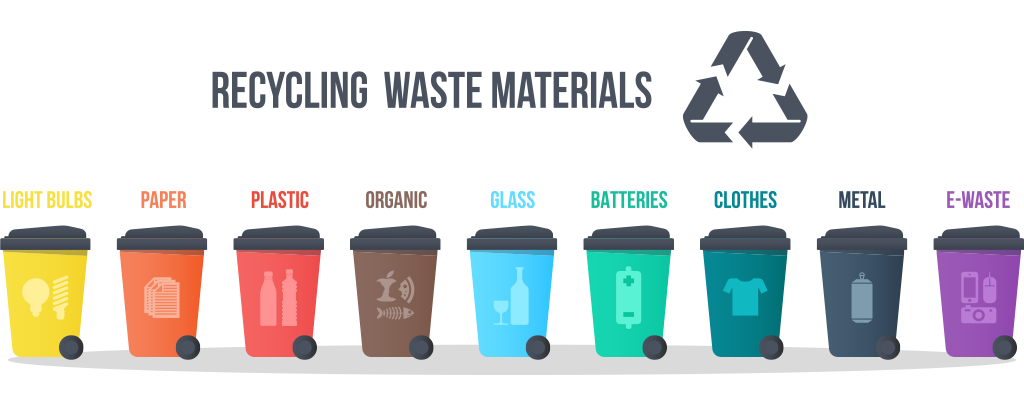
\includegraphics[width=5.20833in,height=\textheight]{assets/images/waste.png}
\end{center}

\section[{1. Are we aware?} ]{\texorpdfstring{{1. Are we aware?}
\protect
\includegraphics[width=1.13542in,height=0.28125in]{assets/images/trash.jpg}}{1. Are we aware? }}\label{are-we-aware}

\textbf{\emph{Important fact:}} Are we aware that when we do not recycle
waste or use it for energy consumption, it pollutes our groundwater, our
soil, and the air through greenhouse gases emitted by the waste,
ultimately reducing the quality of the food produced in our soil and our
overall life quality?

We just complain, don't we? Strawberries used to smell like
strawberries, tomatoes used to taste different\ldots{} right?

Unfortunately, complaining doesn't fix anything, and it won't. If we
want to deserve to live in this world, we must work hard for our
generation. The effort we do not put into our waste will heavily come
back to haunt us and our children in this universe created with karma.
\textbf{Let's quit complaining and start acting!}

\begin{center}
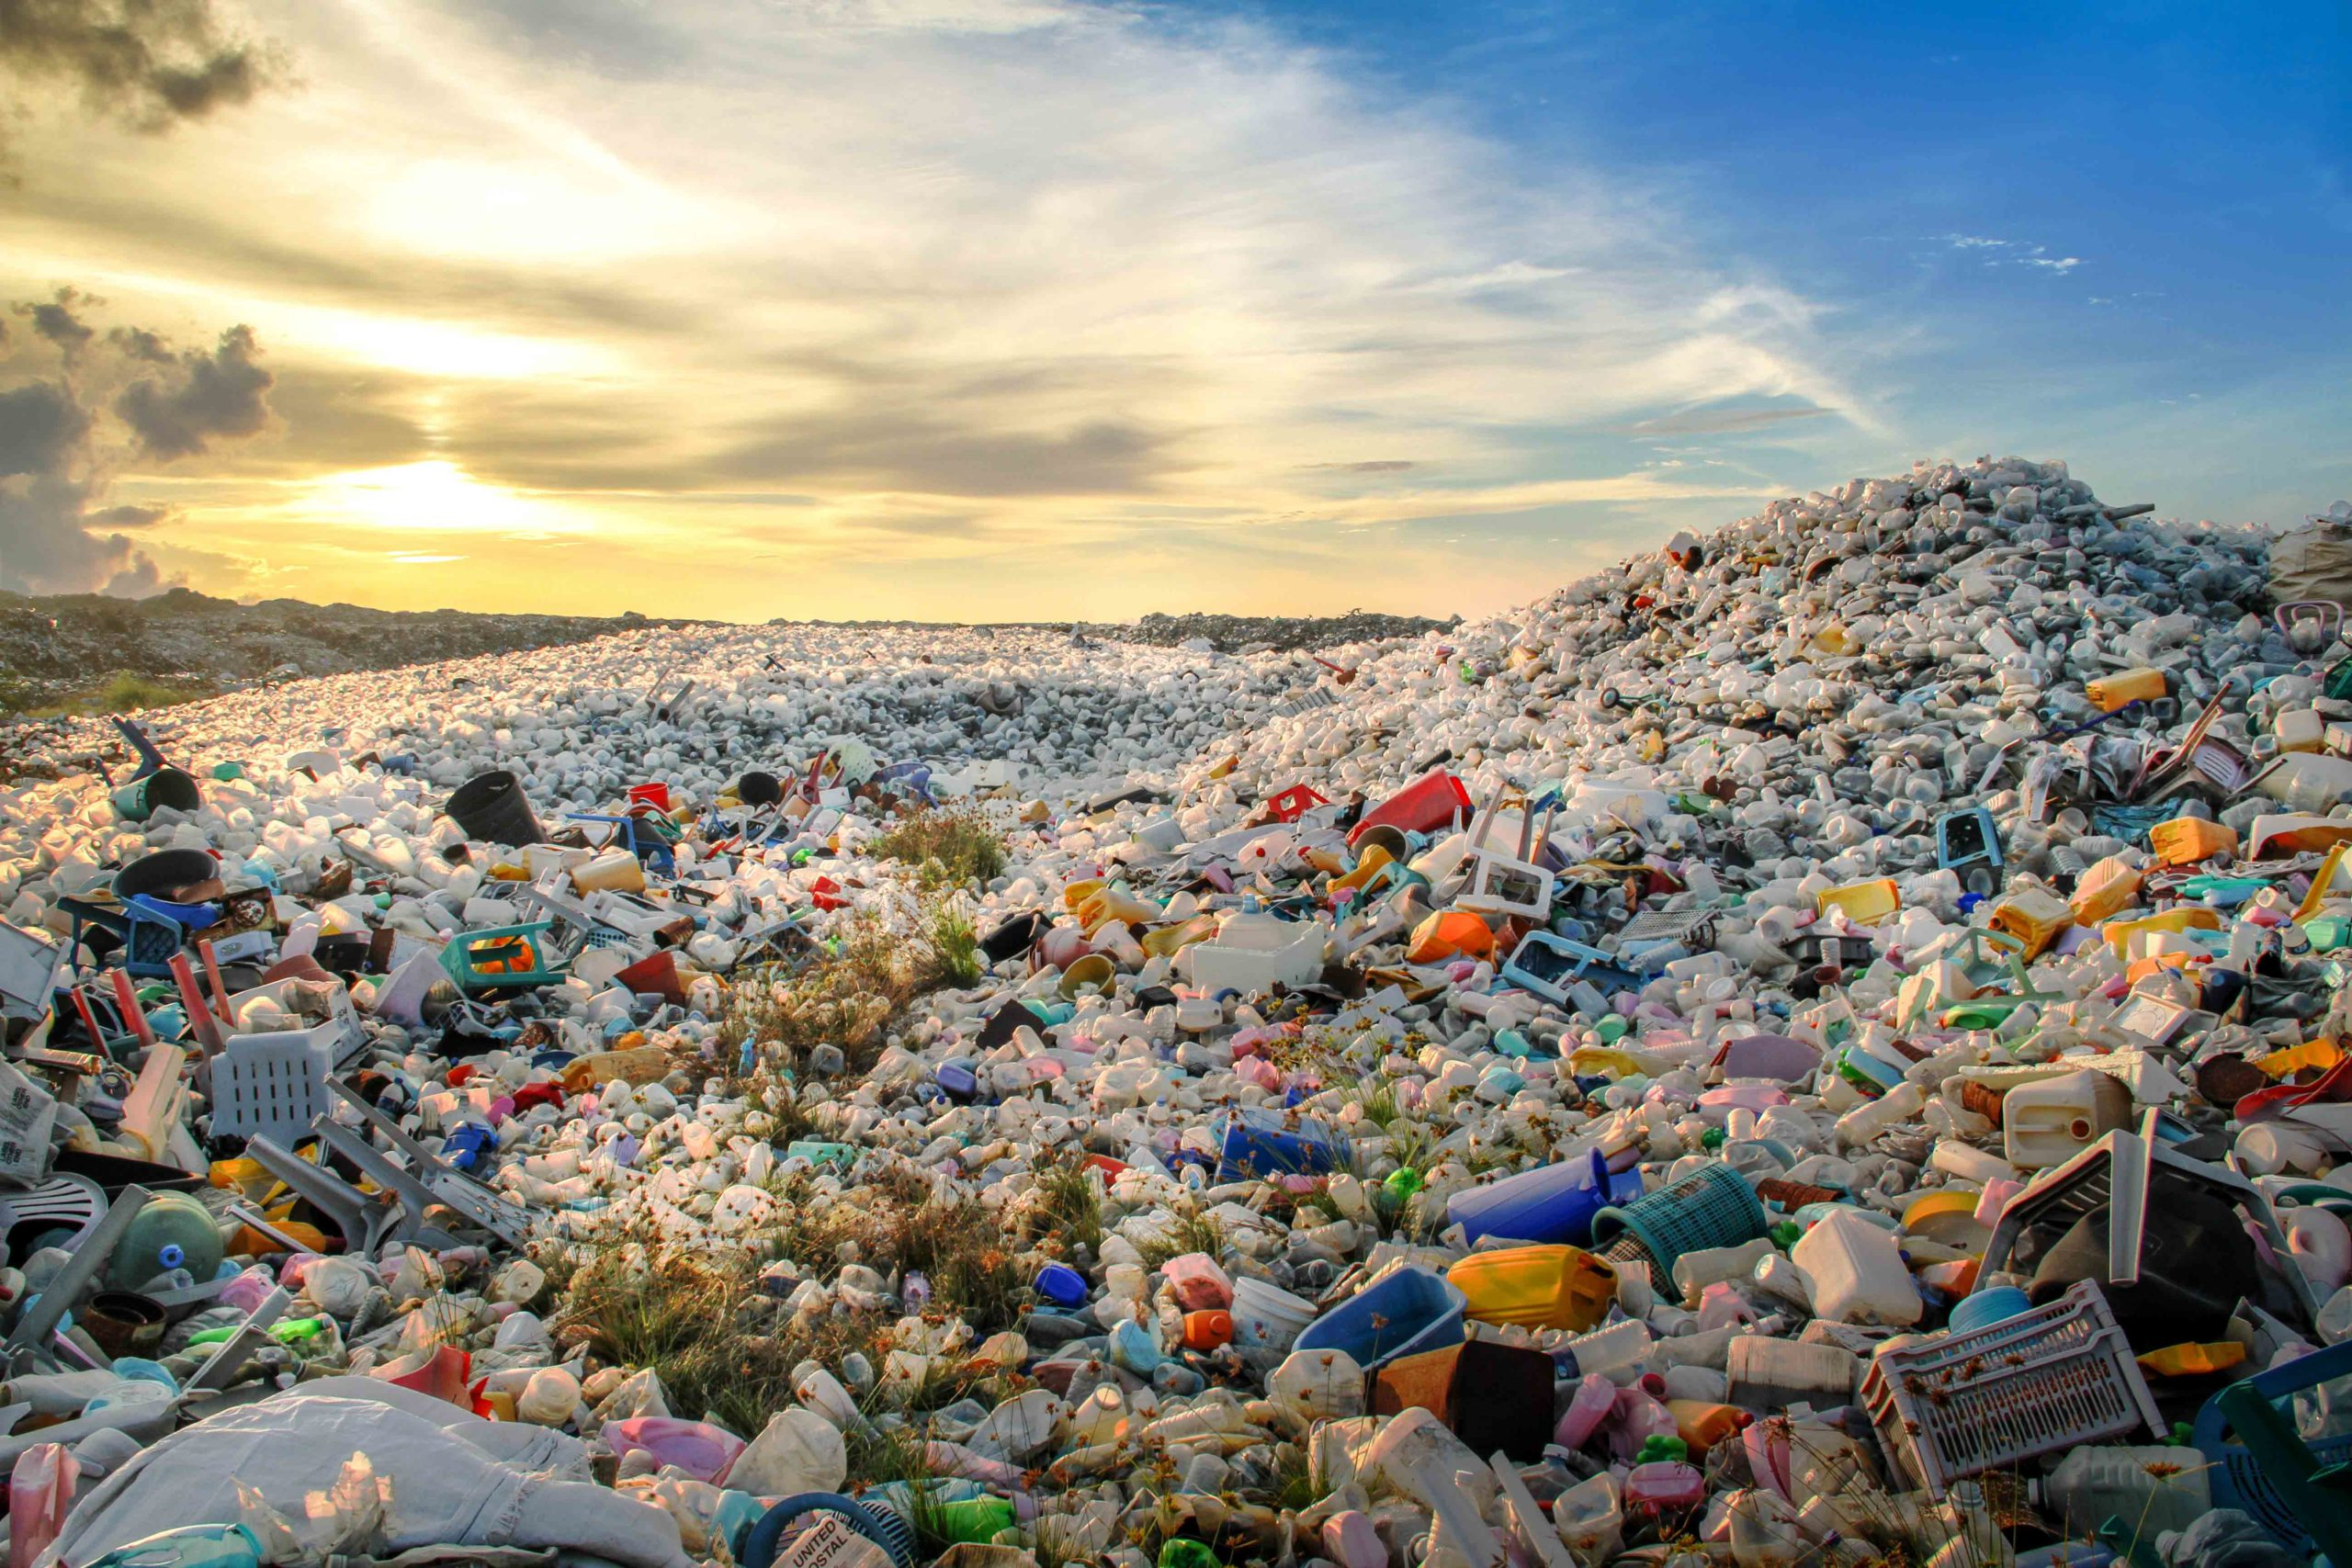
\includegraphics[width=3.125in,height=\textheight]{assets/images/landfill-scaled.jpg}
\end{center}

\textbf{\emph{The scope:}} The processes and activities required to
handle waste from its inception to its final disposal are called
\textbf{\emph{waste management.}} These activities include the
collection, transport, treatment, and disposal of waste, as well as the
monitoring and organization of waste management processes {[}1{]}. In
this project, insights are attempted to be extracted from several data
collections on waste management in Turkiye, with a particular focus on
municipal waste statistics. Initially, data are analyzed on a national
level, then the analysis is moved to a provincial basis. Then, time
series methods are used to forecast waste amount trends in Turkiye.
Additionally, the variables that influence the amounts of waste and
their effects by province are investigated using regression analysis.

\textbf{\emph{The aim:}} In this project, the main goals are to increase
awareness about waste issues, determine future waste quantities,
investigate the waste levels of the provinces, and discuss both
prevention strategies and proper disposal and recycling methods for
unavoidable waste.

\textbf{\emph{Some information before the analysis:}} As of 2023,
\textbf{\emph{Turkiye's population is 85 million 279 thousand 553
people}} and it has a total of 81 provinces, with Istanbul, Ankara, and
Izmir being the most populous {[}2{]}. According to the data from 2022,
\textbf{\emph{1,389}} out of 1,391 municipalities in Turkiye
\textbf{\emph{provide waste management services}}, and it is amassed
\textbf{\emph{a total of 30,283,757 tons of waste}}, and the amount of
MSW collected per person is \textbf{\emph{1.03 kg/day}} {[}3{]}. From
this total, \textbf{\emph{85.9\%}} was directed towards waste treatment
facilities, \textbf{\emph{13.5\%}} was allocated to municipal dumping
sites, and the remaining \textbf{\emph{0.6\%}} was disposed of through
alternative methods such as open burning, burial, and the dumping into
rivers or onto land {[}3{]}.

\section[{2. Data} ]{\texorpdfstring{{2. Data}
\protect
\includegraphics[width=0.44792in,height=0.30208in]{assets/images/data_symbol.jpg}}{2. Data }}\label{data}

{\textbf{\emph{Municipal Solid Waste (MSW)}}}, waste collected by the
municipalities that provide waste management services, includes everyday
trash from homes, businesses, and public places, along with bulky items
and yard waste. It also covers street sweepings and waste from public
trash bins and markets, if treated like household trash. However, it
doesn't include waste from sewer systems, industrial processes or
construction and demolition sites {[}4{]}.

Multiple data sources are planned to be utilized for the analysis in
this area of MSW, primarily focusing on waste quantities, along with
Gross Domestic Product (GDP), education, electricity consumption,
population figures, and agriculture area for \textbf{\emph{Turkiye and
its provinces.}}

\subsection[{2.1 Data Source} ]{\texorpdfstring{{2.1 Data Source}
\protect
\includegraphics[width=0.73958in,height=0.30208in]{assets/images/database.jpg}}{2.1 Data Source }}\label{data-source}

The references from which I have gathered the data include:

\begin{itemize}
\tightlist
\item
  \href{https://data.tuik.gov.tr/Bulten/Index?p=Waste-Statistics-2022-49570}{Waste
  Statistics, TURKSTAT}
\item
  \href{https://biruni.tuik.gov.tr/bolgeselistatistik/}{Environment
  Regional Data, Biruni TURKSTAT}
\item
  \href{https://biruni.tuik.gov.tr/bolgeselistatistik/}{Agriculture
  area, Biruni TURKSTAT}
\item
  \href{https://biruni.tuik.gov.tr/bolgeselistatistik/}{Education,
  Biruni TURKSTAT}
\item
  \href{https://biruni.tuik.gov.tr/bolgeselistatistik/}{GDP, Biruni
  TURKSTAT}
\item
  \href{https://biruni.tuik.gov.tr/bolgeselistatistik/}{Electricity
  consumption, Biruni TURKSTAT}
\end{itemize}

\subsection[{2.2 General Information About the Main Data}
]{\texorpdfstring{{2.2 General Information About the Main Data}
\protect
\includegraphics[width=0.27083in,height=0.23958in]{assets/images/info.jpg}}{2.2 General Information About the Main Data }}\label{general-information-about-the-main-data}

\begin{itemize}
\tightlist
\item
  \textbf{First data set:} The municipal waste amount data of Turkiye,
  which includes information such as the population of Turkiye and its
  81 provinces' municipalities, total waste amounts for the year 2022,
  the average waste amount per person, etc.
\end{itemize}

\begin{Shaded}
\begin{Highlighting}[]
\FunctionTok{library}\NormalTok{(openxlsx)}
\end{Highlighting}
\end{Shaded}

\begin{verbatim}
Warning: package 'openxlsx' was built under R version 4.3.3
\end{verbatim}

\begin{Shaded}
\begin{Highlighting}[]
\NormalTok{municipal\_waste }\OtherTok{\textless{}{-}} \FunctionTok{read.xlsx}\NormalTok{(}\StringTok{"project/data/municipal\_waste.xlsx"}\NormalTok{)}
\end{Highlighting}
\end{Shaded}

\begin{itemize}
\tightlist
\item
  \textbf{Second data set:} Data including the amounts of collected
  municipal waste that are sent to municipal landfills, waste processing
  facilities (the waste sent to landfill sites, incineration plants and
  all the waste recovery facilities), and disposed of using other
  methods (disposals by burning in an open area, dumping into river/onto
  land and burying).
\end{itemize}

\begin{Shaded}
\begin{Highlighting}[]
\NormalTok{where\_to\_municipal\_waste }\OtherTok{\textless{}{-}} \FunctionTok{read.xlsx}\NormalTok{(}\StringTok{"project/data/where\_to\_municipal\_waste.xlsx"}\NormalTok{)}
\end{Highlighting}
\end{Shaded}

\begin{itemize}
\tightlist
\item
  \textbf{Third data set:} Time series data including municipal waste
  amounts, waste per capita, waste sent to processing facilities, etc.,
  and time series of waste amounts by provinces of Turkiye for the years
  1994-2022.
\end{itemize}

\begin{Shaded}
\begin{Highlighting}[]
\NormalTok{time\_series\_municipal\_waste }\OtherTok{\textless{}{-}} \FunctionTok{read.xlsx}\NormalTok{(}\StringTok{"project/data/time\_series\_municipal\_waste.xlsx"}\NormalTok{, }\AttributeTok{colNames =} \ConstantTok{TRUE}\NormalTok{)}
\NormalTok{ts\_province }\OtherTok{\textless{}{-}} \FunctionTok{read.xlsx}\NormalTok{(}\StringTok{"project/data/ts\_waste\_province.xlsx"}\NormalTok{)}
\end{Highlighting}
\end{Shaded}

\subsection[{2.3 Reason of Choice} ]{\texorpdfstring{{2.3 Reason of
Choice}
\protect
\includegraphics[width=0.26042in,height=0.21875in]{assets/images/reason.jpg}}{2.3 Reason of Choice }}\label{reason-of-choice}

This topic was chosen because it was realized that \textbf{waste
management is not given enough importance} in Turkiye, and it is
believed that carelessness should not continue in this matter. The
importance of the subject is \textbf{indisputable}. By using the data
sets mentioned above, it is aimed to reveal and analyze the current
situation of waste management, to derive knowledge, and to contribute to
the literature and our country.

\subsection[{2.4 Preprocessing} ]{\texorpdfstring{{2.4 Preprocessing}
\protect
\includegraphics[width=0.30208in,height=0.25in]{assets/images/preprocess.jpg}}{2.4 Preprocessing }}\label{preprocessing}

\begin{itemize}
\tightlist
\item
  \textbf{For ``municipal\_waste'' dataset:}
\end{itemize}

\href{https://github.com/emu-hacettepe-analytics/emu660-spring2024-Dilara-pro/tree/main/project/data}{Downloadable
dataset in .RData version}

\begin{Shaded}
\begin{Highlighting}[]
\FunctionTok{library}\NormalTok{(tidyverse)}
\end{Highlighting}
\end{Shaded}

\begin{verbatim}
Warning: package 'stringr' was built under R version 4.3.2
\end{verbatim}

\begin{verbatim}
-- Attaching core tidyverse packages ------------------------ tidyverse 2.0.0 --
v dplyr     1.1.3     v readr     2.1.4
v forcats   1.0.0     v stringr   1.5.1
v ggplot2   3.4.4     v tibble    3.2.1
v lubridate 1.9.3     v tidyr     1.3.0
v purrr     1.0.2     
-- Conflicts ------------------------------------------ tidyverse_conflicts() --
x dplyr::filter() masks stats::filter()
x dplyr::lag()    masks stats::lag()
i Use the conflicted package (<http://conflicted.r-lib.org/>) to force all conflicts to become errors
\end{verbatim}

\begin{Shaded}
\begin{Highlighting}[]
\CommentTok{\# remove unnecessary columns}
\NormalTok{municipal\_waste }\OtherTok{\textless{}{-}} \FunctionTok{select}\NormalTok{(municipal\_waste, }\SpecialCharTok{{-}}\NormalTok{X5)    }
\NormalTok{municipal\_waste }\OtherTok{\textless{}{-}} \FunctionTok{select}\NormalTok{(municipal\_waste, }\SpecialCharTok{{-}}\NormalTok{X6)}
\CommentTok{\# rename columns}
\NormalTok{municipal\_waste }\OtherTok{\textless{}{-}} \FunctionTok{rename}\NormalTok{(municipal\_waste, }\StringTok{"Provinces"} \OtherTok{=}\StringTok{"Belediye.atık.hizmeti.istatistikleri,.2022.Municipal.waste.services.statistics,.2022"}\NormalTok{)}
\NormalTok{municipal\_waste }\OtherTok{\textless{}{-}} \FunctionTok{rename}\NormalTok{(municipal\_waste, }\StringTok{"Total municipal population"} \OtherTok{=} \StringTok{"X2"}\NormalTok{)}
\NormalTok{municipal\_waste }\OtherTok{\textless{}{-}} \FunctionTok{rename}\NormalTok{(municipal\_waste, }\StringTok{"Total number of municipalities"} \OtherTok{=}\StringTok{"X3"}\NormalTok{)}
\NormalTok{municipal\_waste }\OtherTok{\textless{}{-}} \FunctionTok{rename}\NormalTok{(municipal\_waste, }\StringTok{"Number of municipalities providing waste services"} \OtherTok{=}\StringTok{"X4"}\NormalTok{)}
\NormalTok{municipal\_waste }\OtherTok{\textless{}{-}} \FunctionTok{rename}\NormalTok{(municipal\_waste, }\StringTok{"Amount of waste collected (Tonnes) }
\StringTok{"} \OtherTok{=}\StringTok{"X7"}\NormalTok{)}
\NormalTok{municipal\_waste }\OtherTok{\textless{}{-}} \FunctionTok{rename}\NormalTok{(municipal\_waste, }\StringTok{"Amount of waste per capita (Kg/capita{-}day) }
\StringTok{"} \OtherTok{=}\StringTok{"X8"}\NormalTok{)}
\CommentTok{\# remove unnecessary rows}
\NormalTok{municipal\_waste }\OtherTok{\textless{}{-}}\NormalTok{ municipal\_waste[}\SpecialCharTok{{-}}\FunctionTok{c}\NormalTok{(}\DecValTok{1}\NormalTok{, }\DecValTok{2}\NormalTok{, }\DecValTok{85}\NormalTok{, }\DecValTok{86}\NormalTok{, }\DecValTok{87}\NormalTok{, }\DecValTok{88}\NormalTok{), ]}
\CommentTok{\# reorder row names that is disordered}
\FunctionTok{row.names}\NormalTok{(municipal\_waste) }\OtherTok{\textless{}{-}} \ConstantTok{NULL}
\NormalTok{municipal\_waste }\OtherTok{\textless{}{-}}\NormalTok{ municipal\_waste }\SpecialCharTok{\%\textgreater{}\%}
  \FunctionTok{mutate}\NormalTok{(}\AttributeTok{row\_id =} \FunctionTok{row\_number}\NormalTok{())  }
\NormalTok{municipal\_waste }\OtherTok{\textless{}{-}}\NormalTok{ municipal\_waste }\SpecialCharTok{\%\textgreater{}\%}
  \FunctionTok{select}\NormalTok{(row\_id, }\FunctionTok{everything}\NormalTok{()) }
\NormalTok{municipal\_waste }\OtherTok{\textless{}{-}}\NormalTok{ municipal\_waste[,}\SpecialCharTok{{-}}\FunctionTok{c}\NormalTok{(}\DecValTok{1}\NormalTok{)]}
\CommentTok{\# adjust necessary columns as numbers}
\NormalTok{municipal\_waste }\OtherTok{\textless{}{-}}\NormalTok{ municipal\_waste }\SpecialCharTok{\%\textgreater{}\%}
  \FunctionTok{mutate}\NormalTok{(}\FunctionTok{across}\NormalTok{(}\SpecialCharTok{{-}}\NormalTok{Provinces, }\SpecialCharTok{\textasciitilde{}}\FunctionTok{as.numeric}\NormalTok{(}\FunctionTok{as.character}\NormalTok{(.))))}
\FunctionTok{sapply}\NormalTok{(municipal\_waste,class)}
\end{Highlighting}
\end{Shaded}

\begin{verbatim}
                                        Provinces 
                                      "character" 
                       Total municipal population 
                                        "numeric" 
                   Total number of municipalities 
                                        "numeric" 
Number of municipalities providing waste services 
                                        "numeric" 
            Amount of waste collected (Tonnes) \n 
                                        "numeric" 
    Amount of waste per capita (Kg/capita-day) \n 
                                        "numeric" 
\end{verbatim}

The first six rows of the municipal waste dataset are provided below.

\begin{Shaded}
\begin{Highlighting}[]
\FunctionTok{str}\NormalTok{(municipal\_waste)}
\end{Highlighting}
\end{Shaded}

\begin{verbatim}
'data.frame':   82 obs. of  6 variables:
 $ Provinces                                        : chr  "Türkiye" "Adana" "Adıyaman" "Afyonkarahisar" ...
 $ Total municipal population                       : num  80785141 2274106 487642 588048 314539 ...
 $ Total number of municipalities                   : num  1391 16 23 60 12 ...
 $ Number of municipalities providing waste services: num  1389 16 22 60 12 ...
 $ Amount of waste collected (Tonnes) 
            : num  30283757 665695 179724 198273 181116 ...
 $ Amount of waste per capita (Kg/capita-day) 
    : num  1.033 0.807 1.019 0.928 1.58 ...
\end{verbatim}

The descriptive statistics for each column are provided below.

\begin{Shaded}
\begin{Highlighting}[]
\FunctionTok{summary}\NormalTok{(municipal\_waste)}
\end{Highlighting}
\end{Shaded}

\begin{verbatim}
  Provinces         Total municipal population Total number of municipalities
 Length:82          Min.   :   41120           Min.   :   4.00               
 Class :character   1st Qu.:  242100           1st Qu.:  11.00               
 Mode  :character   Median :  417945           Median :  16.00               
                    Mean   : 1970369           Mean   :  33.93               
                    3rd Qu.: 1139026           3rd Qu.:  21.00               
                    Max.   :80785141           Max.   :1391.00               
 Number of municipalities providing waste services
 Min.   :   4.00                                  
 1st Qu.:  11.00                                  
 Median :  16.00                                  
 Mean   :  33.88                                  
 3rd Qu.:  21.00                                  
 Max.   :1389.00                                  
 Amount of waste collected (Tonnes) \n
 Min.   :   21392                     
 1st Qu.:   81725                     
 Median :  151235                     
 Mean   :  738628                     
 3rd Qu.:  415882                     
 Max.   :30283757                     
 Amount of waste per capita (Kg/capita-day) \n
 Min.   :0.6498                               
 1st Qu.:0.8730                               
 Median :0.9672                               
 Mean   :1.0679                               
 3rd Qu.:1.1887                               
 Max.   :1.9962                               
\end{verbatim}

\begin{itemize}
\tightlist
\item
  \textbf{For ``where\_to\_municipal\_waste'' dataset:}
\end{itemize}

\href{https://github.com/emu-hacettepe-analytics/emu660-spring2024-Dilara-pro/tree/main/project/data}{Downloadable
dataset in .RData version}

\begin{Shaded}
\begin{Highlighting}[]
\FunctionTok{library}\NormalTok{(tidyverse)}
\CommentTok{\# remove unnecessary columns}
\NormalTok{where\_to\_municipal\_waste }\OtherTok{\textless{}{-}} \FunctionTok{select}\NormalTok{(where\_to\_municipal\_waste, }\SpecialCharTok{{-}}\NormalTok{X2)    }
\NormalTok{where\_to\_municipal\_waste }\OtherTok{\textless{}{-}} \FunctionTok{select}\NormalTok{(where\_to\_municipal\_waste, }\SpecialCharTok{{-}}\NormalTok{X4)}
\NormalTok{where\_to\_municipal\_waste }\OtherTok{\textless{}{-}} \FunctionTok{select}\NormalTok{(where\_to\_municipal\_waste, }\SpecialCharTok{{-}}\NormalTok{X6)}
\NormalTok{where\_to\_municipal\_waste }\OtherTok{\textless{}{-}} \FunctionTok{select}\NormalTok{(where\_to\_municipal\_waste, }\SpecialCharTok{{-}}\NormalTok{X8)}
\NormalTok{where\_to\_municipal\_waste }\OtherTok{\textless{}{-}} \FunctionTok{select}\NormalTok{(where\_to\_municipal\_waste, }\SpecialCharTok{{-}}\NormalTok{X9)}
\CommentTok{\# rename columns}
\NormalTok{where\_to\_municipal\_waste }\OtherTok{\textless{}{-}} \FunctionTok{rename}\NormalTok{(where\_to\_municipal\_waste, }\StringTok{"Provinces"} \OtherTok{=} \StringTok{\textasciigrave{}}\AttributeTok{Belediye.atık.yönetimi.istatistikleri,.2022.Municipal.waste.management.statistics,.2022}\StringTok{\textasciigrave{}}\NormalTok{)}
\NormalTok{where\_to\_municipal\_waste }\OtherTok{\textless{}{-}} \FunctionTok{rename}\NormalTok{(where\_to\_municipal\_waste, }\StringTok{"Total amount of waste collected  (Tonnes)"} \OtherTok{=} \StringTok{"X3"}\NormalTok{)}
\NormalTok{where\_to\_municipal\_waste }\OtherTok{\textless{}{-}} \FunctionTok{rename}\NormalTok{(where\_to\_municipal\_waste, }\StringTok{"Municipality\textquotesingle{}s dumping sites"} \OtherTok{=}\StringTok{"X5"}\NormalTok{)}
\NormalTok{where\_to\_municipal\_waste }\OtherTok{\textless{}{-}} \FunctionTok{rename}\NormalTok{(where\_to\_municipal\_waste, }\StringTok{"Waste treatment facilities"}\OtherTok{=} \StringTok{"X7"}\NormalTok{)}
\NormalTok{where\_to\_municipal\_waste }\OtherTok{\textless{}{-}} \FunctionTok{rename}\NormalTok{(where\_to\_municipal\_waste, }\StringTok{"Other disposal methods"}\OtherTok{=} \StringTok{"X10"}\NormalTok{)}
\CommentTok{\# remove unnecessary rows}
\NormalTok{where\_to\_municipal\_waste }\OtherTok{\textless{}{-}}\NormalTok{ where\_to\_municipal\_waste[}\SpecialCharTok{{-}}\FunctionTok{c}\NormalTok{(}\DecValTok{1}\NormalTok{, }\DecValTok{2}\NormalTok{, }\DecValTok{85}\SpecialCharTok{:}\DecValTok{94}\NormalTok{), ]}
\CommentTok{\# reorder row names that is disordered}
\FunctionTok{row.names}\NormalTok{(where\_to\_municipal\_waste) }\OtherTok{\textless{}{-}} \ConstantTok{NULL}
\NormalTok{where\_to\_municipal\_waste }\OtherTok{\textless{}{-}}\NormalTok{ where\_to\_municipal\_waste }\SpecialCharTok{\%\textgreater{}\%}
  \FunctionTok{mutate}\NormalTok{(}\AttributeTok{row\_id =} \FunctionTok{row\_number}\NormalTok{())  }
\NormalTok{where\_to\_municipal\_waste }\OtherTok{\textless{}{-}}\NormalTok{ where\_to\_municipal\_waste }\SpecialCharTok{\%\textgreater{}\%}
  \FunctionTok{select}\NormalTok{(row\_id, }\FunctionTok{everything}\NormalTok{()) }
\NormalTok{where\_to\_municipal\_waste }\OtherTok{\textless{}{-}}\NormalTok{ where\_to\_municipal\_waste[,}\SpecialCharTok{{-}}\FunctionTok{c}\NormalTok{(}\DecValTok{1}\NormalTok{)]}
\CommentTok{\# adjust necessary columns as numbers}
\NormalTok{where\_to\_municipal\_waste }\OtherTok{\textless{}{-}}\NormalTok{ where\_to\_municipal\_waste }\SpecialCharTok{\%\textgreater{}\%}
  \FunctionTok{mutate}\NormalTok{(}\FunctionTok{across}\NormalTok{(}\SpecialCharTok{{-}}\NormalTok{Provinces, }\SpecialCharTok{\textasciitilde{}}\FunctionTok{as.numeric}\NormalTok{(}\FunctionTok{as.character}\NormalTok{(.))))}
\FunctionTok{sapply}\NormalTok{(where\_to\_municipal\_waste,class)}
\end{Highlighting}
\end{Shaded}

\begin{verbatim}
                                Provinces 
                              "character" 
Total amount of waste collected  (Tonnes) 
                                "numeric" 
             Municipality's dumping sites 
                                "numeric" 
               Waste treatment facilities 
                                "numeric" 
                   Other disposal methods 
                                "numeric" 
\end{verbatim}

The first six rows of the dataset showing the distribution of municipal
waste disposal methods are provided below.

\begin{Shaded}
\begin{Highlighting}[]
\FunctionTok{str}\NormalTok{(where\_to\_municipal\_waste)}
\end{Highlighting}
\end{Shaded}

\begin{verbatim}
'data.frame':   82 obs. of  5 variables:
 $ Provinces                                : chr  "Türkiye" "Adana" "Adıyaman" "Afyonkarahisar" ...
 $ Total amount of waste collected  (Tonnes): num  30283757 665695 179724 198273 181116 ...
 $ Municipality's dumping sites             : num  4092721 0 178453 20090 131116 ...
 $ Waste treatment facilities               : num  26016988 663895 1271 175952 50000 ...
 $ Other disposal methods                   : num  174048 1800 0 2231 0 ...
\end{verbatim}

The descriptive statistics for each column are provided below.

\begin{Shaded}
\begin{Highlighting}[]
\FunctionTok{summary}\NormalTok{(where\_to\_municipal\_waste)}
\end{Highlighting}
\end{Shaded}

\begin{verbatim}
  Provinces         Total amount of waste collected  (Tonnes)
 Length:82          Min.   :   21392                         
 Class :character   1st Qu.:   81725                         
 Mode  :character   Median :  151235                         
                    Mean   :  738628                         
                    3rd Qu.:  415882                         
                    Max.   :30283757                         
 Municipality's dumping sites Waste treatment facilities Other disposal methods
 Min.   :      0              Min.   :       0           Min.   :     0.0      
 1st Qu.:   1260              1st Qu.:   52770           1st Qu.:     0.0      
 Median :  17376              Median :  109595           Median :     0.0      
 Mean   :  99822              Mean   :  634561           Mean   :  4245.1      
 3rd Qu.:  56501              3rd Qu.:  333389           3rd Qu.:   557.5      
 Max.   :4092721              Max.   :26016988           Max.   :174047.6      
\end{verbatim}

\begin{itemize}
\tightlist
\item
  \textbf{For ``time\_series\_municipal\_waste'' dataset and
  ``ts\_province'' dataset:}
\end{itemize}

\href{https://github.com/emu-hacettepe-analytics/emu660-spring2024-Dilara-pro/tree/main/project/data}{Downloadable
dataset in .RData version}

\begin{Shaded}
\begin{Highlighting}[]
\FunctionTok{library}\NormalTok{(tidyverse)}
\CommentTok{\# remove unnecessary rows}
\NormalTok{time\_series\_municipal\_waste }\OtherTok{\textless{}{-}}\NormalTok{ time\_series\_municipal\_waste[}\SpecialCharTok{{-}}\FunctionTok{c}\NormalTok{(}\DecValTok{2}\SpecialCharTok{:}\DecValTok{6}\NormalTok{,}\DecValTok{10}\NormalTok{,}\DecValTok{14}\SpecialCharTok{:}\DecValTok{43}\NormalTok{), ]}
\NormalTok{time\_series\_municipal\_waste }\OtherTok{\textless{}{-}} \FunctionTok{rename}\NormalTok{(time\_series\_municipal\_waste, }\StringTok{"Waste/Year"} \OtherTok{=} \StringTok{"X1"}\NormalTok{)}
\CommentTok{\# rename rows}
\NormalTok{time\_series\_municipal\_waste[}\DecValTok{1}\NormalTok{,}\DecValTok{1}\NormalTok{] }\OtherTok{\textless{}{-}} \StringTok{"Turkey population"}
\NormalTok{time\_series\_municipal\_waste[}\DecValTok{2}\NormalTok{,}\DecValTok{1}\NormalTok{] }\OtherTok{\textless{}{-}} \StringTok{"Amount of municipal waste generated (Thousand tonnes/year)"}
\NormalTok{time\_series\_municipal\_waste[}\DecValTok{3}\NormalTok{,}\DecValTok{1}\NormalTok{] }\OtherTok{\textless{}{-}} \StringTok{"Amount of municipal waste collected (Thousand tonnes/year)"}
\NormalTok{time\_series\_municipal\_waste[}\DecValTok{4}\NormalTok{,}\DecValTok{1}\NormalTok{] }\OtherTok{\textless{}{-}} \StringTok{"Average amount of municipal waste per capita (Kg/capita{-}day)"}
\NormalTok{time\_series\_municipal\_waste[}\DecValTok{5}\NormalTok{,}\DecValTok{1}\NormalTok{] }\OtherTok{\textless{}{-}} \StringTok{"Waste treatment facilities"}
\NormalTok{time\_series\_municipal\_waste[}\DecValTok{6}\NormalTok{,}\DecValTok{1}\NormalTok{] }\OtherTok{\textless{}{-}} \StringTok{"Municipality\textquotesingle{}s dumping sites"}
\NormalTok{time\_series\_municipal\_waste[}\DecValTok{7}\NormalTok{,}\DecValTok{1}\NormalTok{] }\OtherTok{\textless{}{-}} \StringTok{"Other disposal methods"}
\CommentTok{\# reorder row names that is disordered}
\FunctionTok{row.names}\NormalTok{(time\_series\_municipal\_waste) }\OtherTok{\textless{}{-}} \ConstantTok{NULL}
\CommentTok{\# adjust necessary columns as numbers}
\NormalTok{time\_series\_municipal\_waste }\OtherTok{\textless{}{-}}\NormalTok{ time\_series\_municipal\_waste }\SpecialCharTok{\%\textgreater{}\%}
  \FunctionTok{mutate}\NormalTok{(}\FunctionTok{across}\NormalTok{(}\SpecialCharTok{{-}}\StringTok{\textasciigrave{}}\AttributeTok{Waste/Year}\StringTok{\textasciigrave{}}\NormalTok{, }\SpecialCharTok{\textasciitilde{}}\FunctionTok{as.numeric}\NormalTok{(}\FunctionTok{as.character}\NormalTok{(.))))}
\FunctionTok{sapply}\NormalTok{(time\_series\_municipal\_waste,class)}
\end{Highlighting}
\end{Shaded}

\begin{verbatim}
 Waste/Year        1994        1995        1996        1997        1998 
"character"   "numeric"   "numeric"   "numeric"   "numeric"   "numeric" 
       2001        2002        2003        2004        2006        2008 
  "numeric"   "numeric"   "numeric"   "numeric"   "numeric"   "numeric" 
       2010        2012        2014        2016        2018        2020 
  "numeric"   "numeric"   "numeric"   "numeric"   "numeric"   "numeric" 
       2022 
  "numeric" 
\end{verbatim}

The attributes of the time series dataset are provided below.

\begin{Shaded}
\begin{Highlighting}[]
\FunctionTok{str}\NormalTok{(time\_series\_municipal\_waste)}
\end{Highlighting}
\end{Shaded}

\begin{verbatim}
'data.frame':   7 obs. of  19 variables:
 $ Waste/Year: chr  "Turkey population" "Amount of municipal waste generated (Thousand tonnes/year)" "Amount of municipal waste collected (Thousand tonnes/year)" "Average amount of municipal waste per capita (Kg/capita-day)" ...
 $ 1994      : num  6.28e+07 2.34e+04 1.78e+04 1.10 1.00e+03 ...
 $ 1995      : num  6.28e+07 2.72e+04 2.09e+04 1.27 1.60e+03 ...
 $ 1996      : num  6.28e+07 2.93e+04 2.25e+04 1.37 3.03e+03 ...
 $ 1997      : num  6.28e+07 3.19e+04 2.42e+04 1.46 4.54e+03 ...
 $ 1998      : num  6.28e+07 3.30e+04 2.49e+04 1.51 5.42e+03 ...
 $ 2001      : num  6.78e+07 3.10e+04 2.51e+04 1.35 8.52e+03 ...
 $ 2002      : num  6.78e+07 3.10e+04 2.54e+04 1.34 7.43e+03 ...
 $ 2003      : num  6.78e+07 3.11e+04 2.61e+04 1.38 7.76e+03 ...
 $ 2004      : num  6.78e+07 2.97e+04 2.50e+04 1.31 7.35e+03 ...
 $ 2006      : num  7.06e+07 3.01e+04 2.53e+04 1.21 9.68e+03 ...
 $ 2008      : num  7.06e+07 2.85e+04 2.44e+04 1.15 1.12e+04 ...
 $ 2010      : num  7.37e+07 2.97e+04 2.53e+04 1.14 1.39e+04 ...
 $ 2012      : num  7.56e+07 3.08e+04 2.58e+04 1.12 1.56e+04 ...
 $ 2014      : num  7.77e+07 3.12e+04 2.80e+04 1.08 1.79e+04 ...
 $ 2016      : num  7.98e+07 3.38e+04 3.16e+04 1.17 2.24e+04 ...
 $ 2018      : num  8.20e+07 3.45e+04 3.22e+04 1.16 2.56e+04 ...
 $ 2020      : num  8.36e+07 3.48e+04 3.23e+04 1.13 2.67e+04 ...
 $ 2022      : num  8.53e+07 3.24e+04 3.03e+04 1.03 2.60e+04 ...
\end{verbatim}

The attributes of the provinces' time series dataset are provided below.

\begin{Shaded}
\begin{Highlighting}[]
\NormalTok{ts\_province  }\OtherTok{\textless{}{-}} \FunctionTok{select}\NormalTok{(ts\_province , }\SpecialCharTok{{-}}\NormalTok{BÖLGE.KODU)  }
\NormalTok{ts\_province  }\OtherTok{\textless{}{-}} \FunctionTok{rename}\NormalTok{(ts\_province , }\StringTok{"Year"} \OtherTok{=}\NormalTok{ YIL)}
\NormalTok{ts\_province  }\OtherTok{\textless{}{-}} \FunctionTok{rename}\NormalTok{(ts\_province , }\StringTok{"Province"} \OtherTok{=}\NormalTok{ BÖLGE.ADI)}
\NormalTok{ts\_province  }\OtherTok{\textless{}{-}} \FunctionTok{rename}\NormalTok{(ts\_province , }\StringTok{"Waste amount (1000 ton)"} \OtherTok{=} \StringTok{\textasciigrave{}}\AttributeTok{Belediye.atık.istatistikleri.:.Toplanan.atık.miktarı.(1000.ton)}\StringTok{\textasciigrave{}}\NormalTok{)}
\NormalTok{ts\_province}\SpecialCharTok{$}\NormalTok{Year }\OtherTok{\textless{}{-}} \FunctionTok{as.numeric}\NormalTok{(ts\_province}\SpecialCharTok{$}\NormalTok{Year)}
\NormalTok{ts\_province}\SpecialCharTok{$}\StringTok{\textasciigrave{}}\AttributeTok{Waste amount (1000 ton)}\StringTok{\textasciigrave{}} \OtherTok{\textless{}{-}} \FunctionTok{as.numeric}\NormalTok{(ts\_province}\SpecialCharTok{$}\StringTok{\textasciigrave{}}\AttributeTok{Waste amount (1000 ton)}\StringTok{\textasciigrave{}}\NormalTok{)}
\end{Highlighting}
\end{Shaded}

\begin{verbatim}
Warning: Zorlamadan dolayı ortaya çıkan NAs
\end{verbatim}

\begin{Shaded}
\begin{Highlighting}[]
\FunctionTok{str}\NormalTok{(ts\_province)}
\end{Highlighting}
\end{Shaded}

\begin{verbatim}
'data.frame':   1134 obs. of  3 variables:
 $ Year                   : num  1998 2001 2002 2003 2004 ...
 $ Province               : chr  "İstanbul" "İstanbul" "İstanbul" "İstanbul" ...
 $ Waste amount (1000 ton): num  6074 6112 5231 5375 4471 ...
\end{verbatim}

\section[{3. Analysis} ]{\texorpdfstring{{3. Analysis}
\protect
\includegraphics[width=0.375in,height=0.30208in]{assets/images/analysis.jpg}}{3. Analysis }}\label{analysis}

In the first phase of this section, \emph{Exploratory Data Analysis
(EDA)}, the data prepared for analysis is visualized to enable
discoveries that are not immediately apparent at first glance. Later,
relationships are determined through \emph{regression analysis}, future
predictions are made using \emph{time series methods}.

\subsection[{3.1 Exploratory Data Analysis} ]{\texorpdfstring{{3.1
Exploratory Data Analysis}
\protect
\includegraphics[width=0.23958in,height=0.21875in]{assets/images/EDA.jpg}}{3.1 Exploratory Data Analysis }}\label{exploratory-data-analysis}

{\textbf{For ``municipal\_waste'' dataset:}}

The relationship between the population size of Turkiye provinces and
the amount of waste generated is shown in the scatter plot below.
According to the plot, a linear relationship is observed between them.

\begin{Shaded}
\begin{Highlighting}[]
\FunctionTok{library}\NormalTok{(tidyverse)}
\FunctionTok{library}\NormalTok{(ggthemes)}
\end{Highlighting}
\end{Shaded}

\begin{verbatim}
Warning: package 'ggthemes' was built under R version 4.3.2
\end{verbatim}

\begin{Shaded}
\begin{Highlighting}[]
\FunctionTok{library}\NormalTok{(ggrepel)}
\end{Highlighting}
\end{Shaded}

\begin{verbatim}
Warning: package 'ggrepel' was built under R version 4.3.2
\end{verbatim}

\begin{Shaded}
\begin{Highlighting}[]
\NormalTok{municipal\_waste }\OtherTok{\textless{}{-}}\NormalTok{ municipal\_waste[}\SpecialCharTok{{-}}\FunctionTok{c}\NormalTok{(}\DecValTok{1}\NormalTok{), ]}

\NormalTok{p }\OtherTok{\textless{}{-}}\NormalTok{ municipal\_waste }\SpecialCharTok{|\textgreater{}} \FunctionTok{ggplot}\NormalTok{(}\FunctionTok{aes}\NormalTok{(}\StringTok{\textasciigrave{}}\AttributeTok{Total municipal population}\StringTok{\textasciigrave{}}\SpecialCharTok{/}\DecValTok{10}\SpecialCharTok{\^{}}\DecValTok{6}\NormalTok{, }
\StringTok{\textasciigrave{}}\AttributeTok{Amount of waste collected (Tonnes) }
\StringTok{\textasciigrave{}}\SpecialCharTok{/}\DecValTok{10}\SpecialCharTok{\^{}}\DecValTok{4}\NormalTok{)) }
\NormalTok{p }\SpecialCharTok{+} \FunctionTok{geom\_point}\NormalTok{(}\AttributeTok{color =} \StringTok{"skyblue"}\NormalTok{) }\SpecialCharTok{+} 
\FunctionTok{scale\_x\_continuous}\NormalTok{(}\AttributeTok{trans =} \StringTok{"log10"}\NormalTok{) }\SpecialCharTok{+}
\FunctionTok{scale\_y\_continuous}\NormalTok{(}\AttributeTok{trans =} \StringTok{"log10"}\NormalTok{) }\SpecialCharTok{+}
\FunctionTok{xlab}\NormalTok{(}\StringTok{"Total municipal population (million)"}\NormalTok{) }\SpecialCharTok{+}
\FunctionTok{ylab}\NormalTok{(}\StringTok{"Amount of waste collected (kg)"}\NormalTok{) }\SpecialCharTok{+}
\FunctionTok{ggtitle}\NormalTok{(}\StringTok{"Amount of waste in Turkiye\textquotesingle{}s provinces"}\NormalTok{)}\SpecialCharTok{+} 
\FunctionTok{theme\_classic}\NormalTok{()}
\end{Highlighting}
\end{Shaded}

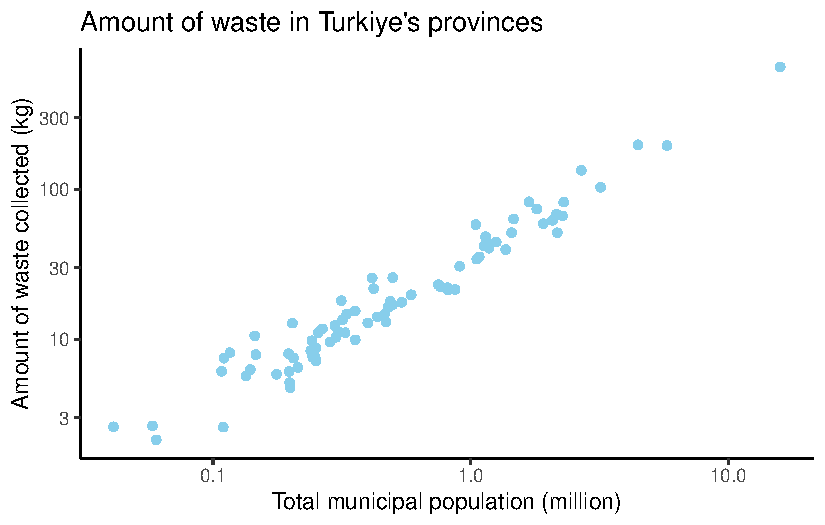
\includegraphics{project_files/figure-pdf/unnamed-chunk-13-1.pdf}

Provinces ranked according to the total number of municipalities can be
seen in the below graph together with the number of municipalities.

\begin{Shaded}
\begin{Highlighting}[]
\NormalTok{p }\OtherTok{\textless{}{-}} \FunctionTok{ggplot}\NormalTok{(municipal\_waste, }\FunctionTok{aes}\NormalTok{(}\AttributeTok{x =} \FunctionTok{reorder}\NormalTok{(Provinces, }\StringTok{\textasciigrave{}}\AttributeTok{Total number of municipalities}\StringTok{\textasciigrave{}}\NormalTok{, }\AttributeTok{FUN =}\NormalTok{ sum), }\AttributeTok{y =} \StringTok{\textasciigrave{}}\AttributeTok{Total number of municipalities}\StringTok{\textasciigrave{}}\NormalTok{)) }
\NormalTok{p }\SpecialCharTok{+} \FunctionTok{geom\_bar}\NormalTok{(}\AttributeTok{stat =} \StringTok{"identity"}\NormalTok{, }\AttributeTok{fill=} \StringTok{"purple"}\NormalTok{) }\SpecialCharTok{+} 
  \FunctionTok{xlab}\NormalTok{(}\StringTok{"Provinces"}\NormalTok{) }\SpecialCharTok{+}
  \FunctionTok{theme\_calc}\NormalTok{() }\SpecialCharTok{+}
  \FunctionTok{ggtitle}\NormalTok{(}\StringTok{"Number of municipalities in provinces"}\NormalTok{) }\SpecialCharTok{+} 
  \FunctionTok{theme}\NormalTok{(}\AttributeTok{axis.text.x =} \FunctionTok{element\_text}\NormalTok{(}\AttributeTok{angle =} \DecValTok{90}\NormalTok{, }\AttributeTok{hjust =} \DecValTok{1}\NormalTok{, }\AttributeTok{size =} \DecValTok{6}\NormalTok{)) }
\end{Highlighting}
\end{Shaded}

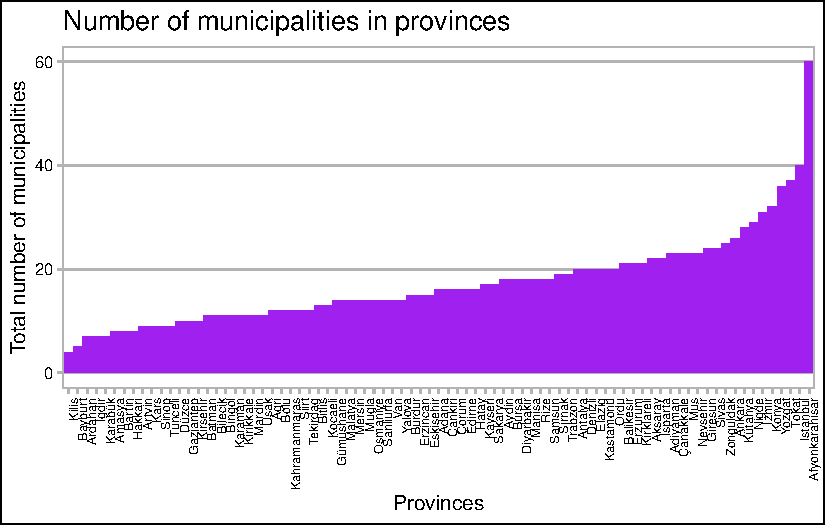
\includegraphics{project_files/figure-pdf/unnamed-chunk-14-1.pdf}

In the plot below, the first 20 provinces with the highest amount of
waste per capita and their populations can be found.

\begin{Shaded}
\begin{Highlighting}[]
\CommentTok{\# The provinces that produce largest amount of waste}
\NormalTok{The\_largest }\OtherTok{\textless{}{-}}\NormalTok{ municipal\_waste }\SpecialCharTok{|\textgreater{}} \FunctionTok{arrange}\NormalTok{(}\FunctionTok{desc}\NormalTok{(}\StringTok{\textasciigrave{}}\AttributeTok{Amount of waste per capita (Kg/capita{-}day) }
\StringTok{\textasciigrave{}}\NormalTok{)) }\SpecialCharTok{|\textgreater{}} \FunctionTok{head}\NormalTok{(}\AttributeTok{n =} \DecValTok{20}\NormalTok{)}
\NormalTok{p }\OtherTok{\textless{}{-}} \FunctionTok{ggplot}\NormalTok{(The\_largest, }\FunctionTok{aes}\NormalTok{(}\AttributeTok{x =} \FunctionTok{reorder}\NormalTok{(Provinces, }\StringTok{\textasciigrave{}}\AttributeTok{Amount of waste per capita (Kg/capita{-}day) }
\StringTok{\textasciigrave{}}\NormalTok{, }\AttributeTok{FUN =}\NormalTok{ sum),}
                             \AttributeTok{y =} \StringTok{\textasciigrave{}}\AttributeTok{Amount of waste per capita (Kg/capita{-}day) }
\StringTok{\textasciigrave{}}\NormalTok{))}
\FunctionTok{ggplot}\NormalTok{(The\_largest, }\FunctionTok{aes}\NormalTok{(}\AttributeTok{x =}\StringTok{\textasciigrave{}}\AttributeTok{Amount of waste per capita (Kg/capita{-}day) }
\StringTok{\textasciigrave{}}\NormalTok{, }\AttributeTok{y =} \FunctionTok{reorder}\NormalTok{(Provinces, }\StringTok{\textasciigrave{}}\AttributeTok{Amount of waste per capita (Kg/capita{-}day) }
\StringTok{\textasciigrave{}}\NormalTok{, }\AttributeTok{FUN =}\NormalTok{ sum), }\AttributeTok{color =} \StringTok{\textasciigrave{}}\AttributeTok{Amount of waste per capita (Kg/capita{-}day) }
\StringTok{\textasciigrave{}}\NormalTok{)) }\SpecialCharTok{+}
  \FunctionTok{geom\_point}\NormalTok{(}\AttributeTok{size =} \DecValTok{4}\NormalTok{) }\SpecialCharTok{+}
  \FunctionTok{geom\_segment}\NormalTok{(}\FunctionTok{aes}\NormalTok{(}\AttributeTok{xend =} \DecValTok{1}\NormalTok{, }\AttributeTok{yend =}\NormalTok{ Provinces), }\AttributeTok{linewidth =} \DecValTok{1}\NormalTok{) }\SpecialCharTok{+} 
  \FunctionTok{ylab}\NormalTok{(}\StringTok{"Provinces"}\NormalTok{) }\SpecialCharTok{+}
  \FunctionTok{ggtitle}\NormalTok{(}\StringTok{"Provinces with the largest waste amount"}\NormalTok{)}\SpecialCharTok{+}
  \FunctionTok{geom\_text\_repel}\NormalTok{(}\FunctionTok{aes}\NormalTok{(}\AttributeTok{label =}\StringTok{\textasciigrave{}}\AttributeTok{Total municipal population}\StringTok{\textasciigrave{}}\NormalTok{), }\AttributeTok{color =} \StringTok{"black"}\NormalTok{, }\AttributeTok{size =} \DecValTok{2}\NormalTok{)}
\end{Highlighting}
\end{Shaded}

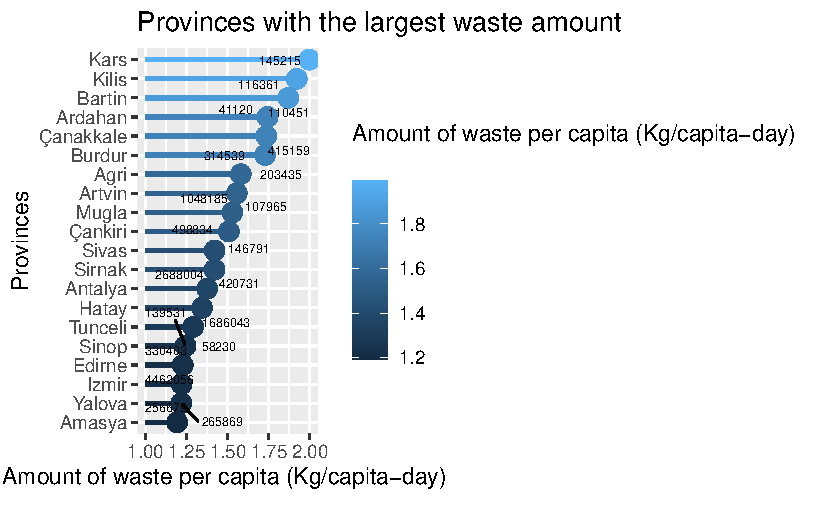
\includegraphics{project_files/figure-pdf/unnamed-chunk-15-1.pdf}

{\textbf{For ``where\_to\_municipal\_waste'' dataset:}}

The distribution of waste collected by municipalities according to three
disposal methods and provinces is analysed in this section.

\begin{Shaded}
\begin{Highlighting}[]
\FunctionTok{library}\NormalTok{(tidyverse)}
\FunctionTok{library}\NormalTok{(ggthemes)}
\FunctionTok{library}\NormalTok{(ggrepel)}
\FunctionTok{library}\NormalTok{(dplyr)}

\NormalTok{dumping\_site }\OtherTok{\textless{}{-}}\NormalTok{where\_to\_municipal\_waste }\SpecialCharTok{|\textgreater{}} 
  \FunctionTok{mutate}\NormalTok{(}\AttributeTok{proportion1 =} \StringTok{\textasciigrave{}}\AttributeTok{Municipality\textquotesingle{}s dumping sites}\StringTok{\textasciigrave{}}\SpecialCharTok{/}\StringTok{\textasciigrave{}}\AttributeTok{Total amount of waste collected  (Tonnes)}\StringTok{\textasciigrave{}}\NormalTok{)}
\NormalTok{treatment\_facility }\OtherTok{\textless{}{-}}\NormalTok{where\_to\_municipal\_waste }\SpecialCharTok{|\textgreater{}} 
  \FunctionTok{mutate}\NormalTok{(}\AttributeTok{proportion2 =}\StringTok{\textasciigrave{}}\AttributeTok{Waste treatment facilities}\StringTok{\textasciigrave{}}\SpecialCharTok{/}\StringTok{\textasciigrave{}}\AttributeTok{Total amount of waste collected  (Tonnes)}\StringTok{\textasciigrave{}}\NormalTok{)}
\NormalTok{other\_disposal }\OtherTok{\textless{}{-}}\NormalTok{where\_to\_municipal\_waste }\SpecialCharTok{|\textgreater{}} 
  \FunctionTok{mutate}\NormalTok{(}\AttributeTok{proportion3 =}\StringTok{\textasciigrave{}}\AttributeTok{Other disposal methods}\StringTok{\textasciigrave{}}\SpecialCharTok{/}\StringTok{\textasciigrave{}}\AttributeTok{Total amount of waste collected  (Tonnes)}\StringTok{\textasciigrave{}}\NormalTok{)}
\end{Highlighting}
\end{Shaded}

The amount of waste allocated for the \emph{municipality dumping site}
can be seen below, plotted by province, with circle diameters
representing the total amount of waste.

\begin{Shaded}
\begin{Highlighting}[]
\CommentTok{\# Dumping site proportion graph}
\NormalTok{dumping\_site }\OtherTok{\textless{}{-}}\NormalTok{ dumping\_site[}\SpecialCharTok{{-}}\FunctionTok{c}\NormalTok{(}\DecValTok{1}\NormalTok{), ]}
\FunctionTok{ggplot}\NormalTok{(dumping\_site, }\FunctionTok{aes}\NormalTok{(Provinces, proportion1, }\AttributeTok{size =}\StringTok{\textasciigrave{}}\AttributeTok{Total amount of waste collected  (Tonnes)}\StringTok{\textasciigrave{}}\SpecialCharTok{/} \DecValTok{10}\SpecialCharTok{\^{}}\DecValTok{4}\NormalTok{)) }\SpecialCharTok{+}
  \FunctionTok{geom\_point}\NormalTok{(}\AttributeTok{color =} \StringTok{"blue"}\NormalTok{, }\AttributeTok{alpha =} \FloatTok{0.6}\NormalTok{) }\SpecialCharTok{+} \FunctionTok{theme}\NormalTok{(}\AttributeTok{axis.text.x =} \FunctionTok{element\_text}\NormalTok{(}\AttributeTok{angle =} \DecValTok{90}\NormalTok{, }\AttributeTok{hjust =} \DecValTok{1}\NormalTok{, }\AttributeTok{size =} \DecValTok{6}\NormalTok{)) }\SpecialCharTok{+}
  \FunctionTok{labs}\NormalTok{ (}\AttributeTok{x =} \StringTok{"Provinces"}\NormalTok{,}\AttributeTok{y =} \StringTok{"Proportion for dumping site"}\NormalTok{, }\AttributeTok{title =} \StringTok{"Proportion of wastes sent"}\NormalTok{, }\AttributeTok{size =} \StringTok{"Total waste (kg)"}\NormalTok{) }\SpecialCharTok{+}  \FunctionTok{coord\_cartesian}\NormalTok{(}\AttributeTok{ylim =} \FunctionTok{c}\NormalTok{(}\DecValTok{0}\NormalTok{, }\DecValTok{1}\NormalTok{))}
\end{Highlighting}
\end{Shaded}

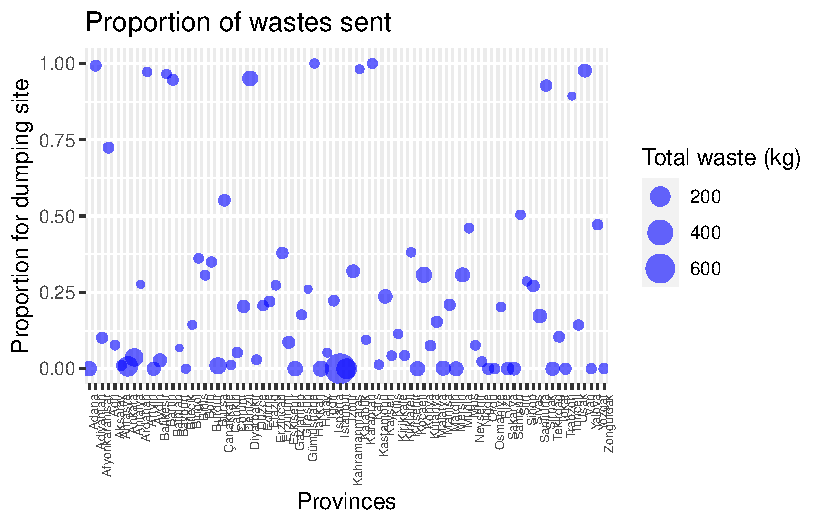
\includegraphics{project_files/figure-pdf/unnamed-chunk-17-1.pdf}

The amount of waste allocated for the \emph{waste treatment facilities}
can be seen below, plotted by province, with circle diameters
representing the total amount of waste.

\begin{Shaded}
\begin{Highlighting}[]
\CommentTok{\# Waste treatment facility proportion graph}
\NormalTok{treatment\_facility }\OtherTok{\textless{}{-}}\NormalTok{ treatment\_facility[}\SpecialCharTok{{-}}\FunctionTok{c}\NormalTok{(}\DecValTok{1}\NormalTok{), ]}
\FunctionTok{ggplot}\NormalTok{(treatment\_facility, }\FunctionTok{aes}\NormalTok{(Provinces, proportion2, }\AttributeTok{size =}\StringTok{\textasciigrave{}}\AttributeTok{Total amount of waste collected  (Tonnes)}\StringTok{\textasciigrave{}}\SpecialCharTok{/} \DecValTok{10}\SpecialCharTok{\^{}}\DecValTok{4}\NormalTok{)) }\SpecialCharTok{+}
  \FunctionTok{geom\_point}\NormalTok{(}\AttributeTok{color =} \StringTok{"orange"}\NormalTok{, }\AttributeTok{alpha =} \FloatTok{0.6}\NormalTok{) }\SpecialCharTok{+}  \FunctionTok{theme}\NormalTok{(}\AttributeTok{axis.text.x =} \FunctionTok{element\_text}\NormalTok{(}\AttributeTok{angle =} \DecValTok{90}\NormalTok{, }\AttributeTok{hjust =} \DecValTok{1}\NormalTok{, }\AttributeTok{size =} \DecValTok{6}\NormalTok{)) }\SpecialCharTok{+}
  \FunctionTok{labs}\NormalTok{ (}\AttributeTok{x =} \StringTok{"Provinces"}\NormalTok{,}\AttributeTok{y =} \StringTok{"Proportion for waste treatment facility"}\NormalTok{, }\AttributeTok{title =} \StringTok{"Proportion of wastes sent"}\NormalTok{, }\AttributeTok{size =} \StringTok{"Total waste (kg)"}\NormalTok{) }\SpecialCharTok{+} \FunctionTok{coord\_cartesian}\NormalTok{(}\AttributeTok{ylim =} \FunctionTok{c}\NormalTok{(}\DecValTok{0}\NormalTok{, }\DecValTok{1}\NormalTok{)) }
\end{Highlighting}
\end{Shaded}

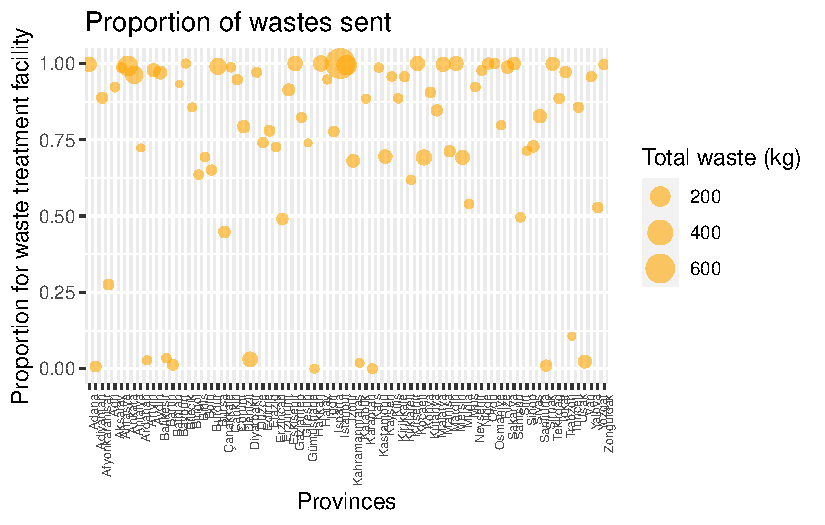
\includegraphics{project_files/figure-pdf/unnamed-chunk-18-1.pdf}

The amount of waste allocated for the \emph{other disposal methods} can
be seen below, plotted by province, with circle diameters representing
the total amount of waste.

\begin{Shaded}
\begin{Highlighting}[]
\CommentTok{\# Other disposal methods proportion graph}
\NormalTok{other\_disposal }\OtherTok{\textless{}{-}}\NormalTok{ other\_disposal[}\SpecialCharTok{{-}}\FunctionTok{c}\NormalTok{(}\DecValTok{1}\NormalTok{), ]}
\FunctionTok{ggplot}\NormalTok{(other\_disposal, }\FunctionTok{aes}\NormalTok{(Provinces, proportion3, }\AttributeTok{size =}\StringTok{\textasciigrave{}}\AttributeTok{Total amount of waste collected  (Tonnes)}\StringTok{\textasciigrave{}}\SpecialCharTok{/} \DecValTok{10}\SpecialCharTok{\^{}}\DecValTok{4}\NormalTok{)) }\SpecialCharTok{+}
  \FunctionTok{geom\_point}\NormalTok{(}\AttributeTok{color =} \StringTok{"darkgreen"}\NormalTok{, }\AttributeTok{alpha =} \FloatTok{0.6}\NormalTok{) }\SpecialCharTok{+} \FunctionTok{theme}\NormalTok{(}\AttributeTok{axis.text.x =} \FunctionTok{element\_text}\NormalTok{(}\AttributeTok{angle =} \DecValTok{90}\NormalTok{, }\AttributeTok{hjust =} \DecValTok{1}\NormalTok{, }\AttributeTok{size =} \DecValTok{6}\NormalTok{)) }\SpecialCharTok{+}
  \FunctionTok{labs}\NormalTok{ (}\AttributeTok{x =} \StringTok{"Provinces"}\NormalTok{,}\AttributeTok{y =} \StringTok{"Pro. for other disposal methods"}\NormalTok{, }\AttributeTok{title =} \StringTok{"Proportion of wastes sent"}\NormalTok{, }\AttributeTok{size =} \StringTok{"Total waste (kg)"}\NormalTok{) }\SpecialCharTok{+} \FunctionTok{coord\_cartesian}\NormalTok{(}\AttributeTok{ylim =} \FunctionTok{c}\NormalTok{(}\DecValTok{0}\NormalTok{, }\DecValTok{1}\NormalTok{))}
\end{Highlighting}
\end{Shaded}

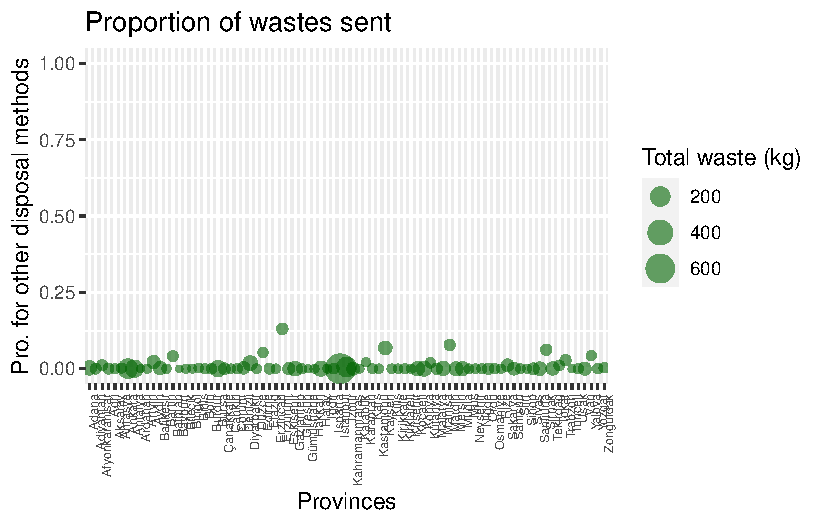
\includegraphics{project_files/figure-pdf/unnamed-chunk-19-1.pdf}

The pie chart below shows a rough breakdown of the amount of waste sent
to these three disposal methods.

\begin{Shaded}
\begin{Highlighting}[]
\CommentTok{\# Pie Chart}
\NormalTok{waste\_distr }\OtherTok{\textless{}{-}} \FunctionTok{data.frame}\NormalTok{(}\AttributeTok{Method =} \FunctionTok{c}\NormalTok{(}\StringTok{"Municipality\textquotesingle{}s Dumping Site"}\NormalTok{, }\StringTok{"Waste Treatment Facilities"}\NormalTok{, }\StringTok{"Other Disposal Methods"}\NormalTok{), }\AttributeTok{Amount =} \FunctionTok{c}\NormalTok{(where\_to\_municipal\_waste[}\DecValTok{1}\NormalTok{,}\DecValTok{3}\NormalTok{]}\SpecialCharTok{/}\NormalTok{where\_to\_municipal\_waste[}\DecValTok{1}\NormalTok{,}\DecValTok{2}\NormalTok{], where\_to\_municipal\_waste[}\DecValTok{1}\NormalTok{,}\DecValTok{4}\NormalTok{]}\SpecialCharTok{/}\NormalTok{where\_to\_municipal\_waste[}\DecValTok{1}\NormalTok{,}\DecValTok{2}\NormalTok{], where\_to\_municipal\_waste[}\DecValTok{1}\NormalTok{,}\DecValTok{5}\NormalTok{]}\SpecialCharTok{/}\NormalTok{where\_to\_municipal\_waste[}\DecValTok{1}\NormalTok{,}\DecValTok{2}\NormalTok{]))}
\FunctionTok{ggplot}\NormalTok{(waste\_distr, }\FunctionTok{aes}\NormalTok{(}\AttributeTok{x =} \StringTok{""}\NormalTok{, }\AttributeTok{y =}\NormalTok{ Amount, }\AttributeTok{fill =}\NormalTok{ Method)) }\SpecialCharTok{+} 
  \FunctionTok{geom\_bar}\NormalTok{(}\AttributeTok{width =} \DecValTok{1}\NormalTok{, }\AttributeTok{stat =} \StringTok{"identity"}\NormalTok{) }\SpecialCharTok{+} 
  \FunctionTok{coord\_polar}\NormalTok{(}\AttributeTok{theta =} \StringTok{"y"}\NormalTok{) }\SpecialCharTok{+} 
  \FunctionTok{theme\_void}\NormalTok{() }\SpecialCharTok{+}
  \FunctionTok{labs}\NormalTok{(}\AttributeTok{title =} \StringTok{"Waste Disposal Methods"}\NormalTok{, }\AttributeTok{fill =} \StringTok{"Disposal Method"}\NormalTok{)}
\end{Highlighting}
\end{Shaded}

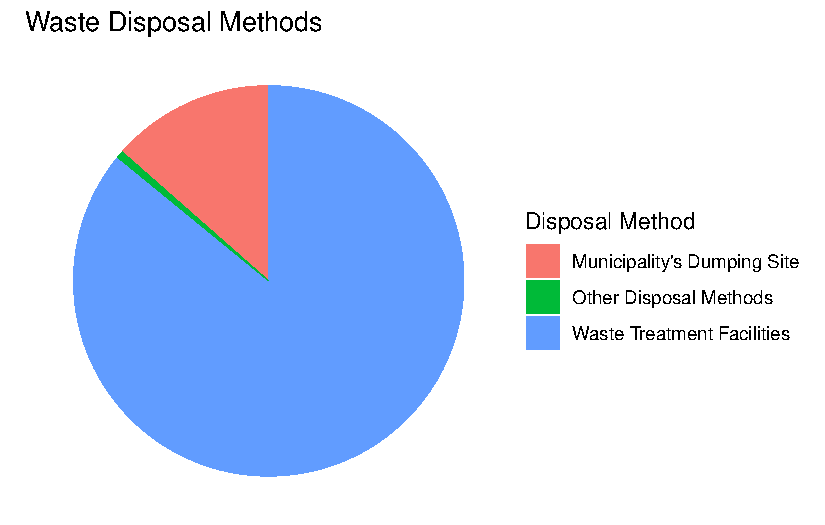
\includegraphics{project_files/figure-pdf/unnamed-chunk-20-1.pdf}

{\textbf{For ``time\_series\_municipal\_waste'' dataset and
``ts\_province'' dataset:}}

According to the time series data set, Turkiye's population change over
the years is given below.

\begin{Shaded}
\begin{Highlighting}[]
\FunctionTok{library}\NormalTok{(tidyverse)}
\FunctionTok{library}\NormalTok{(ggthemes)}
\FunctionTok{library}\NormalTok{(ggrepel)}
\FunctionTok{library}\NormalTok{(dplyr)}

\NormalTok{ts\_data }\OtherTok{\textless{}{-}}\NormalTok{ time\_series\_municipal\_waste }\SpecialCharTok{\%\textgreater{}\%}
  \FunctionTok{pivot\_longer}\NormalTok{(}\AttributeTok{cols =} \SpecialCharTok{{-}}\StringTok{\textasciigrave{}}\AttributeTok{Waste/Year}\StringTok{\textasciigrave{}}\NormalTok{, }\AttributeTok{names\_to =} \StringTok{"Year"}\NormalTok{, }\AttributeTok{values\_to =} \StringTok{"Value"}\NormalTok{) }\SpecialCharTok{\%\textgreater{}\%}
  \FunctionTok{mutate}\NormalTok{(}\AttributeTok{Year =} \FunctionTok{as.numeric}\NormalTok{(Year))  }

\CommentTok{\# Türkiye population ts}
\FunctionTok{ggplot}\NormalTok{(ts\_data }\SpecialCharTok{\%\textgreater{}\%} \FunctionTok{filter}\NormalTok{(}\StringTok{\textasciigrave{}}\AttributeTok{Waste/Year}\StringTok{\textasciigrave{}} \SpecialCharTok{==} \StringTok{"Turkey population"}\NormalTok{), }
                          \FunctionTok{aes}\NormalTok{(}\AttributeTok{x =}\NormalTok{ Year, }\AttributeTok{y =}\NormalTok{ Value }\SpecialCharTok{/} \DecValTok{10}\SpecialCharTok{\^{}}\DecValTok{6}\NormalTok{)) }\SpecialCharTok{+}
  \FunctionTok{geom\_line}\NormalTok{(}\AttributeTok{color =} \StringTok{"blue"}\NormalTok{) }\SpecialCharTok{+}
  \FunctionTok{geom\_point}\NormalTok{(}\AttributeTok{color =} \StringTok{"magenta"}\NormalTok{) }\SpecialCharTok{+}
  \FunctionTok{theme\_bw}\NormalTok{() }\SpecialCharTok{+} \FunctionTok{coord\_fixed}\NormalTok{() }\SpecialCharTok{+}
  \FunctionTok{labs}\NormalTok{(}\AttributeTok{title =} \StringTok{"Turkiye Population Over the Years"}\NormalTok{, }\AttributeTok{x =} \StringTok{"Year"}\NormalTok{, }\AttributeTok{y =} \StringTok{"Population (million)"}\NormalTok{)}
\end{Highlighting}
\end{Shaded}

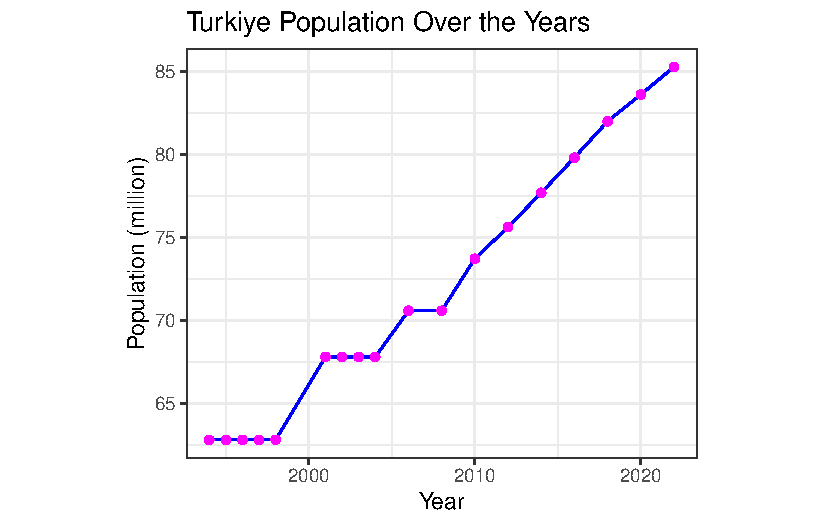
\includegraphics{project_files/figure-pdf/unnamed-chunk-21-1.pdf}

The relationship between the total amount of waste generated in Turkey
and the amount collected by municipalities for proper disposal can be
accessed from the plot.

\begin{Shaded}
\begin{Highlighting}[]
\CommentTok{\# Waste graphs}
\NormalTok{ts\_data2 }\OtherTok{\textless{}{-}}\NormalTok{ ts\_data }\SpecialCharTok{\%\textgreater{}\%}
  \FunctionTok{filter}\NormalTok{(}\StringTok{\textasciigrave{}}\AttributeTok{Waste/Year}\StringTok{\textasciigrave{}} \SpecialCharTok{\%in\%} \FunctionTok{c}\NormalTok{(}\StringTok{"Amount of municipal waste generated (Thousand tonnes/year)"}\NormalTok{, }
                             \StringTok{"Amount of municipal waste collected (Thousand tonnes/year)"}\NormalTok{)) }\SpecialCharTok{\%\textgreater{}\%}
  \FunctionTok{mutate}\NormalTok{(}\AttributeTok{Type =} \FunctionTok{case\_when}\NormalTok{(}
    \StringTok{\textasciigrave{}}\AttributeTok{Waste/Year}\StringTok{\textasciigrave{}} \SpecialCharTok{==} \StringTok{"Amount of municipal waste generated (Thousand tonnes/year)"} \SpecialCharTok{\textasciitilde{}} \StringTok{"Generated"}\NormalTok{,}
    \StringTok{\textasciigrave{}}\AttributeTok{Waste/Year}\StringTok{\textasciigrave{}} \SpecialCharTok{==} \StringTok{"Amount of municipal waste collected (Thousand tonnes/year)"} \SpecialCharTok{\textasciitilde{}} \StringTok{"Collected"}
\NormalTok{  ))}

\FunctionTok{ggplot}\NormalTok{(ts\_data2, }\FunctionTok{aes}\NormalTok{(}\AttributeTok{x =}\NormalTok{ Year, }\AttributeTok{y =}\NormalTok{ Value, }\AttributeTok{color =}\NormalTok{ Type, }\AttributeTok{group =}\NormalTok{ Type)) }\SpecialCharTok{+}
  \FunctionTok{geom\_line}\NormalTok{() }\SpecialCharTok{+}
  \FunctionTok{geom\_point}\NormalTok{() }\SpecialCharTok{+}
  \FunctionTok{scale\_color\_manual}\NormalTok{(}\AttributeTok{values =} \FunctionTok{c}\NormalTok{(}\StringTok{"Generated"} \OtherTok{=} \StringTok{"green"}\NormalTok{, }\StringTok{"Collected"} \OtherTok{=} \StringTok{"purple"}\NormalTok{)) }\SpecialCharTok{+}
  \FunctionTok{labs}\NormalTok{(}\AttributeTok{title =} \StringTok{"Municipal Waste Generated and Collected Over the Years"}\NormalTok{,}
       \AttributeTok{x =} \StringTok{"Year"}\NormalTok{, }
       \AttributeTok{y =} \StringTok{"Waste (Thousand tonnes)"}\NormalTok{,}
       \AttributeTok{color =} \StringTok{"Type"}\NormalTok{) }\SpecialCharTok{+} 
  \FunctionTok{theme\_minimal}\NormalTok{()}
\end{Highlighting}
\end{Shaded}

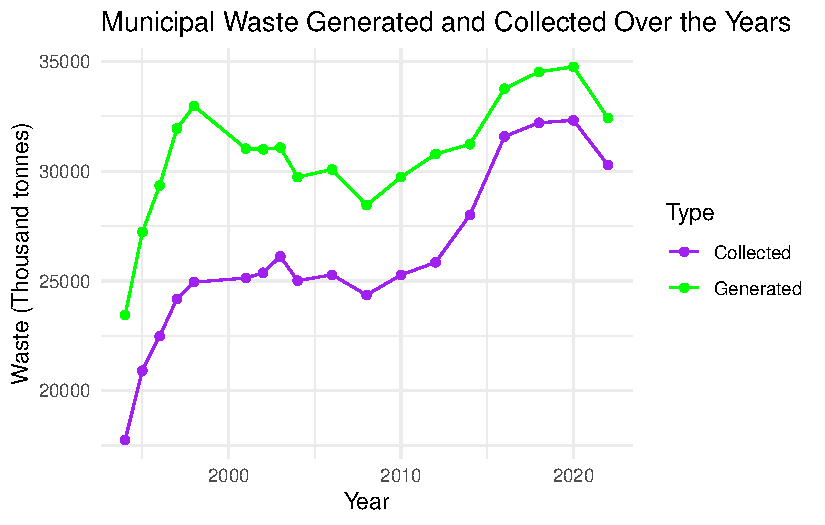
\includegraphics{project_files/figure-pdf/unnamed-chunk-22-1.pdf}

Changes in waste amount over the years according to disposal methods are
given below.

\begin{Shaded}
\begin{Highlighting}[]
\NormalTok{disposal\_methods\_data }\OtherTok{\textless{}{-}}\NormalTok{ ts\_data }\SpecialCharTok{\%\textgreater{}\%}
  \FunctionTok{filter}\NormalTok{(}\StringTok{\textasciigrave{}}\AttributeTok{Waste/Year}\StringTok{\textasciigrave{}} \SpecialCharTok{\%in\%} \FunctionTok{c}\NormalTok{(}\StringTok{"Waste treatment facilities"}\NormalTok{, }
                             \StringTok{"Municipality\textquotesingle{}s dumping sites"}\NormalTok{, }
                             \StringTok{"Other disposal methods"}\NormalTok{)) }\SpecialCharTok{\%\textgreater{}\%}
  \FunctionTok{mutate}\NormalTok{(}\AttributeTok{Type =} \FunctionTok{case\_when}\NormalTok{(}
    \StringTok{\textasciigrave{}}\AttributeTok{Waste/Year}\StringTok{\textasciigrave{}} \SpecialCharTok{==} \StringTok{"Waste treatment facilities"} \SpecialCharTok{\textasciitilde{}} \StringTok{"Waste Treatment"}\NormalTok{,}
    \StringTok{\textasciigrave{}}\AttributeTok{Waste/Year}\StringTok{\textasciigrave{}} \SpecialCharTok{==} \StringTok{"Municipality\textquotesingle{}s dumping sites"} \SpecialCharTok{\textasciitilde{}} \StringTok{"Dumping Sites"}\NormalTok{,}
    \StringTok{\textasciigrave{}}\AttributeTok{Waste/Year}\StringTok{\textasciigrave{}} \SpecialCharTok{==} \StringTok{"Other disposal methods"} \SpecialCharTok{\textasciitilde{}} \StringTok{"Other Methods"}
\NormalTok{  ))}

\FunctionTok{ggplot}\NormalTok{(disposal\_methods\_data, }\FunctionTok{aes}\NormalTok{(}\AttributeTok{x =}\NormalTok{ Year, }\AttributeTok{y =}\NormalTok{ Value, }\AttributeTok{color =}\NormalTok{ Type, }\AttributeTok{group =}\NormalTok{ Type)) }\SpecialCharTok{+}
  \FunctionTok{geom\_line}\NormalTok{() }\SpecialCharTok{+}
  \FunctionTok{geom\_point}\NormalTok{() }\SpecialCharTok{+}
  \FunctionTok{scale\_color\_manual}\NormalTok{(}\AttributeTok{values =} \FunctionTok{c}\NormalTok{(}\StringTok{"Waste Treatment"} \OtherTok{=} \StringTok{"blue"}\NormalTok{, }\StringTok{"Dumping Sites"} \OtherTok{=} \StringTok{"red"}\NormalTok{, }\StringTok{"Other Methods"} \OtherTok{=} \StringTok{"green"}\NormalTok{)) }\SpecialCharTok{+}
  \FunctionTok{labs}\NormalTok{(}\AttributeTok{title =} \StringTok{"Disposal Methods Over the Years"}\NormalTok{,}
       \AttributeTok{x =} \StringTok{"Year"}\NormalTok{, }
       \AttributeTok{y =} \StringTok{"Amount (Thousand tonnes)"}\NormalTok{,}
       \AttributeTok{color =} \StringTok{"Method"}\NormalTok{) }\SpecialCharTok{+}
  \FunctionTok{theme\_classic}\NormalTok{()}
\end{Highlighting}
\end{Shaded}

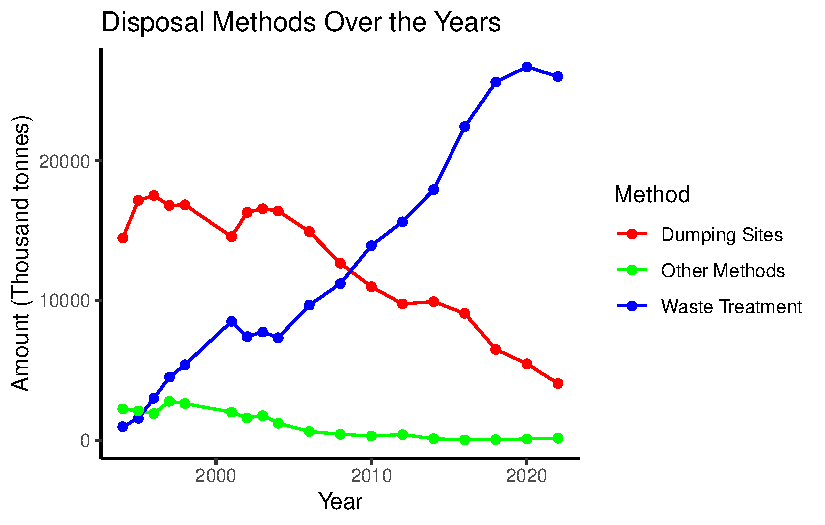
\includegraphics{project_files/figure-pdf/unnamed-chunk-23-1.pdf}

Descriptive statistics for waste amounts by province dataset:

\begin{Shaded}
\begin{Highlighting}[]
\NormalTok{summary\_stats }\OtherTok{\textless{}{-}}\NormalTok{ ts\_province }\SpecialCharTok{\%\textgreater{}\%}
  \FunctionTok{group\_by}\NormalTok{(Province) }\SpecialCharTok{\%\textgreater{}\%}
  \FunctionTok{summarise}\NormalTok{(}
    \AttributeTok{mean\_waste =} \FunctionTok{mean}\NormalTok{(}\StringTok{\textasciigrave{}}\AttributeTok{Waste amount (1000 ton)}\StringTok{\textasciigrave{}}\NormalTok{, }\AttributeTok{na.rm =} \ConstantTok{TRUE}\NormalTok{),}
    \AttributeTok{median\_waste =} \FunctionTok{median}\NormalTok{(}\StringTok{\textasciigrave{}}\AttributeTok{Waste amount (1000 ton)}\StringTok{\textasciigrave{}}\NormalTok{, }\AttributeTok{na.rm =} \ConstantTok{TRUE}\NormalTok{),}
    \AttributeTok{sd\_waste =} \FunctionTok{sd}\NormalTok{(}\StringTok{\textasciigrave{}}\AttributeTok{Waste amount (1000 ton)}\StringTok{\textasciigrave{}}\NormalTok{, }\AttributeTok{na.rm =} \ConstantTok{TRUE}\NormalTok{),}
    \AttributeTok{min\_waste =} \FunctionTok{min}\NormalTok{(}\StringTok{\textasciigrave{}}\AttributeTok{Waste amount (1000 ton)}\StringTok{\textasciigrave{}}\NormalTok{, }\AttributeTok{na.rm =} \ConstantTok{TRUE}\NormalTok{),}
    \AttributeTok{max\_waste =} \FunctionTok{max}\NormalTok{(}\StringTok{\textasciigrave{}}\AttributeTok{Waste amount (1000 ton)}\StringTok{\textasciigrave{}}\NormalTok{, }\AttributeTok{na.rm =} \ConstantTok{TRUE}\NormalTok{)}
\NormalTok{  ) }\SpecialCharTok{\%\textgreater{}\%}
  \FunctionTok{arrange}\NormalTok{(}\FunctionTok{desc}\NormalTok{(mean\_waste)) }\SpecialCharTok{\%\textgreater{}\%}
  \FunctionTok{top\_n}\NormalTok{(}\DecValTok{10}\NormalTok{, mean\_waste)}
\FunctionTok{print}\NormalTok{(summary\_stats)}
\end{Highlighting}
\end{Shaded}

\begin{verbatim}
# A tibble: 10 x 6
   Province mean_waste median_waste sd_waste min_waste max_waste
   <chr>         <dbl>        <dbl>    <dbl>     <dbl>     <dbl>
 1 İstanbul      5879.        5898     824.       4471      7043
 2 Ankara        2182.        2204.    158.       1881      2363
 3 İzmir         1654.        1538.    336.       1329      2337
 4 Antalya        948.         872.    239.        666      1341
 5 Bursa          879          854.    203.        618      1181
 6 Konya          756.         740.     84.7       643       921
 7 Adana          731.         734      63.6       614       826
 8 Mersin         613.         595      97.8       453       819
 9 Kocaeli        539.         534     110.        380       713
10 Muğla          529.         528.     99.9       397       677
\end{verbatim}

The line graph of waste amounts over the years for the top 5 cities
producing the most waste based on provincial waste amount data is drawn.

\begin{Shaded}
\begin{Highlighting}[]
\FunctionTok{library}\NormalTok{(tidyverse)}
\FunctionTok{library}\NormalTok{(ggthemes)}
\NormalTok{mean\_waste }\OtherTok{\textless{}{-}}\NormalTok{ ts\_province }\SpecialCharTok{\%\textgreater{}\%}
  \FunctionTok{group\_by}\NormalTok{(Province) }\SpecialCharTok{\%\textgreater{}\%}
  \FunctionTok{summarise}\NormalTok{(}\AttributeTok{mean\_waste =} \FunctionTok{mean}\NormalTok{(}\StringTok{\textasciigrave{}}\AttributeTok{Waste amount (1000 ton)}\StringTok{\textasciigrave{}}\NormalTok{, }\AttributeTok{na.rm =} \ConstantTok{TRUE}\NormalTok{)) }\SpecialCharTok{\%\textgreater{}\%}
  \FunctionTok{arrange}\NormalTok{(}\FunctionTok{desc}\NormalTok{(mean\_waste))}

\NormalTok{top5\_provinces }\OtherTok{\textless{}{-}}\NormalTok{ mean\_waste }\SpecialCharTok{\%\textgreater{}\%}
  \FunctionTok{top\_n}\NormalTok{(}\DecValTok{5}\NormalTok{, mean\_waste) }\SpecialCharTok{\%\textgreater{}\%}
  \FunctionTok{pull}\NormalTok{(Province)}

\NormalTok{top5\_data }\OtherTok{\textless{}{-}}\NormalTok{ ts\_province }\SpecialCharTok{\%\textgreater{}\%}
  \FunctionTok{filter}\NormalTok{(Province }\SpecialCharTok{\%in\%}\NormalTok{ top5\_provinces)}

\FunctionTok{ggplot}\NormalTok{(top5\_data, }\FunctionTok{aes}\NormalTok{(}\AttributeTok{x =}\NormalTok{ Year, }\AttributeTok{y =} \StringTok{\textasciigrave{}}\AttributeTok{Waste amount (1000 ton)}\StringTok{\textasciigrave{}}\NormalTok{, }\AttributeTok{color =}\NormalTok{ Province)) }\SpecialCharTok{+}
  \FunctionTok{geom\_line}\NormalTok{() }\SpecialCharTok{+}
  \FunctionTok{geom\_point}\NormalTok{() }\SpecialCharTok{+}
  \FunctionTok{labs}\NormalTok{(}\AttributeTok{title =} \StringTok{"Waste Amount in Top 5 Provinces with Largest Mean Waste Amount"}\NormalTok{,}
       \AttributeTok{x =} \StringTok{"Year"}\NormalTok{,}
       \AttributeTok{y =} \StringTok{"Waste Amount (1000 ton)"}\NormalTok{) }\SpecialCharTok{+}
  \FunctionTok{theme\_pander}\NormalTok{()}
\end{Highlighting}
\end{Shaded}

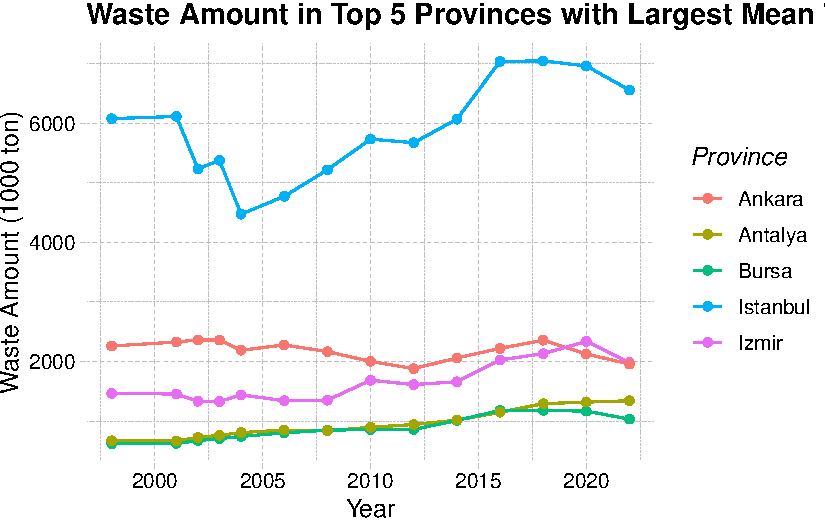
\includegraphics{project_files/figure-pdf/unnamed-chunk-25-1.pdf}

The box plot for the top 10 provinces with the highest average waste
amounts is provided below.

\begin{Shaded}
\begin{Highlighting}[]
\NormalTok{top10\_summary }\OtherTok{\textless{}{-}}\NormalTok{ ts\_province }\SpecialCharTok{\%\textgreater{}\%}
  \FunctionTok{group\_by}\NormalTok{(Province) }\SpecialCharTok{\%\textgreater{}\%}
  \FunctionTok{summarise}\NormalTok{(}\AttributeTok{mean\_waste =} \FunctionTok{mean}\NormalTok{(}\StringTok{\textasciigrave{}}\AttributeTok{Waste amount (1000 ton)}\StringTok{\textasciigrave{}}\NormalTok{, }\AttributeTok{na.rm =} \ConstantTok{TRUE}\NormalTok{)) }\SpecialCharTok{\%\textgreater{}\%}
  \FunctionTok{arrange}\NormalTok{(}\FunctionTok{desc}\NormalTok{(mean\_waste)) }\SpecialCharTok{\%\textgreater{}\%}
  \FunctionTok{top\_n}\NormalTok{(}\DecValTok{10}\NormalTok{, mean\_waste)}

\NormalTok{top10\_provinces }\OtherTok{\textless{}{-}}\NormalTok{ top10\_summary}\SpecialCharTok{$}\NormalTok{Province}
\NormalTok{top10\_data }\OtherTok{\textless{}{-}}\NormalTok{ ts\_province }\SpecialCharTok{\%\textgreater{}\%}
  \FunctionTok{filter}\NormalTok{(Province }\SpecialCharTok{\%in\%}\NormalTok{ top10\_provinces)}

\NormalTok{top10\_data }\OtherTok{\textless{}{-}}\NormalTok{ top10\_data }\SpecialCharTok{\%\textgreater{}\%}
  \FunctionTok{mutate}\NormalTok{(}\AttributeTok{Province =} \FunctionTok{factor}\NormalTok{(Province, }\AttributeTok{levels =}\NormalTok{ top10\_summary}\SpecialCharTok{$}\NormalTok{Province[}\FunctionTok{order}\NormalTok{(top10\_summary}\SpecialCharTok{$}\NormalTok{mean\_waste)]))}

\FunctionTok{ggplot}\NormalTok{(top10\_data, }\FunctionTok{aes}\NormalTok{(}\AttributeTok{x =}\NormalTok{ Province, }\AttributeTok{y =} \StringTok{\textasciigrave{}}\AttributeTok{Waste amount (1000 ton)}\StringTok{\textasciigrave{}}\NormalTok{, }\AttributeTok{fill =}\NormalTok{ Province)) }\SpecialCharTok{+}
  \FunctionTok{geom\_boxplot}\NormalTok{() }\SpecialCharTok{+}
  \FunctionTok{labs}\NormalTok{(}\AttributeTok{title =} \StringTok{"Waste Amounts by Province (Top 10 Provinces)"}\NormalTok{,}
       \AttributeTok{x =} \StringTok{"Province"}\NormalTok{,}
       \AttributeTok{y =} \StringTok{"Waste Amount (1000 ton)"}\NormalTok{) }\SpecialCharTok{+}
  \FunctionTok{theme\_minimal}\NormalTok{() }\SpecialCharTok{+}
  \FunctionTok{theme}\NormalTok{(}\AttributeTok{axis.text.x =} \FunctionTok{element\_text}\NormalTok{(}\AttributeTok{angle =} \DecValTok{90}\NormalTok{, }\AttributeTok{hjust =} \DecValTok{1}\NormalTok{))}
\end{Highlighting}
\end{Shaded}

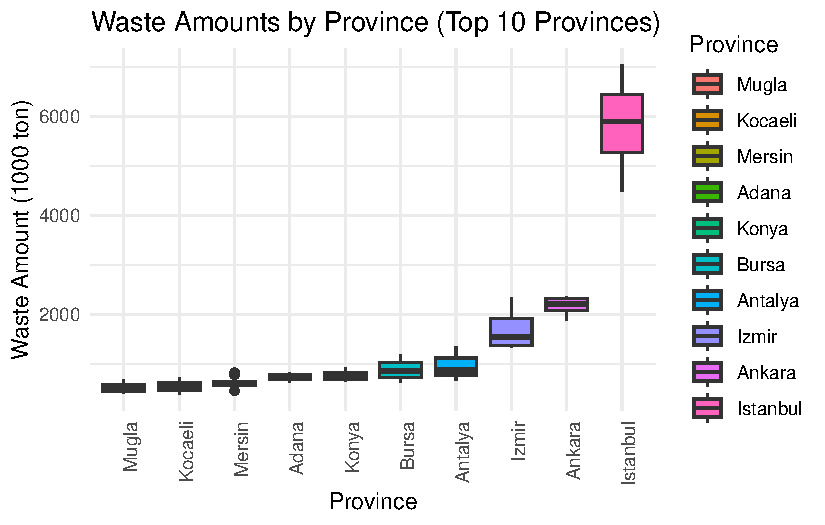
\includegraphics{project_files/figure-pdf/unnamed-chunk-26-1.pdf}

When İstanbul, which was very dominant in the previous boxplot, is
excluded, the results are also examined.

\begin{Shaded}
\begin{Highlighting}[]
\NormalTok{ts\_province\_no\_istanbul }\OtherTok{\textless{}{-}}\NormalTok{ ts\_province }\SpecialCharTok{\%\textgreater{}\%} \FunctionTok{filter}\NormalTok{(Province }\SpecialCharTok{!=} \StringTok{"İstanbul"}\NormalTok{)}
\NormalTok{top10\_summary\_no\_istanbul }\OtherTok{\textless{}{-}}\NormalTok{ ts\_province\_no\_istanbul }\SpecialCharTok{\%\textgreater{}\%}
  \FunctionTok{group\_by}\NormalTok{(Province) }\SpecialCharTok{\%\textgreater{}\%}
  \FunctionTok{summarise}\NormalTok{(}\AttributeTok{mean\_waste =} \FunctionTok{mean}\NormalTok{(}\StringTok{\textasciigrave{}}\AttributeTok{Waste amount (1000 ton)}\StringTok{\textasciigrave{}}\NormalTok{, }\AttributeTok{na.rm =} \ConstantTok{TRUE}\NormalTok{)) }\SpecialCharTok{\%\textgreater{}\%}
  \FunctionTok{arrange}\NormalTok{(}\FunctionTok{desc}\NormalTok{(mean\_waste)) }\SpecialCharTok{\%\textgreater{}\%}
  \FunctionTok{top\_n}\NormalTok{(}\DecValTok{10}\NormalTok{, mean\_waste)}

\NormalTok{top10\_provinces\_no\_istanbul }\OtherTok{\textless{}{-}}\NormalTok{ top10\_summary\_no\_istanbul}\SpecialCharTok{$}\NormalTok{Province}
\NormalTok{top10\_data\_no\_istanbul }\OtherTok{\textless{}{-}}\NormalTok{ ts\_province\_no\_istanbul }\SpecialCharTok{\%\textgreater{}\%}
  \FunctionTok{filter}\NormalTok{(Province }\SpecialCharTok{\%in\%}\NormalTok{ top10\_provinces\_no\_istanbul)}

\NormalTok{top10\_data\_no\_istanbul }\OtherTok{\textless{}{-}}\NormalTok{ top10\_data\_no\_istanbul }\SpecialCharTok{\%\textgreater{}\%}
  \FunctionTok{mutate}\NormalTok{(}\AttributeTok{Province =} \FunctionTok{factor}\NormalTok{(Province, }\AttributeTok{levels =}\NormalTok{ top10\_summary\_no\_istanbul}\SpecialCharTok{$}\NormalTok{Province[}\FunctionTok{order}\NormalTok{(top10\_summary\_no\_istanbul}\SpecialCharTok{$}\NormalTok{mean\_waste)]))}

\FunctionTok{ggplot}\NormalTok{(top10\_data\_no\_istanbul, }\FunctionTok{aes}\NormalTok{(}\AttributeTok{x =}\NormalTok{ Province, }\AttributeTok{y =} \StringTok{\textasciigrave{}}\AttributeTok{Waste amount (1000 ton)}\StringTok{\textasciigrave{}}\NormalTok{, }\AttributeTok{fill =}\NormalTok{ Province)) }\SpecialCharTok{+}
  \FunctionTok{geom\_boxplot}\NormalTok{() }\SpecialCharTok{+}
  \FunctionTok{labs}\NormalTok{(}\AttributeTok{title =} \StringTok{"Waste Amounts by Province (Top 10 Provinces, Excluding İstanbul)"}\NormalTok{,}
       \AttributeTok{x =} \StringTok{"Province"}\NormalTok{,}
       \AttributeTok{y =} \StringTok{"Waste Amount (1000 ton)"}\NormalTok{) }\SpecialCharTok{+}
  \FunctionTok{theme\_minimal}\NormalTok{() }\SpecialCharTok{+}
  \FunctionTok{theme}\NormalTok{(}\AttributeTok{axis.text.x =} \FunctionTok{element\_text}\NormalTok{(}\AttributeTok{angle =} \DecValTok{90}\NormalTok{, }\AttributeTok{hjust =} \DecValTok{1}\NormalTok{))}
\end{Highlighting}
\end{Shaded}

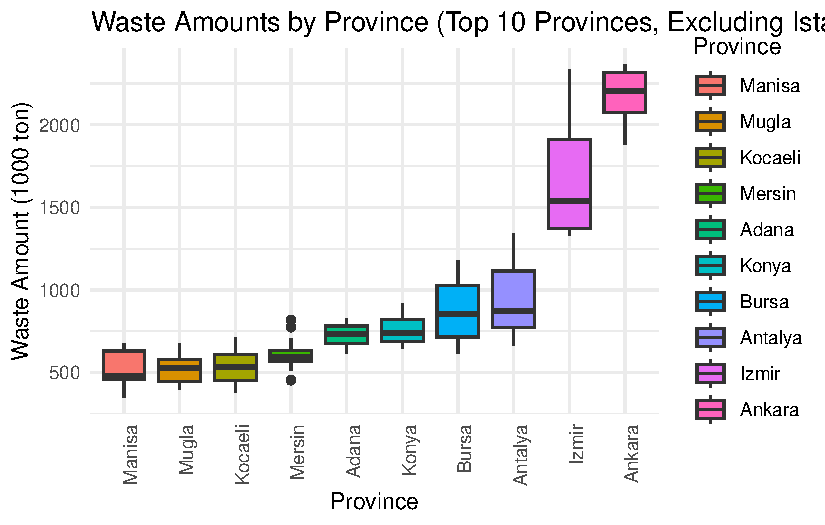
\includegraphics{project_files/figure-pdf/unnamed-chunk-27-1.pdf}

\subsection[{3.2 Regression Analysis} ]{\texorpdfstring{{3.2 Regression
Analysis}
\protect
\includegraphics[width=0.27083in,height=0.23958in]{assets/images/tredn.jpg}}{3.2 Regression Analysis }}\label{regression-analysis}

\textbf{\emph{Additional Data}}

The data sets needed to identify variables contributing to total waste
generation and to conduct regression analysis have been preprocessed
below.

Data on the {agricultural area} cultivated in the provinces of Turkiye
can be accessed below.

\begin{Shaded}
\begin{Highlighting}[]
\FunctionTok{library}\NormalTok{(openxlsx)}
\FunctionTok{library}\NormalTok{(tidyverse)}
\CommentTok{\# agriculture area}
\NormalTok{agriculture\_area }\OtherTok{\textless{}{-}} \FunctionTok{read.xlsx}\NormalTok{(}\StringTok{"project/data/agriculture\_area.xlsx"}\NormalTok{, }\AttributeTok{colNames =} \ConstantTok{TRUE}\NormalTok{)}
\NormalTok{agriculture\_area }\OtherTok{\textless{}{-}} \FunctionTok{select}\NormalTok{(agriculture\_area, }\SpecialCharTok{{-}}\StringTok{"YIL"}\NormalTok{)  }
\NormalTok{agriculture\_area }\OtherTok{\textless{}{-}} \FunctionTok{select}\NormalTok{(agriculture\_area, }\SpecialCharTok{{-}}\StringTok{"BÖLGE.KODU"}\NormalTok{)  }
\NormalTok{agriculture\_area }\OtherTok{\textless{}{-}} \FunctionTok{rename}\NormalTok{(agriculture\_area, }\StringTok{"Provinces"} \OtherTok{=} \StringTok{"BÖLGE.ADI"}\NormalTok{)}
\NormalTok{agriculture\_area }\OtherTok{\textless{}{-}} \FunctionTok{rename}\NormalTok{(agriculture\_area, }\StringTok{"Agriculture area"} \OtherTok{=}\StringTok{\textasciigrave{}}\AttributeTok{Toplam.işlenen.tarım.alanı.(hektar)}\StringTok{\textasciigrave{}}\NormalTok{)}
\NormalTok{agriculture\_area }\OtherTok{\textless{}{-}}\NormalTok{ agriculture\_area [}\SpecialCharTok{{-}}\FunctionTok{c}\NormalTok{(}\DecValTok{83}\SpecialCharTok{:}\DecValTok{87}\NormalTok{), ]}
\NormalTok{agriculture\_area }\OtherTok{\textless{}{-}}\NormalTok{ agriculture\_area [}\SpecialCharTok{{-}}\FunctionTok{c}\NormalTok{(}\DecValTok{1}\NormalTok{), ]}
\FunctionTok{str}\NormalTok{(agriculture\_area)}
\end{Highlighting}
\end{Shaded}

\begin{verbatim}
'data.frame':   81 obs. of  2 variables:
 $ Provinces       : chr  "İstanbul" "Tekirdağ" "Edirne" "Kırklareli" ...
 $ Agriculture area: num  74041 403706 335499 245224 288589 ...
\end{verbatim}

The data on {educational status} of Turkiye's provinces, categorized by
various levels, is provided in education data set.

\begin{Shaded}
\begin{Highlighting}[]
\CommentTok{\# education}
\NormalTok{education }\OtherTok{\textless{}{-}} \FunctionTok{read.xlsx}\NormalTok{(}\StringTok{"project/data/education.xlsx"}\NormalTok{, }\AttributeTok{colNames =} \ConstantTok{TRUE}\NormalTok{)}
\NormalTok{education }\OtherTok{\textless{}{-}} \FunctionTok{select}\NormalTok{(education, }\SpecialCharTok{{-}}\StringTok{"YIL"}\NormalTok{)  }
\NormalTok{education }\OtherTok{\textless{}{-}} \FunctionTok{select}\NormalTok{(education, }\SpecialCharTok{{-}}\StringTok{"BÖLGE.KODU"}\NormalTok{)}
\NormalTok{education  }\OtherTok{\textless{}{-}} \FunctionTok{rename}\NormalTok{(education , }\StringTok{"Provinces"} \OtherTok{=} \StringTok{"BÖLGE.ADI"}\NormalTok{)}
\NormalTok{education  }\OtherTok{\textless{}{-}} \FunctionTok{rename}\NormalTok{(education , }\StringTok{"Total number of faculty members"} \OtherTok{=} \StringTok{\textasciigrave{}}\AttributeTok{Yükseköğretim.kurumlarında.kendi.biriminde.görevli.öğretim.elemanı.sayısı.:.Toplam.öğretim.elemanı./.Toplam}\StringTok{\textasciigrave{}}\NormalTok{)}
\NormalTok{education  }\OtherTok{\textless{}{-}} \FunctionTok{rename}\NormalTok{(education , }\StringTok{"Total number of illiterate people"} \OtherTok{=} \StringTok{\textasciigrave{}}\AttributeTok{Eğitim.durumuna.göre.nüfus.(15.yaş.ve.üzeri).:.Okuma.yazma.bilmeyen./.Toplam}\StringTok{\textasciigrave{}}\NormalTok{)}
\NormalTok{education  }\OtherTok{\textless{}{-}} \FunctionTok{rename}\NormalTok{(education , }\StringTok{"Number of associate or bachelor\textquotesingle{}s degree graduates"} \OtherTok{=} \StringTok{\textasciigrave{}}\AttributeTok{Yükseköğretim.kurumlarında.önlisans.ve.lisans.düzeyinde.öğrenci.sayıları.:.Mezun./.Toplam}\StringTok{\textasciigrave{}}\NormalTok{)}
\NormalTok{education  }\OtherTok{\textless{}{-}} \FunctionTok{rename}\NormalTok{(education , }\StringTok{"Number of master\textquotesingle{}s degree graduates"} \OtherTok{=} \StringTok{\textasciigrave{}}\AttributeTok{Eğitim.durumuna.göre.nüfus.(15.yaş.ve.üzeri).:.Yüksek.lisans.mezunu./.Toplam}\StringTok{\textasciigrave{}}\NormalTok{)}
\NormalTok{education }\OtherTok{\textless{}{-}}\NormalTok{ education [}\SpecialCharTok{{-}}\FunctionTok{c}\NormalTok{(}\DecValTok{1}\NormalTok{), ]}
\FunctionTok{str}\NormalTok{(education)}
\end{Highlighting}
\end{Shaded}

\begin{verbatim}
'data.frame':   81 obs. of  5 variables:
 $ Provinces                                         : chr  "İstanbul" "Tekirdağ" "Edirne" "Kırklareli" ...
 $ Total number of faculty members                   : num  40140 1221 1871 883 1837 ...
 $ Total number of illiterate people                 : num  206140 11573 7011 4462 17368 ...
 $ Number of associate or bachelor's degree graduates: num  167695 3728 6517 3682 7465 ...
 $ Number of master's degree graduates               : num  389440 14458 6914 5137 18318 ...
\end{verbatim}

The first six rows of the {electricity consumption} data for the
provinces of Turkiye are as follows.

\begin{Shaded}
\begin{Highlighting}[]
\CommentTok{\# electricity consumption}
\NormalTok{electricity\_consumption }\OtherTok{\textless{}{-}} \FunctionTok{read.xlsx}\NormalTok{(}\StringTok{"project/data/electricity\_consumption.xlsx"}\NormalTok{, }\AttributeTok{colNames =} \ConstantTok{TRUE}\NormalTok{)}
\NormalTok{electricity\_consumption }\OtherTok{\textless{}{-}} \FunctionTok{select}\NormalTok{(electricity\_consumption, }\SpecialCharTok{{-}}\StringTok{"YIL"}\NormalTok{)  }
\NormalTok{electricity\_consumption }\OtherTok{\textless{}{-}} \FunctionTok{select}\NormalTok{(electricity\_consumption, }\SpecialCharTok{{-}}\StringTok{"BÖLGE.KODU"}\NormalTok{)  }
\NormalTok{electricity\_consumption  }\OtherTok{\textless{}{-}} \FunctionTok{rename}\NormalTok{(electricity\_consumption , }\StringTok{"Provinces"} \OtherTok{=} \StringTok{"BÖLGE.ADI"}\NormalTok{)}
\NormalTok{electricity\_consumption  }\OtherTok{\textless{}{-}} \FunctionTok{rename}\NormalTok{(electricity\_consumption , }\StringTok{"Total electricity consumption (MWh)"} \OtherTok{=} \StringTok{\textasciigrave{}}\AttributeTok{Toplam.tüketim.(MWh)}\StringTok{\textasciigrave{}}\NormalTok{)}
\NormalTok{electricity\_consumption  }\OtherTok{\textless{}{-}} \FunctionTok{rename}\NormalTok{(electricity\_consumption , }\StringTok{"Electricity consumption per capita (KWh)"} \OtherTok{=} \StringTok{\textasciigrave{}}\AttributeTok{Kişi.başına.toplam.elektrik.tüketimi.(KWh)}\StringTok{\textasciigrave{}}\NormalTok{)}
\NormalTok{electricity\_consumption }\OtherTok{\textless{}{-}}\NormalTok{ electricity\_consumption [}\SpecialCharTok{{-}}\FunctionTok{c}\NormalTok{(}\DecValTok{83}\NormalTok{, }\DecValTok{84}\NormalTok{, }\DecValTok{85}\NormalTok{), ]}
\NormalTok{electricity\_consumption }\OtherTok{\textless{}{-}}\NormalTok{ electricity\_consumption[}\SpecialCharTok{{-}}\FunctionTok{c}\NormalTok{(}\DecValTok{1}\NormalTok{), ]}
\FunctionTok{str}\NormalTok{(electricity\_consumption)}
\end{Highlighting}
\end{Shaded}

\begin{verbatim}
'data.frame':   81 obs. of  3 variables:
 $ Provinces                               : chr  "İstanbul" "Tekirdağ" "Edirne" "Kırklareli" ...
 $ Total electricity consumption (MWh)     : num  41520357 8502879 1299120 2715585 4276586 ...
 $ Electricity consumption per capita (KWh): num  2621 7637 3152 7412 3420 ...
\end{verbatim}

{The GDP} data for the provinces of Turkiye has been obtained.

\begin{Shaded}
\begin{Highlighting}[]
\CommentTok{\# GDP}
\NormalTok{GDP }\OtherTok{\textless{}{-}} \FunctionTok{read.xlsx}\NormalTok{(}\StringTok{"project/data/GDP.xlsx"}\NormalTok{, }\AttributeTok{colNames =} \ConstantTok{TRUE}\NormalTok{)}
\NormalTok{GDP }\OtherTok{\textless{}{-}} \FunctionTok{select}\NormalTok{(GDP, }\SpecialCharTok{{-}}\StringTok{"YIL"}\NormalTok{)  }
\NormalTok{GDP }\OtherTok{\textless{}{-}} \FunctionTok{select}\NormalTok{(GDP, }\SpecialCharTok{{-}}\StringTok{"BÖLGE.KODU"}\NormalTok{)  }
\NormalTok{GDP  }\OtherTok{\textless{}{-}} \FunctionTok{rename}\NormalTok{(GDP , }\StringTok{"Provinces"} \OtherTok{=} \StringTok{"BÖLGE.ADI"}\NormalTok{)}
\NormalTok{GDP  }\OtherTok{\textless{}{-}} \FunctionTok{rename}\NormalTok{(GDP , }\StringTok{"GDP per capita (TL)"} \OtherTok{=} \StringTok{\textasciigrave{}}\AttributeTok{Kişi.başına.GSYH.(TL)}\StringTok{\textasciigrave{}}\NormalTok{)}
\NormalTok{GDP  }\OtherTok{\textless{}{-}} \FunctionTok{rename}\NormalTok{(GDP , }\StringTok{"GDP per capita ($)"} \OtherTok{=} \StringTok{\textasciigrave{}}\AttributeTok{Kişi.başına.GSYH.($)}\StringTok{\textasciigrave{}}\NormalTok{)}
\NormalTok{GDP }\OtherTok{\textless{}{-}}\NormalTok{ GDP [}\SpecialCharTok{{-}}\FunctionTok{c}\NormalTok{(}\DecValTok{83}\NormalTok{, }\DecValTok{84}\NormalTok{), ]}
\FunctionTok{str}\NormalTok{(GDP)}
\end{Highlighting}
\end{Shaded}

\begin{verbatim}
'data.frame':   82 obs. of  3 variables:
 $ Provinces          : chr  "Türkiye" "İstanbul" "Tekirdağ" "Edirne" ...
 $ GDP per capita (TL): num  176651 287524 253501 147752 201355 ...
 $ GDP per capita ($) : num  10659 17349 15296 8915 12150 ...
\end{verbatim}

If the {response variable} is extracted from the municipal data set, the
desired variable of {waste amount} by province can be obtained for the
analysis.

\begin{Shaded}
\begin{Highlighting}[]
\CommentTok{\# Amount of waste}
\NormalTok{response\_variable }\OtherTok{\textless{}{-}} \FunctionTok{select}\NormalTok{(municipal\_waste, }\StringTok{"Provinces"}\NormalTok{)  }
\NormalTok{response\_variable }\OtherTok{\textless{}{-}} \FunctionTok{cbind}\NormalTok{(response\_variable, }\StringTok{"Amount of waste collected (Tonnes)"} \OtherTok{=}\NormalTok{ municipal\_waste}\SpecialCharTok{$}\StringTok{\textasciigrave{}}\AttributeTok{Amount of waste collected (Tonnes) }
\StringTok{\textasciigrave{}}\NormalTok{)}
\FunctionTok{str}\NormalTok{(response\_variable)}
\end{Highlighting}
\end{Shaded}

\begin{verbatim}
'data.frame':   81 obs. of  2 variables:
 $ Provinces                         : chr  "Adana" "Adıyaman" "Afyonkarahisar" "Ağrı" ...
 $ Amount of waste collected (Tonnes): num  665695 179724 198273 181116 111099 ...
\end{verbatim}

{The regression analysis} below has been conducted using the {total
amount of waste collected} at the provincial level as the response
variable. {The independent variables} include {GDP per capita,
agricultural area, total number of faculty members, total number of
illiterate people, number of associate or bachelor's degree graduates,
number of master's degree graduates, and electricity consumption}. The
final table prepared for regression analysis can be found below.

\begin{Shaded}
\begin{Highlighting}[]
\NormalTok{regression\_data }\OtherTok{\textless{}{-}} \FunctionTok{data.frame}\NormalTok{()}
\NormalTok{regression\_data }\OtherTok{\textless{}{-}} \FunctionTok{full\_join}\NormalTok{(response\_variable, agriculture\_area, }\AttributeTok{by =} \StringTok{"Provinces"}\NormalTok{)}
\NormalTok{regression\_data }\OtherTok{\textless{}{-}} \FunctionTok{full\_join}\NormalTok{(regression\_data, education,  }\AttributeTok{by =} \StringTok{"Provinces"}\NormalTok{)}
\NormalTok{regression\_data }\OtherTok{\textless{}{-}} \FunctionTok{full\_join}\NormalTok{(regression\_data, electricity\_consumption,  }\AttributeTok{by =} \StringTok{"Provinces"}\NormalTok{)}
\NormalTok{regression\_data }\OtherTok{\textless{}{-}} \FunctionTok{full\_join}\NormalTok{(regression\_data, GDP,  }\AttributeTok{by =} \StringTok{"Provinces"}\NormalTok{)}
\FunctionTok{str}\NormalTok{(regression\_data)}
\end{Highlighting}
\end{Shaded}

\begin{verbatim}
'data.frame':   82 obs. of  11 variables:
 $ Provinces                                         : chr  "Adana" "Adıyaman" "Afyonkarahisar" "Ağrı" ...
 $ Amount of waste collected (Tonnes)                : num  665695 179724 198273 181116 111099 ...
 $ Agriculture area                                  : num  400819 166921 536127 351566 235758 ...
 $ Total number of faculty members                   : num  2593 925 1647 561 725 ...
 $ Total number of illiterate people                 : num  54962 26688 12334 25954 6815 ...
 $ Number of associate or bachelor's degree graduates: num  7987 2453 6787 2065 2870 ...
 $ Number of master's degree graduates               : num  33810 7359 9331 3925 4385 ...
 $ Total electricity consumption (MWh)               : num  7991581 1327087 2131943 495005 706136 ...
 $ Electricity consumption per capita (KWh)          : num  3531 2099 2865 944 2106 ...
 $ GDP per capita (TL)                               : num  135798 79223 114168 55296 112044 ...
 $ GDP per capita ($)                                : num  8194 4780 6889 3337 6761 ...
\end{verbatim}

\textbf{\emph{Regression Analysis}}

In regression analysis using the forward selection method, the model
begins with the variable that exhibits the highest correlation with the
response variable, `Amount of waste collected'. Subsequently, additional
variables are incorporated into the model based on their partial
correlations.

\begin{Shaded}
\begin{Highlighting}[]
\FunctionTok{library}\NormalTok{(ppcor)}
\end{Highlighting}
\end{Shaded}

\begin{verbatim}
Warning: package 'ppcor' was built under R version 4.3.3
\end{verbatim}

\begin{verbatim}
Zorunlu paket yükleniyor: MASS
\end{verbatim}

\begin{verbatim}

Attaching package: 'MASS'
\end{verbatim}

\begin{verbatim}
The following object is masked from 'package:dplyr':

    select
\end{verbatim}

\begin{Shaded}
\begin{Highlighting}[]
\FunctionTok{library}\NormalTok{(tidyverse)}
\FunctionTok{library}\NormalTok{(readxl)}
\end{Highlighting}
\end{Shaded}

\begin{verbatim}
Warning: package 'readxl' was built under R version 4.3.3
\end{verbatim}

\begin{Shaded}
\begin{Highlighting}[]
\NormalTok{regression\_data }\OtherTok{\textless{}{-}} \FunctionTok{read\_excel}\NormalTok{(}\StringTok{"regression\_data.xlsx"}\NormalTok{)}
\NormalTok{numeric\_cols }\OtherTok{\textless{}{-}} \FunctionTok{c}\NormalTok{(}\StringTok{"Amount of waste collected (Tonnes)"}\NormalTok{, }\StringTok{"Agriculture area"}\NormalTok{, }
                  \StringTok{"Total number of faculty members"}\NormalTok{, }\StringTok{"Total number of illiterate people"}\NormalTok{,}
                  \StringTok{"Number of associate or bachelor\textquotesingle{}s degree graduates"}\NormalTok{, }\StringTok{"Total electricity consumption (MWh)"}\NormalTok{,}
                  \StringTok{"GDP per capita (TL)"}\NormalTok{, }\StringTok{"Number of master\textquotesingle{}s degree graduates"}\NormalTok{)}
\NormalTok{regression\_data[numeric\_cols] }\OtherTok{\textless{}{-}} \FunctionTok{sapply}\NormalTok{(regression\_data[numeric\_cols], as.numeric)}

\ControlFlowTok{if}\NormalTok{(}\FunctionTok{any}\NormalTok{(}\FunctionTok{is.na}\NormalTok{(regression\_data[numeric\_cols]))) \{}
\NormalTok{  regression\_data }\OtherTok{\textless{}{-}} \FunctionTok{na.omit}\NormalTok{(regression\_data)}
\NormalTok{\}}

\NormalTok{constant\_cols }\OtherTok{\textless{}{-}} \FunctionTok{sapply}\NormalTok{(regression\_data[numeric\_cols], }\ControlFlowTok{function}\NormalTok{(x) }\FunctionTok{length}\NormalTok{(}\FunctionTok{unique}\NormalTok{(x)) }\SpecialCharTok{\textless{}=} \DecValTok{1}\NormalTok{)}
\ControlFlowTok{if}\NormalTok{(}\FunctionTok{any}\NormalTok{(constant\_cols)) \{}
\NormalTok{  regression\_data }\OtherTok{\textless{}{-}}\NormalTok{ regression\_data[, }\SpecialCharTok{!}\NormalTok{constant\_cols]}
\NormalTok{\}}

\NormalTok{predictor\_columns }\OtherTok{\textless{}{-}} \FunctionTok{names}\NormalTok{(regression\_data) }\SpecialCharTok{!=} \StringTok{"Amount of waste collected (Tonnes)"}
\NormalTok{correlation }\OtherTok{\textless{}{-}} \FunctionTok{cor}\NormalTok{(regression\_data[predictor\_columns], regression\_data}\SpecialCharTok{$}\StringTok{\textasciigrave{}}\AttributeTok{Amount of waste collected (Tonnes)}\StringTok{\textasciigrave{}}\NormalTok{)}
\FunctionTok{print}\NormalTok{(correlation)}
\end{Highlighting}
\end{Shaded}

\begin{verbatim}
                                                        [,1]
Agriculture area                                   0.1237475
Total number of faculty members                    0.9500715
Total number of illiterate people                  0.8469772
Number of associate or bachelor's degree graduates 0.7395918
Number of master's degree graduates                0.9708360
Total electricity consumption (MWh)                0.9327005
GDP per capita (TL)                                0.5047206
\end{verbatim}

The plot between the response variable and the independent variable with
{highest correlation (Number of master's degree graduates)}:

\begin{Shaded}
\begin{Highlighting}[]
\FunctionTok{library}\NormalTok{(ggthemes)}
\FunctionTok{ggplot}\NormalTok{(regression\_data, }\FunctionTok{aes}\NormalTok{(}\StringTok{\textasciigrave{}}\AttributeTok{Amount of waste collected (Tonnes)}\StringTok{\textasciigrave{}}\SpecialCharTok{/}\DecValTok{10}\SpecialCharTok{\^{}}\DecValTok{4}\NormalTok{,}\StringTok{\textasciigrave{}}\AttributeTok{Number of master\textquotesingle{}s degree graduates}\StringTok{\textasciigrave{}}\SpecialCharTok{/}\DecValTok{10}\SpecialCharTok{\^{}}\DecValTok{4}\NormalTok{)) }\SpecialCharTok{+} \FunctionTok{geom\_point}\NormalTok{(}\AttributeTok{color =} \StringTok{"brown"}\NormalTok{) }\SpecialCharTok{+} \FunctionTok{scale\_x\_log10}\NormalTok{() }\SpecialCharTok{+}
\FunctionTok{scale\_y\_log10}\NormalTok{() }\SpecialCharTok{+} \FunctionTok{theme\_classic}\NormalTok{() }\SpecialCharTok{+} \FunctionTok{labs}\NormalTok{(}\AttributeTok{x =} \StringTok{"The amount of waste collected (kg)"}\NormalTok{, }\AttributeTok{y =} \StringTok{"The number of master\textquotesingle{}s degree graduates (log scale)"}\NormalTok{, }\AttributeTok{title =} \StringTok{"The lineer relationship"}\NormalTok{) }\SpecialCharTok{+} \FunctionTok{coord\_flip}\NormalTok{()}
\end{Highlighting}
\end{Shaded}

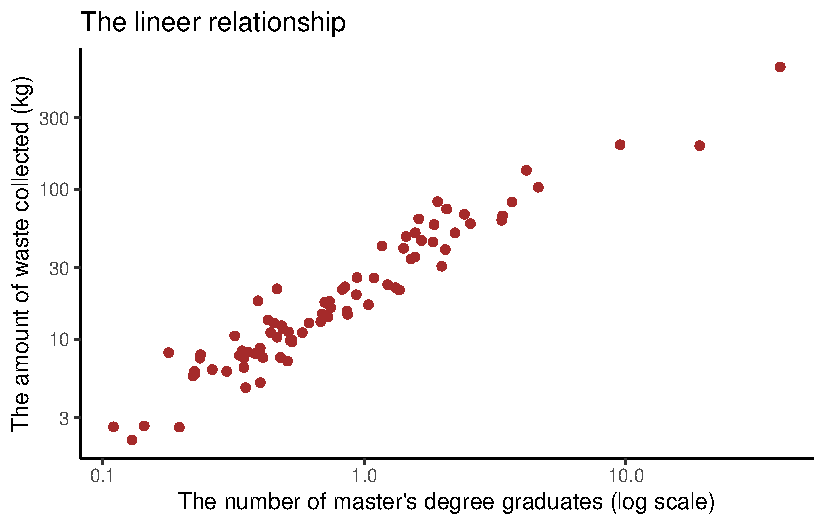
\includegraphics{project_files/figure-pdf/unnamed-chunk-35-1.pdf}

{Partial correlations}: between variables while controlling the variable
with the highest correlation:

\begin{Shaded}
\begin{Highlighting}[]
\FunctionTok{library}\NormalTok{(ppcor)}
\NormalTok{partial\_cor1 }\OtherTok{\textless{}{-}} \FunctionTok{pcor.test}\NormalTok{(regression\_data}\SpecialCharTok{$}\StringTok{\textasciigrave{}}\AttributeTok{Amount of waste collected (Tonnes)}\StringTok{\textasciigrave{}}\NormalTok{, regression\_data}\SpecialCharTok{$}\StringTok{\textasciigrave{}}\AttributeTok{Agriculture area}\StringTok{\textasciigrave{}}\NormalTok{, regression\_data}\SpecialCharTok{$}\StringTok{\textasciigrave{}}\AttributeTok{Number of master\textquotesingle{}s degree graduates}\StringTok{\textasciigrave{}}\NormalTok{)}
\NormalTok{partial\_cor2 }\OtherTok{\textless{}{-}} \FunctionTok{pcor.test}\NormalTok{(regression\_data}\SpecialCharTok{$}\StringTok{\textasciigrave{}}\AttributeTok{Amount of waste collected (Tonnes)}\StringTok{\textasciigrave{}}\NormalTok{, regression\_data}\SpecialCharTok{$}\StringTok{\textasciigrave{}}\AttributeTok{Total number of faculty members}\StringTok{\textasciigrave{}}\NormalTok{, regression\_data}\SpecialCharTok{$}\StringTok{\textasciigrave{}}\AttributeTok{Number of master\textquotesingle{}s degree graduates}\StringTok{\textasciigrave{}}\NormalTok{)}
\NormalTok{partial\_cor3 }\OtherTok{\textless{}{-}}\FunctionTok{pcor.test}\NormalTok{(regression\_data}\SpecialCharTok{$}\StringTok{\textasciigrave{}}\AttributeTok{Amount of waste collected (Tonnes)}\StringTok{\textasciigrave{}}\NormalTok{, regression\_data}\SpecialCharTok{$}\StringTok{\textasciigrave{}}\AttributeTok{Total number of illiterate people}\StringTok{\textasciigrave{}}\NormalTok{, regression\_data}\SpecialCharTok{$}\StringTok{\textasciigrave{}}\AttributeTok{Number of master\textquotesingle{}s degree graduates}\StringTok{\textasciigrave{}}\NormalTok{)}
\NormalTok{partial\_cor4 }\OtherTok{\textless{}{-}}\FunctionTok{pcor.test}\NormalTok{(regression\_data}\SpecialCharTok{$}\StringTok{\textasciigrave{}}\AttributeTok{Amount of waste collected (Tonnes)}\StringTok{\textasciigrave{}}\NormalTok{, regression\_data}\SpecialCharTok{$}\StringTok{\textasciigrave{}}\AttributeTok{Number of associate or bachelor\textquotesingle{}s degree graduates}\StringTok{\textasciigrave{}}\NormalTok{, regression\_data}\SpecialCharTok{$}\StringTok{\textasciigrave{}}\AttributeTok{Number of master\textquotesingle{}s degree graduates}\StringTok{\textasciigrave{}}\NormalTok{)}
\NormalTok{partial\_cor5 }\OtherTok{\textless{}{-}}\FunctionTok{pcor.test}\NormalTok{(regression\_data}\SpecialCharTok{$}\StringTok{\textasciigrave{}}\AttributeTok{Amount of waste collected (Tonnes)}\StringTok{\textasciigrave{}}\NormalTok{, regression\_data}\SpecialCharTok{$}\StringTok{\textasciigrave{}}\AttributeTok{Total electricity consumption (MWh)}\StringTok{\textasciigrave{}}\NormalTok{, regression\_data}\SpecialCharTok{$}\StringTok{\textasciigrave{}}\AttributeTok{Number of master\textquotesingle{}s degree graduates}\StringTok{\textasciigrave{}}\NormalTok{)}
\NormalTok{partial\_cor6 }\OtherTok{\textless{}{-}}\FunctionTok{pcor.test}\NormalTok{(regression\_data}\SpecialCharTok{$}\StringTok{\textasciigrave{}}\AttributeTok{Amount of waste collected (Tonnes)}\StringTok{\textasciigrave{}}\NormalTok{, regression\_data}\SpecialCharTok{$}\StringTok{\textasciigrave{}}\AttributeTok{GDP per capita (TL)}\StringTok{\textasciigrave{}}\NormalTok{, regression\_data}\SpecialCharTok{$}\StringTok{\textasciigrave{}}\AttributeTok{Number of master\textquotesingle{}s degree graduates}\StringTok{\textasciigrave{}}\NormalTok{)}
\FunctionTok{print}\NormalTok{(partial\_cor5)}
\end{Highlighting}
\end{Shaded}

\begin{verbatim}
   estimate      p.value statistic  n gp  Method
1 0.5732279 2.742934e-08  6.178469 81  1 pearson
\end{verbatim}

When examining the partial correlation values for other columns, taking
into account those with significant p-values, {the variable with the
highest partial correlation is `Total electricity consumption'}.
Therefore, it should be the second variable added to the regression
model.

In the next step, partial correlations are examined while controlling
for the two variables with the highest correlations this time. Those
that pass the significant test from the previous step are included in
this calculations.

\begin{Shaded}
\begin{Highlighting}[]
\NormalTok{partial\_corr1 }\OtherTok{\textless{}{-}} \FunctionTok{pcor.test}\NormalTok{(regression\_data}\SpecialCharTok{$}\StringTok{\textasciigrave{}}\AttributeTok{Amount of waste collected (Tonnes)}\StringTok{\textasciigrave{}}\NormalTok{, regression\_data}\SpecialCharTok{$}\StringTok{\textasciigrave{}}\AttributeTok{Total number of faculty members}\StringTok{\textasciigrave{}}\NormalTok{, regression\_data[,}\FunctionTok{c}\NormalTok{(}\DecValTok{6}\NormalTok{,}\DecValTok{7}\NormalTok{)])}
\NormalTok{partial\_corr2 }\OtherTok{\textless{}{-}}\FunctionTok{pcor.test}\NormalTok{(regression\_data}\SpecialCharTok{$}\StringTok{\textasciigrave{}}\AttributeTok{Amount of waste collected (Tonnes)}\StringTok{\textasciigrave{}}\NormalTok{, regression\_data}\SpecialCharTok{$}\StringTok{\textasciigrave{}}\AttributeTok{Total number of illiterate people}\StringTok{\textasciigrave{}}\NormalTok{, regression\_data[,}\FunctionTok{c}\NormalTok{(}\DecValTok{6}\NormalTok{,}\DecValTok{7}\NormalTok{)])}
\FunctionTok{print}\NormalTok{(partial\_corr2)}
\end{Highlighting}
\end{Shaded}

\begin{verbatim}
  estimate     p.value statistic  n gp  Method
1 0.334597 0.002578755  3.115659 81  2 pearson
\end{verbatim}

When the partial correlations calculated by controlling for the two
variables were checked, both were less than 0.5. In other words, there
are no remaining variables with a strong relationship. \textbf{\emph{In
the final model, the independent variables affecting the response
variable ``Amount of waste collected'' were selected as ``Number of
master's degree graduates'' and ``Total electricity consumption'' using
the forward selection method.}}

The results of the multiple regression analysis with the relevant
columns are as follows.

\begin{Shaded}
\begin{Highlighting}[]
\NormalTok{ln\_version\_reg\_data }\OtherTok{\textless{}{-}} \FunctionTok{log10}\NormalTok{(regression\_data)}
\NormalTok{multiple\_regression }\OtherTok{\textless{}{-}} \FunctionTok{lm}\NormalTok{(}\StringTok{\textasciigrave{}}\AttributeTok{Amount of waste collected (Tonnes)}\StringTok{\textasciigrave{}} \SpecialCharTok{\textasciitilde{}} \StringTok{\textasciigrave{}}\AttributeTok{Number of master\textquotesingle{}s degree graduates}\StringTok{\textasciigrave{}} \SpecialCharTok{+} \StringTok{\textasciigrave{}}\AttributeTok{Total electricity consumption (MWh)}\StringTok{\textasciigrave{}}\NormalTok{, }\AttributeTok{data =}\NormalTok{ ln\_version\_reg\_data) }
\FunctionTok{summary}\NormalTok{(multiple\_regression)}
\end{Highlighting}
\end{Shaded}

\begin{verbatim}

Call:
lm(formula = `Amount of waste collected (Tonnes)` ~ `Number of master's degree graduates` + 
    `Total electricity consumption (MWh)`, data = ln_version_reg_data)

Residuals:
     Min       1Q   Median       3Q      Max 
-0.29626 -0.09862 -0.00168  0.07417  0.31978 

Coefficients:
                                      Estimate Std. Error t value Pr(>|t|)    
(Intercept)                            1.26657    0.18717   6.767 2.18e-09 ***
`Number of master's degree graduates`  0.87283    0.07469  11.687  < 2e-16 ***
`Total electricity consumption (MWh)`  0.09492    0.06526   1.455     0.15    
---
Signif. codes:  0 '***' 0.001 '**' 0.01 '*' 0.05 '.' 0.1 ' ' 1

Residual standard error: 0.13 on 78 degrees of freedom
Multiple R-squared:  0.9254,    Adjusted R-squared:  0.9234 
F-statistic: 483.4 on 2 and 78 DF,  p-value: < 2.2e-16
\end{verbatim}

{Since the variable representing total electricity consumption is not
significant, it has been excluded from the model.} Therefore, the most
suitable and effective version of our model, achieving the highest
possible R-squared value, is the simple regression model that solely
includes the variable ``Number of master's graduates''.

\begin{Shaded}
\begin{Highlighting}[]
\NormalTok{regression\_model }\OtherTok{\textless{}{-}} \FunctionTok{lm}\NormalTok{(}\StringTok{\textasciigrave{}}\AttributeTok{Amount of waste collected (Tonnes)}\StringTok{\textasciigrave{}} \SpecialCharTok{\textasciitilde{}} \StringTok{\textasciigrave{}}\AttributeTok{Number of master\textquotesingle{}s degree graduates}\StringTok{\textasciigrave{}}\NormalTok{, }\AttributeTok{data =}\NormalTok{ ln\_version\_reg\_data) }
\FunctionTok{summary}\NormalTok{(regression\_model)}
\end{Highlighting}
\end{Shaded}

\begin{verbatim}

Call:
lm(formula = `Amount of waste collected (Tonnes)` ~ `Number of master's degree graduates`, 
    data = ln_version_reg_data)

Residuals:
      Min        1Q    Median        3Q       Max 
-0.312666 -0.083161 -0.001103  0.064059  0.303947 

Coefficients:
                                      Estimate Std. Error t value Pr(>|t|)    
(Intercept)                             1.4720     0.1237   11.90   <2e-16 ***
`Number of master's degree graduates`   0.9715     0.0315   30.84   <2e-16 ***
---
Signif. codes:  0 '***' 0.001 '**' 0.01 '*' 0.05 '.' 0.1 ' ' 1

Residual standard error: 0.1309 on 79 degrees of freedom
Multiple R-squared:  0.9233,    Adjusted R-squared:  0.9224 
F-statistic: 951.3 on 1 and 79 DF,  p-value: < 2.2e-16
\end{verbatim}

\begin{Shaded}
\begin{Highlighting}[]
\FunctionTok{library}\NormalTok{(broom)}
\FunctionTok{tidy}\NormalTok{(regression\_model)}
\end{Highlighting}
\end{Shaded}

\begin{verbatim}
# A tibble: 2 x 5
  term                                  estimate std.error statistic  p.value
  <chr>                                    <dbl>     <dbl>     <dbl>    <dbl>
1 (Intercept)                              1.47     0.124       11.9 2.68e-19
2 `Number of master's degree graduates`    0.971    0.0315      30.8 8.17e-46
\end{verbatim}

{\textbf{\emph{Model adequacy checking}}} in a regression model is best
achieved by thoroughly analyzing the residuals. Below are the graphs
related to {residual analysis.}

There seems no problem in Residual vs Fitted values plot. This means
that \textbf{\emph{the assumption of constant variance is satisfied.}}

\begin{Shaded}
\begin{Highlighting}[]
\FunctionTok{ggplot}\NormalTok{(ln\_version\_reg\_data, }\FunctionTok{aes}\NormalTok{(}\AttributeTok{x =} \FunctionTok{fitted}\NormalTok{(regression\_model), }\AttributeTok{y =} \FunctionTok{resid}\NormalTok{(regression\_model))) }\SpecialCharTok{+}
  \FunctionTok{geom\_point}\NormalTok{(}\AttributeTok{size =} \DecValTok{3}\NormalTok{, }\AttributeTok{shape =} \DecValTok{18}\NormalTok{) }\SpecialCharTok{+}
  \FunctionTok{geom\_smooth}\NormalTok{(}\AttributeTok{method =} \StringTok{"lm"}\NormalTok{, }\AttributeTok{se =} \ConstantTok{FALSE}\NormalTok{) }\SpecialCharTok{+}
  \FunctionTok{labs}\NormalTok{(}\AttributeTok{x =} \StringTok{"Fitted Values"}\NormalTok{, }\AttributeTok{y =} \StringTok{"Residuals"}\NormalTok{, }\AttributeTok{title =} \StringTok{"Residuals vs Fitted Plot"}\NormalTok{) }\SpecialCharTok{+}
  \FunctionTok{theme\_minimal}\NormalTok{()}
\end{Highlighting}
\end{Shaded}

\begin{verbatim}
`geom_smooth()` using formula = 'y ~ x'
\end{verbatim}

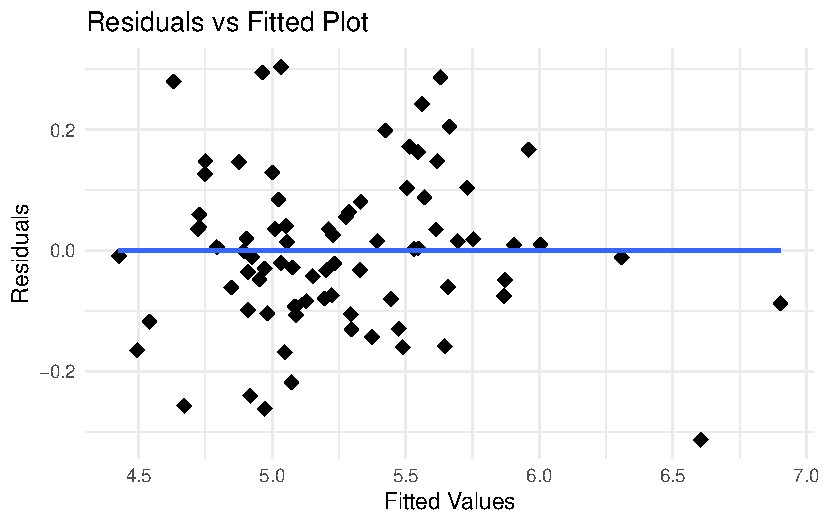
\includegraphics{project_files/figure-pdf/unnamed-chunk-41-1.pdf}

The q-q plot to check if residuals are normally distributed is drawn,
and there is no problem with that.

\begin{Shaded}
\begin{Highlighting}[]
\FunctionTok{library}\NormalTok{(ggthemes)}
\FunctionTok{ggplot}\NormalTok{(ln\_version\_reg\_data, }\FunctionTok{aes}\NormalTok{(}\AttributeTok{sample =} \FunctionTok{resid}\NormalTok{(regression\_model))) }\SpecialCharTok{+}
  \FunctionTok{stat\_qq}\NormalTok{() }\SpecialCharTok{+}
  \FunctionTok{stat\_qq\_line}\NormalTok{(}\AttributeTok{color =} \StringTok{"magenta"}\NormalTok{) }\SpecialCharTok{+}
  \FunctionTok{labs}\NormalTok{(}\AttributeTok{title =} \StringTok{"Normal Q{-}Q Plot"}\NormalTok{) }\SpecialCharTok{+}
  \FunctionTok{theme\_clean}\NormalTok{()}
\end{Highlighting}
\end{Shaded}

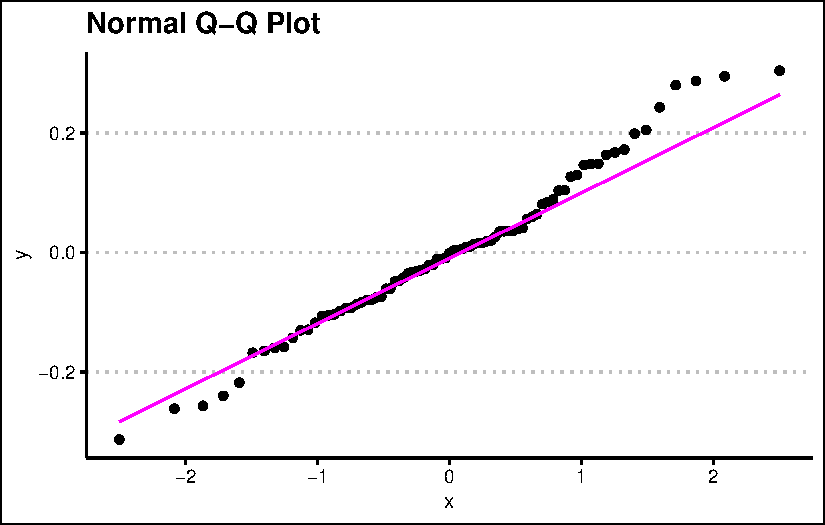
\includegraphics{project_files/figure-pdf/unnamed-chunk-42-1.pdf}

In the Q-Q plot, tails are observed on both the right and left sides. To
be sure, an Anderson-Darling normality test should also be conducted.

\begin{Shaded}
\begin{Highlighting}[]
\FunctionTok{library}\NormalTok{(nortest)}
\NormalTok{residuals }\OtherTok{\textless{}{-}} \FunctionTok{resid}\NormalTok{(regression\_model)}

\NormalTok{ad\_test\_results }\OtherTok{\textless{}{-}} \FunctionTok{ad.test}\NormalTok{(residuals)}
\FunctionTok{print}\NormalTok{(ad\_test\_results)}
\end{Highlighting}
\end{Shaded}

\begin{verbatim}

    Anderson-Darling normality test

data:  residuals
A = 0.43796, p-value = 0.2882
\end{verbatim}

A p-value of 0.28 in the Anderson-Darling test indicates that there is
not enough evidence to reject the null hypothesis that the residuals are
normally distributed. Therefore, it can be assumed that the residuals
are normally distributed; \textbf{\emph{the normality assumption for the
regression model's residuals is considered to be met.}}

The plot below helps to check for \textbf{\emph{homoscedasticity}}.
According to it, \textbf{\emph{there is no such a problem.}}

\begin{Shaded}
\begin{Highlighting}[]
\FunctionTok{ggplot}\NormalTok{(ln\_version\_reg\_data, }\FunctionTok{aes}\NormalTok{(}\AttributeTok{x =} \FunctionTok{fitted}\NormalTok{(regression\_model), }\AttributeTok{y =} \FunctionTok{sqrt}\NormalTok{(}\FunctionTok{abs}\NormalTok{(}\FunctionTok{resid}\NormalTok{(regression\_model))))) }\SpecialCharTok{+}
  \FunctionTok{geom\_point}\NormalTok{(}\AttributeTok{size =} \DecValTok{3}\NormalTok{, }\AttributeTok{color =} \StringTok{"turquoise"}\NormalTok{)  }\SpecialCharTok{+}
  \FunctionTok{labs}\NormalTok{(}\AttributeTok{x =} \StringTok{"Fitted Values"}\NormalTok{, }\AttributeTok{y =} \StringTok{"Square Root of Absolute Residuals"}\NormalTok{, }\AttributeTok{title =} \StringTok{"Scale{-}Location Plot"}\NormalTok{) }\SpecialCharTok{+}
  \FunctionTok{theme\_calc}\NormalTok{()}
\end{Highlighting}
\end{Shaded}

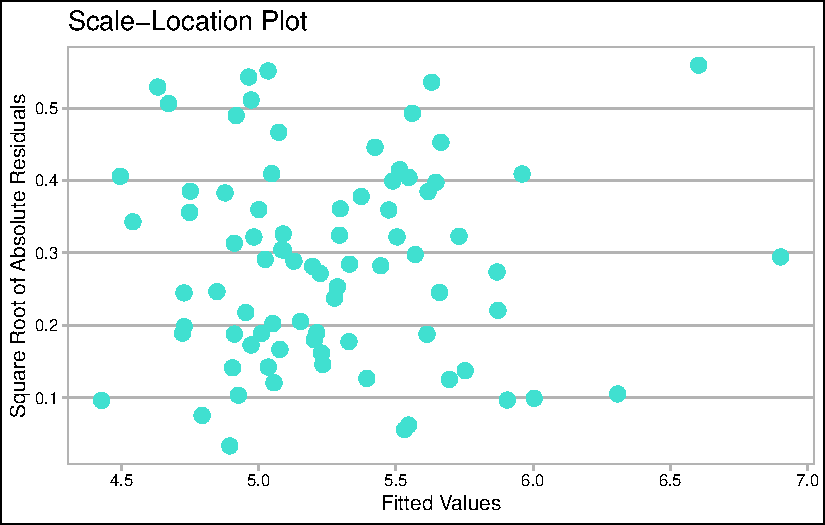
\includegraphics{project_files/figure-pdf/unnamed-chunk-44-1.pdf}

\subsection[{3.3 Time Series Analysis} ]{\texorpdfstring{{3.3 Time
Series Analysis}
\protect
\includegraphics[width=0.375in,height=0.29167in]{assets/images/model.jpg}}{3.3 Time Series Analysis }}\label{time-series-analysis}

The MSW time series data for Turkiye lacks values for some intermediate
years (e.g.~2017, 2019, 2021, etc.), which implies that time series
analysis must be conducted under incomplete information. In this
respect, \textbf{Grey Prediction (GP)} is a powerful forecasting
approach to effectively manage the forecast analysis for MSW {[}6{]}.
This method is particularly advantageous when data availability is
limited, as it requires only a few data points to construct reliable
models {[}6{]}. The core idea of GP involves transforming a complex data
series into a more predictable one using a set of operations, such as
the Accumulated Generating Operator (AGO), the Inverse Accumulating
Operator (IAGO) and Grey Model (GM) {[}6{]}.

The ExoplanetX greyforecasting R package is used to apply grey
prediction models to the MSW time series {[}7{]}. All GP models included
in the package are applied to the data in the background, and the best
model in terms of performance is provided along with its accuracy and
5-year forecasting results.

The GP models in the package are as follows (*):

\begin{enumerate}
\def\labelenumi{\arabic{enumi}.}
\item
  \textbf{gm:} Grey Model (1,1), It's a first-order differential
  equation model with one variable.
\item
  \textbf{gm\_1:} GM(1,1)\_1, This variant of the GM(1,1) model includes
  slight modifications or improvements over the standard GM(1,1) model
  to enhance prediction accuracy or adapt to specific types of data.
\item
  \textbf{gm\_2:} GM(1,1)\_2, Another variant of the GM(1,1) model, with
  different modifications from GM(1,1)\_1, aiming to improve forecasting
  performance under certain conditions.
\item
  \textbf{dgm:} Discrete Grey Model, This model is a discrete version of
  the grey prediction model, which operates on discrete data points
  rather than continuous data, making it suitable for time series data
  that are naturally discrete.
\item
  \textbf{verhulst:} Verhulst Model, The Verhulst model is a nonlinear
  grey prediction model that is particularly useful for data that follow
  an S-shaped growth curve, such as population growth or diffusion
  processes.
\item
  \textbf{pgm:} Grey Power Model, The Grey Power Model is another
  variant of grey models that incorporates power functions into the grey
  modeling process to handle data with certain types of nonlinearity.
\end{enumerate}

First, the necessary packages are installed, and libraries are called.

\begin{Shaded}
\begin{Highlighting}[]
\CommentTok{\# Install and load necessary packages}
\CommentTok{\#install.packages("remotes")}
\CommentTok{\#remotes::install\_github("exoplanetX/greyforecasting")}
\CommentTok{\# install.packages("Metrics")}
\CommentTok{\# install.packages("readxl")}
\CommentTok{\# install.packages("ggplot2")}

\FunctionTok{library}\NormalTok{(greyforecasting)}
\end{Highlighting}
\end{Shaded}

\begin{verbatim}

Attaching package: 'greyforecasting'
\end{verbatim}

\begin{verbatim}
The following object is masked from 'package:dplyr':

    combine
\end{verbatim}

\begin{Shaded}
\begin{Highlighting}[]
\FunctionTok{library}\NormalTok{(Metrics)}
\end{Highlighting}
\end{Shaded}

\begin{verbatim}
Warning: package 'Metrics' was built under R version 4.3.3
\end{verbatim}

\begin{verbatim}

Attaching package: 'Metrics'
\end{verbatim}

\begin{verbatim}
The following objects are masked from 'package:greyforecasting':

    ape, mape
\end{verbatim}

\begin{Shaded}
\begin{Highlighting}[]
\FunctionTok{library}\NormalTok{(readxl)}
\FunctionTok{library}\NormalTok{(tidyverse)}
\end{Highlighting}
\end{Shaded}

When all models are applied to the data in the background, the method
that gives the best result is the \textbf{DGM (Discrete Grey Model)}
method.

\begin{Shaded}
\begin{Highlighting}[]
\NormalTok{file\_path }\OtherTok{\textless{}{-}} \StringTok{"time\_series\_municipal\_waste.xlsx"}
\NormalTok{waste\_data }\OtherTok{\textless{}{-}} \FunctionTok{read\_excel}\NormalTok{(file\_path, }\AttributeTok{sheet =} \StringTok{"Sheet 1"}\NormalTok{)}
\NormalTok{waste\_collected }\OtherTok{\textless{}{-}} \FunctionTok{as.numeric}\NormalTok{(waste\_data[}\DecValTok{3}\NormalTok{, }\SpecialCharTok{{-}}\DecValTok{1}\NormalTok{]) }

\CommentTok{\# AutoML }
\NormalTok{fit\_and\_forecast }\OtherTok{\textless{}{-}} \ControlFlowTok{function}\NormalTok{(model\_func, data, }\AttributeTok{forecast\_steps =} \DecValTok{5}\NormalTok{) \{}
\NormalTok{  model }\OtherTok{\textless{}{-}} \FunctionTok{model\_func}\NormalTok{(data)}
\NormalTok{  fitted\_values }\OtherTok{\textless{}{-}}\NormalTok{ model}\SpecialCharTok{$}\NormalTok{fitted}
\NormalTok{  n }\OtherTok{\textless{}{-}} \FunctionTok{length}\NormalTok{(data)}
\NormalTok{  forecast\_values }\OtherTok{\textless{}{-}} \FunctionTok{numeric}\NormalTok{(forecast\_steps)}
  
  \ControlFlowTok{for}\NormalTok{ (i }\ControlFlowTok{in} \DecValTok{1}\SpecialCharTok{:}\NormalTok{forecast\_steps) \{}
\NormalTok{    extended\_data }\OtherTok{\textless{}{-}} \FunctionTok{c}\NormalTok{(data, forecast\_values[}\DecValTok{1}\SpecialCharTok{:}\NormalTok{(i}\DecValTok{{-}1}\NormalTok{)])}
\NormalTok{    forecast\_model }\OtherTok{\textless{}{-}} \FunctionTok{model\_func}\NormalTok{(extended\_data)}
\NormalTok{    forecast\_values[i] }\OtherTok{\textless{}{-}} \FunctionTok{tail}\NormalTok{(forecast\_model}\SpecialCharTok{$}\NormalTok{fitted, }\DecValTok{1}\NormalTok{)}
\NormalTok{  \}}
  
  \FunctionTok{list}\NormalTok{(}\AttributeTok{model =}\NormalTok{ model, }\AttributeTok{fitted =}\NormalTok{ fitted\_values, }\AttributeTok{forecast =}\NormalTok{ forecast\_values)}
\NormalTok{\}}

\CommentTok{\# Models to evaluate}
\NormalTok{models }\OtherTok{\textless{}{-}} \FunctionTok{list}\NormalTok{(}
  \AttributeTok{gm =}\NormalTok{ gm,}
  \AttributeTok{gm\_1 =}\NormalTok{ gm\_1,}
  \AttributeTok{gm\_2 =}\NormalTok{ gm\_2,}
  \AttributeTok{dgm =}\NormalTok{ dgm,}
  \AttributeTok{verhulst =}\NormalTok{ verhulst,}
  \AttributeTok{pgm =}\NormalTok{ pgm}
\NormalTok{)}

\CommentTok{\# Applying models and calculate accuracy}
\NormalTok{results }\OtherTok{\textless{}{-}} \FunctionTok{lapply}\NormalTok{(models, }\ControlFlowTok{function}\NormalTok{(model\_func) \{}
\NormalTok{  result }\OtherTok{\textless{}{-}} \FunctionTok{fit\_and\_forecast}\NormalTok{(model\_func, waste\_collected, }\AttributeTok{forecast\_steps =} \DecValTok{5}\NormalTok{)}
\NormalTok{  accuracy }\OtherTok{\textless{}{-}} \FunctionTok{rmse}\NormalTok{(waste\_collected[(}\FunctionTok{length}\NormalTok{(waste\_collected)}\SpecialCharTok{{-}}\DecValTok{4}\NormalTok{)}\SpecialCharTok{:}\FunctionTok{length}\NormalTok{(waste\_collected)], result}\SpecialCharTok{$}\NormalTok{forecast)}
  \FunctionTok{list}\NormalTok{(}\AttributeTok{model =}\NormalTok{ result}\SpecialCharTok{$}\NormalTok{model, }\AttributeTok{fitted =}\NormalTok{ result}\SpecialCharTok{$}\NormalTok{fitted, }\AttributeTok{forecast =}\NormalTok{ result}\SpecialCharTok{$}\NormalTok{forecast, }\AttributeTok{accuracy =}\NormalTok{ accuracy)}
\NormalTok{\})}

\NormalTok{best\_model\_index }\OtherTok{\textless{}{-}} \FunctionTok{which.min}\NormalTok{(}\FunctionTok{sapply}\NormalTok{(results, }\ControlFlowTok{function}\NormalTok{(x) x}\SpecialCharTok{$}\NormalTok{accuracy))}
\NormalTok{best\_model\_name }\OtherTok{\textless{}{-}} \FunctionTok{names}\NormalTok{(results)[best\_model\_index]}
\NormalTok{best\_model }\OtherTok{\textless{}{-}}\NormalTok{ results[[best\_model\_index]]}

\FunctionTok{cat}\NormalTok{(}\StringTok{"The best model is:"}\NormalTok{, best\_model\_name, }\StringTok{"}\SpecialCharTok{\textbackslash{}n}\StringTok{"}\NormalTok{)}
\end{Highlighting}
\end{Shaded}

\begin{verbatim}
The best model is: dgm 
\end{verbatim}

Then, the accuracy metric value and forecast values for the next 5 years
are provided for the DGM model.

\begin{Shaded}
\begin{Highlighting}[]
\FunctionTok{cat}\NormalTok{(}\StringTok{"Best model RMSE:"}\NormalTok{, best\_model}\SpecialCharTok{$}\NormalTok{accuracy, }\StringTok{"}\SpecialCharTok{\textbackslash{}n}\StringTok{"}\NormalTok{)}
\end{Highlighting}
\end{Shaded}

\begin{verbatim}
Best model RMSE: 1365.859 
\end{verbatim}

\begin{Shaded}
\begin{Highlighting}[]
\FunctionTok{print}\NormalTok{(best\_model}\SpecialCharTok{$}\NormalTok{forecast)}
\end{Highlighting}
\end{Shaded}

\begin{verbatim}
[1] 30271.09 30922.96 30883.69 31518.20 31456.93
\end{verbatim}

Finally, the original data, fitted values, and forecast points are shown
in the graph below.

\begin{Shaded}
\begin{Highlighting}[]
\NormalTok{years }\OtherTok{\textless{}{-}} \FunctionTok{as.numeric}\NormalTok{(}\FunctionTok{substr}\NormalTok{(}\FunctionTok{names}\NormalTok{(waste\_data)[}\SpecialCharTok{{-}}\DecValTok{1}\NormalTok{], }\DecValTok{1}\NormalTok{, }\DecValTok{4}\NormalTok{))  }
\NormalTok{forecast\_years }\OtherTok{\textless{}{-}}\NormalTok{ (}\FunctionTok{max}\NormalTok{(years) }\SpecialCharTok{+} \DecValTok{1}\NormalTok{)}\SpecialCharTok{:}\NormalTok{(}\FunctionTok{max}\NormalTok{(years) }\SpecialCharTok{+} \FunctionTok{length}\NormalTok{(best\_model}\SpecialCharTok{$}\NormalTok{forecast))}
\NormalTok{plot\_data }\OtherTok{\textless{}{-}} \FunctionTok{data.frame}\NormalTok{(}
  \AttributeTok{Year =} \FunctionTok{c}\NormalTok{(years, forecast\_years),}
  \AttributeTok{Value =} \FunctionTok{c}\NormalTok{(waste\_collected, best\_model}\SpecialCharTok{$}\NormalTok{forecast),}
  \AttributeTok{Type =} \FunctionTok{c}\NormalTok{(}\FunctionTok{rep}\NormalTok{(}\StringTok{"Actual"}\NormalTok{, }\FunctionTok{length}\NormalTok{(waste\_collected)), }\FunctionTok{rep}\NormalTok{(}\StringTok{"Forecast"}\NormalTok{, }\FunctionTok{length}\NormalTok{(best\_model}\SpecialCharTok{$}\NormalTok{forecast)))}
\NormalTok{)}

\NormalTok{fitted\_data }\OtherTok{\textless{}{-}} \FunctionTok{data.frame}\NormalTok{(}
  \AttributeTok{Year =}\NormalTok{ years,}
  \AttributeTok{Value =}\NormalTok{ best\_model}\SpecialCharTok{$}\NormalTok{fitted,}
  \AttributeTok{Type =} \StringTok{"Fitted"}
\NormalTok{)}
\NormalTok{plot\_data }\OtherTok{\textless{}{-}} \FunctionTok{rbind}\NormalTok{(plot\_data, fitted\_data)}

\FunctionTok{ggplot}\NormalTok{(plot\_data, }\FunctionTok{aes}\NormalTok{(}\AttributeTok{x =}\NormalTok{ Year, }\AttributeTok{y =}\NormalTok{ Value, }\AttributeTok{color =}\NormalTok{ Type)) }\SpecialCharTok{+}
  \FunctionTok{geom\_line}\NormalTok{() }\SpecialCharTok{+}
  \FunctionTok{geom\_point}\NormalTok{() }\SpecialCharTok{+}
  \FunctionTok{labs}\NormalTok{(}\AttributeTok{title =} \StringTok{"Grey Model Fitting and Forecast"}\NormalTok{,}
       \AttributeTok{x =} \StringTok{"Year"}\NormalTok{,}
       \AttributeTok{y =} \StringTok{"Amount of Municipal Waste Collected (Thousand tonnes/year)"}\NormalTok{) }\SpecialCharTok{+}
  \FunctionTok{scale\_color\_manual}\NormalTok{(}\AttributeTok{values =} \FunctionTok{c}\NormalTok{(}\StringTok{"Actual"} \OtherTok{=} \StringTok{"green"}\NormalTok{, }\StringTok{"Fitted"} \OtherTok{=} \StringTok{"red"}\NormalTok{, }\StringTok{"Forecast"} \OtherTok{=} \StringTok{"blue"}\NormalTok{)) }\SpecialCharTok{+}
  \FunctionTok{theme\_classic}\NormalTok{()}
\end{Highlighting}
\end{Shaded}

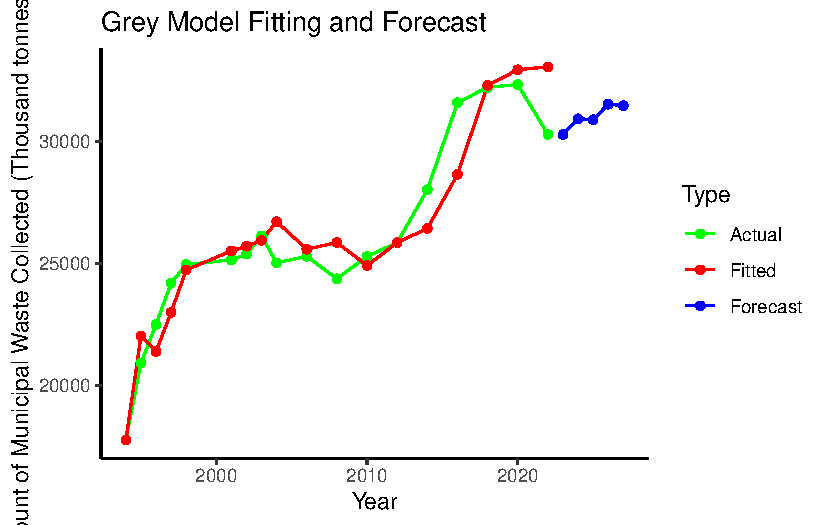
\includegraphics{project_files/figure-pdf/unnamed-chunk-48-1.pdf}

In the above graph, an increasing trend over the years is observed due
to the consideration of total waste amounts. However, Turkiye's
population growth is also a factor that must be taken into account. When
analyzing the per capita waste production instead of the total amounts,
the graph below is obtained.

\begin{Shaded}
\begin{Highlighting}[]
\NormalTok{waste\_collected }\OtherTok{\textless{}{-}} \FunctionTok{as.numeric}\NormalTok{(time\_series\_municipal\_waste[}\DecValTok{4}\NormalTok{, }\SpecialCharTok{{-}}\DecValTok{1}\NormalTok{]) }
\CommentTok{\# AutoML }
\NormalTok{fit\_and\_forecast }\OtherTok{\textless{}{-}} \ControlFlowTok{function}\NormalTok{(model\_func, data, }\AttributeTok{forecast\_steps =} \DecValTok{5}\NormalTok{) \{}
\NormalTok{  model }\OtherTok{\textless{}{-}} \FunctionTok{model\_func}\NormalTok{(data)}
\NormalTok{  fitted\_values }\OtherTok{\textless{}{-}}\NormalTok{ model}\SpecialCharTok{$}\NormalTok{fitted}
\NormalTok{  n }\OtherTok{\textless{}{-}} \FunctionTok{length}\NormalTok{(data)}
\NormalTok{  forecast\_values }\OtherTok{\textless{}{-}} \FunctionTok{numeric}\NormalTok{(forecast\_steps)}
  
  \ControlFlowTok{for}\NormalTok{ (i }\ControlFlowTok{in} \DecValTok{1}\SpecialCharTok{:}\NormalTok{forecast\_steps) \{}
\NormalTok{    extended\_data }\OtherTok{\textless{}{-}} \FunctionTok{c}\NormalTok{(data, forecast\_values[}\DecValTok{1}\SpecialCharTok{:}\NormalTok{(i}\DecValTok{{-}1}\NormalTok{)])}
\NormalTok{    forecast\_model }\OtherTok{\textless{}{-}} \FunctionTok{model\_func}\NormalTok{(extended\_data)}
\NormalTok{    forecast\_values[i] }\OtherTok{\textless{}{-}} \FunctionTok{tail}\NormalTok{(forecast\_model}\SpecialCharTok{$}\NormalTok{fitted, }\DecValTok{1}\NormalTok{)}
\NormalTok{  \}}
  
  \FunctionTok{list}\NormalTok{(}\AttributeTok{model =}\NormalTok{ model, }\AttributeTok{fitted =}\NormalTok{ fitted\_values, }\AttributeTok{forecast =}\NormalTok{ forecast\_values)}
\NormalTok{\}}

\CommentTok{\# Models to evaluate}
\NormalTok{models }\OtherTok{\textless{}{-}} \FunctionTok{list}\NormalTok{(}
  \AttributeTok{gm =}\NormalTok{ gm,}
  \AttributeTok{gm\_1 =}\NormalTok{ gm\_1,}
  \AttributeTok{gm\_2 =}\NormalTok{ gm\_2,}
  \AttributeTok{dgm =}\NormalTok{ dgm,}
  \AttributeTok{verhulst =}\NormalTok{ verhulst,}
  \AttributeTok{pgm =}\NormalTok{ pgm}
\NormalTok{)}

\CommentTok{\# Applying models and calculate accuracy}
\NormalTok{results }\OtherTok{\textless{}{-}} \FunctionTok{lapply}\NormalTok{(models, }\ControlFlowTok{function}\NormalTok{(model\_func) \{}
\NormalTok{  result }\OtherTok{\textless{}{-}} \FunctionTok{fit\_and\_forecast}\NormalTok{(model\_func, waste\_collected, }\AttributeTok{forecast\_steps =} \DecValTok{5}\NormalTok{)}
\NormalTok{  accuracy }\OtherTok{\textless{}{-}} \FunctionTok{rmse}\NormalTok{(waste\_collected[(}\FunctionTok{length}\NormalTok{(waste\_collected)}\SpecialCharTok{{-}}\DecValTok{4}\NormalTok{)}\SpecialCharTok{:}\FunctionTok{length}\NormalTok{(waste\_collected)], result}\SpecialCharTok{$}\NormalTok{forecast)}
  \FunctionTok{list}\NormalTok{(}\AttributeTok{model =}\NormalTok{ result}\SpecialCharTok{$}\NormalTok{model, }\AttributeTok{fitted =}\NormalTok{ result}\SpecialCharTok{$}\NormalTok{fitted, }\AttributeTok{forecast =}\NormalTok{ result}\SpecialCharTok{$}\NormalTok{forecast, }\AttributeTok{accuracy =}\NormalTok{ accuracy)}
\NormalTok{\})}

\NormalTok{best\_model\_index }\OtherTok{\textless{}{-}} \FunctionTok{which.min}\NormalTok{(}\FunctionTok{sapply}\NormalTok{(results, }\ControlFlowTok{function}\NormalTok{(x) x}\SpecialCharTok{$}\NormalTok{accuracy))}
\NormalTok{best\_model\_name }\OtherTok{\textless{}{-}} \FunctionTok{names}\NormalTok{(results)[best\_model\_index]}
\NormalTok{best\_model }\OtherTok{\textless{}{-}}\NormalTok{ results[[best\_model\_index]]}

\FunctionTok{cat}\NormalTok{(}\StringTok{"The best model is:"}\NormalTok{, best\_model\_name, }\StringTok{"}\SpecialCharTok{\textbackslash{}n}\StringTok{"}\NormalTok{)}
\end{Highlighting}
\end{Shaded}

\begin{verbatim}
The best model is: dgm 
\end{verbatim}

Then, the accuracy metric value and forecast values for the next 5 years
are provided for the DGM model.

\begin{Shaded}
\begin{Highlighting}[]
\FunctionTok{cat}\NormalTok{(}\StringTok{"Best model RMSE:"}\NormalTok{, best\_model}\SpecialCharTok{$}\NormalTok{accuracy, }\StringTok{"}\SpecialCharTok{\textbackslash{}n}\StringTok{"}\NormalTok{)}
\end{Highlighting}
\end{Shaded}

\begin{verbatim}
Best model RMSE: 0.1330711 
\end{verbatim}

\begin{Shaded}
\begin{Highlighting}[]
\FunctionTok{print}\NormalTok{(best\_model}\SpecialCharTok{$}\NormalTok{forecast)}
\end{Highlighting}
\end{Shaded}

\begin{verbatim}
[1] 0.9997255 1.0134248 0.9806750 0.9938774 0.9619003
\end{verbatim}

Finally, the original data, fitted values, and forecast points are shown
in the graph below.

\begin{Shaded}
\begin{Highlighting}[]
\NormalTok{years }\OtherTok{\textless{}{-}} \FunctionTok{as.numeric}\NormalTok{(}\FunctionTok{substr}\NormalTok{(}\FunctionTok{names}\NormalTok{(time\_series\_municipal\_waste)[}\SpecialCharTok{{-}}\DecValTok{1}\NormalTok{], }\DecValTok{1}\NormalTok{, }\DecValTok{4}\NormalTok{))  }
\NormalTok{forecast\_years }\OtherTok{\textless{}{-}}\NormalTok{ (}\FunctionTok{max}\NormalTok{(years) }\SpecialCharTok{+} \DecValTok{1}\NormalTok{)}\SpecialCharTok{:}\NormalTok{(}\FunctionTok{max}\NormalTok{(years) }\SpecialCharTok{+} \FunctionTok{length}\NormalTok{(best\_model}\SpecialCharTok{$}\NormalTok{forecast))}
\NormalTok{plot\_data }\OtherTok{\textless{}{-}} \FunctionTok{data.frame}\NormalTok{(}
  \AttributeTok{Year =} \FunctionTok{c}\NormalTok{(years, forecast\_years),}
  \AttributeTok{Value =} \FunctionTok{c}\NormalTok{(waste\_collected, best\_model}\SpecialCharTok{$}\NormalTok{forecast),}
  \AttributeTok{Type =} \FunctionTok{c}\NormalTok{(}\FunctionTok{rep}\NormalTok{(}\StringTok{"Actual"}\NormalTok{, }\FunctionTok{length}\NormalTok{(waste\_collected)), }\FunctionTok{rep}\NormalTok{(}\StringTok{"Forecast"}\NormalTok{, }\FunctionTok{length}\NormalTok{(best\_model}\SpecialCharTok{$}\NormalTok{forecast)))}
\NormalTok{)}

\NormalTok{fitted\_data }\OtherTok{\textless{}{-}} \FunctionTok{data.frame}\NormalTok{(}
  \AttributeTok{Year =}\NormalTok{ years,}
  \AttributeTok{Value =}\NormalTok{ best\_model}\SpecialCharTok{$}\NormalTok{fitted,}
  \AttributeTok{Type =} \StringTok{"Fitted"}
\NormalTok{)}
\NormalTok{plot\_data }\OtherTok{\textless{}{-}} \FunctionTok{rbind}\NormalTok{(plot\_data, fitted\_data)}

\FunctionTok{ggplot}\NormalTok{(plot\_data, }\FunctionTok{aes}\NormalTok{(}\AttributeTok{x =}\NormalTok{ Year, }\AttributeTok{y =}\NormalTok{ Value, }\AttributeTok{color =}\NormalTok{ Type)) }\SpecialCharTok{+}
  \FunctionTok{geom\_line}\NormalTok{() }\SpecialCharTok{+}
  \FunctionTok{geom\_point}\NormalTok{() }\SpecialCharTok{+}
  \FunctionTok{labs}\NormalTok{(}\AttributeTok{title =} \StringTok{"Grey Model Fitting and Forecast"}\NormalTok{,}
       \AttributeTok{x =} \StringTok{"Year"}\NormalTok{,}
       \AttributeTok{y =} \StringTok{"Amount of Municipal Waste Collected (Thousand tonnes/year)"}\NormalTok{) }\SpecialCharTok{+}
  \FunctionTok{scale\_color\_manual}\NormalTok{(}\AttributeTok{values =} \FunctionTok{c}\NormalTok{(}\StringTok{"Actual"} \OtherTok{=} \StringTok{"green"}\NormalTok{, }\StringTok{"Fitted"} \OtherTok{=} \StringTok{"red"}\NormalTok{, }\StringTok{"Forecast"} \OtherTok{=} \StringTok{"blue"}\NormalTok{)) }\SpecialCharTok{+}
  \FunctionTok{theme\_classic}\NormalTok{()}
\end{Highlighting}
\end{Shaded}

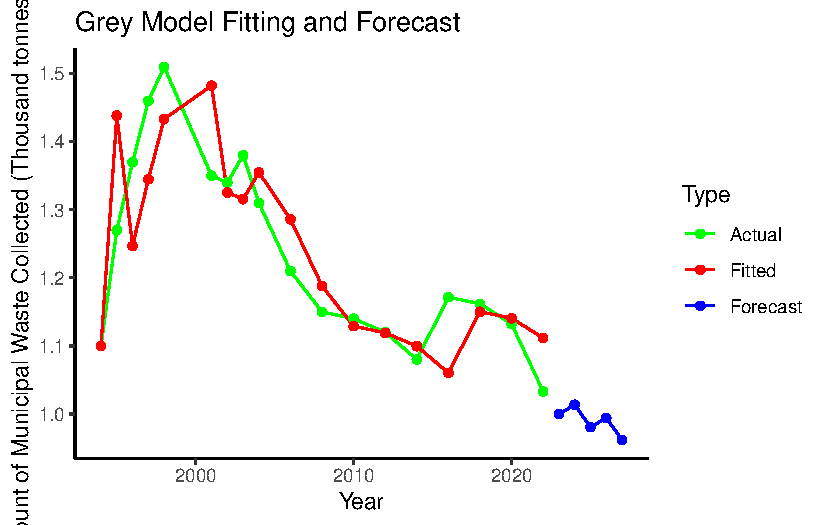
\includegraphics{project_files/figure-pdf/unnamed-chunk-51-1.pdf}

In the waste per capita case, the best fit model according to RMSE is
again the DGM. Unlike before, a decreasing trend over the years is
noticeable in above figure, indicating that the increasing population
must be considered in the analysis.

The following are the results obtained when performing the same grey
forecasting analysis for Ankara.

\begin{Shaded}
\begin{Highlighting}[]
\FunctionTok{library}\NormalTok{(greyforecasting)}
\FunctionTok{library}\NormalTok{(Metrics)}
\FunctionTok{library}\NormalTok{(readxl)}
\FunctionTok{library}\NormalTok{(tidyverse)}
\NormalTok{ankara }\OtherTok{\textless{}{-}}\NormalTok{ ts\_province }\SpecialCharTok{\%\textgreater{}\%} \FunctionTok{filter}\NormalTok{(Province }\SpecialCharTok{==} \StringTok{"Ankara"}\NormalTok{) }\SpecialCharTok{\%\textgreater{}\%} \FunctionTok{arrange}\NormalTok{(Year)}
\NormalTok{ankara\_waste }\OtherTok{\textless{}{-}}\NormalTok{ ankara}\SpecialCharTok{$}\StringTok{\textasciigrave{}}\AttributeTok{Waste amount (1000 ton)}\StringTok{\textasciigrave{}}

\CommentTok{\# AutoML greyforecasting function}
\NormalTok{fit\_and\_forecast }\OtherTok{\textless{}{-}} \ControlFlowTok{function}\NormalTok{(model\_func, data, }\AttributeTok{forecast\_steps =} \DecValTok{5}\NormalTok{) \{}
\NormalTok{  model }\OtherTok{\textless{}{-}} \FunctionTok{model\_func}\NormalTok{(data)}
\NormalTok{  fitted\_values }\OtherTok{\textless{}{-}}\NormalTok{ model}\SpecialCharTok{$}\NormalTok{fitted}
\NormalTok{  forecast\_values }\OtherTok{\textless{}{-}} \FunctionTok{numeric}\NormalTok{(forecast\_steps)}
  
  \ControlFlowTok{for}\NormalTok{ (i }\ControlFlowTok{in} \DecValTok{1}\SpecialCharTok{:}\NormalTok{forecast\_steps) \{}
\NormalTok{    extended\_data }\OtherTok{\textless{}{-}} \FunctionTok{c}\NormalTok{(data, forecast\_values[}\DecValTok{1}\SpecialCharTok{:}\NormalTok{(i}\DecValTok{{-}1}\NormalTok{)])}
\NormalTok{    forecast\_model }\OtherTok{\textless{}{-}} \FunctionTok{model\_func}\NormalTok{(extended\_data)}
\NormalTok{    forecast\_values[i] }\OtherTok{\textless{}{-}} \FunctionTok{tail}\NormalTok{(forecast\_model}\SpecialCharTok{$}\NormalTok{fitted, }\DecValTok{1}\NormalTok{)}
\NormalTok{  \}}
  
  \FunctionTok{list}\NormalTok{(}\AttributeTok{model =}\NormalTok{ model, }\AttributeTok{fitted =}\NormalTok{ fitted\_values, }\AttributeTok{forecast =}\NormalTok{ forecast\_values)}
\NormalTok{\}}

\NormalTok{models }\OtherTok{\textless{}{-}} \FunctionTok{list}\NormalTok{(}
  \AttributeTok{gm =}\NormalTok{ gm,}
  \AttributeTok{gm\_1 =}\NormalTok{ gm\_1,}
  \AttributeTok{gm\_2 =}\NormalTok{ gm\_2,}
  \AttributeTok{dgm =}\NormalTok{ dgm,}
  \AttributeTok{verhulst =}\NormalTok{ verhulst,}
  \AttributeTok{pgm =}\NormalTok{ pgm}
\NormalTok{)}

\NormalTok{results }\OtherTok{\textless{}{-}} \FunctionTok{lapply}\NormalTok{(models, }\ControlFlowTok{function}\NormalTok{(model\_func) \{}
\NormalTok{  result }\OtherTok{\textless{}{-}} \FunctionTok{fit\_and\_forecast}\NormalTok{(model\_func, ankara\_waste, }\AttributeTok{forecast\_steps =} \DecValTok{5}\NormalTok{)}
\NormalTok{  accuracy }\OtherTok{\textless{}{-}} \FunctionTok{rmse}\NormalTok{(}\FunctionTok{tail}\NormalTok{(ankara\_waste, }\FunctionTok{min}\NormalTok{(}\DecValTok{5}\NormalTok{, }\FunctionTok{length}\NormalTok{(ankara\_waste))), result}\SpecialCharTok{$}\NormalTok{forecast)}
  \FunctionTok{list}\NormalTok{(}\AttributeTok{model =}\NormalTok{ result}\SpecialCharTok{$}\NormalTok{model, }\AttributeTok{fitted =}\NormalTok{ result}\SpecialCharTok{$}\NormalTok{fitted, }\AttributeTok{forecast =}\NormalTok{ result}\SpecialCharTok{$}\NormalTok{forecast, }\AttributeTok{accuracy =}\NormalTok{ accuracy)}
\NormalTok{\})}

\NormalTok{best\_model\_index }\OtherTok{\textless{}{-}} \FunctionTok{which.min}\NormalTok{(}\FunctionTok{sapply}\NormalTok{(results, }\ControlFlowTok{function}\NormalTok{(x) x}\SpecialCharTok{$}\NormalTok{accuracy))}
\NormalTok{best\_model\_name }\OtherTok{\textless{}{-}} \FunctionTok{names}\NormalTok{(results)[best\_model\_index]}
\NormalTok{best\_model }\OtherTok{\textless{}{-}}\NormalTok{ results[[best\_model\_index]]}

\FunctionTok{cat}\NormalTok{(}\StringTok{"The best model is:"}\NormalTok{, best\_model\_name, }\StringTok{"}\SpecialCharTok{\textbackslash{}n}\StringTok{"}\NormalTok{)}
\end{Highlighting}
\end{Shaded}

\begin{verbatim}
The best model is: dgm 
\end{verbatim}

\begin{Shaded}
\begin{Highlighting}[]
\FunctionTok{cat}\NormalTok{(}\StringTok{"Best model RMSE:"}\NormalTok{, best\_model}\SpecialCharTok{$}\NormalTok{accuracy, }\StringTok{"}\SpecialCharTok{\textbackslash{}n}\StringTok{"}\NormalTok{)}
\end{Highlighting}
\end{Shaded}

\begin{verbatim}
Best model RMSE: 290.0232 
\end{verbatim}

\begin{Shaded}
\begin{Highlighting}[]
\FunctionTok{print}\NormalTok{(best\_model}\SpecialCharTok{$}\NormalTok{forecast)}
\end{Highlighting}
\end{Shaded}

\begin{verbatim}
[1] 1884.965 1933.066 1861.282 1907.419 1836.855
\end{verbatim}

The graph:

\begin{Shaded}
\begin{Highlighting}[]
\CommentTok{\# Prepare data for plotting}
\NormalTok{years }\OtherTok{\textless{}{-}}\NormalTok{ ankara}\SpecialCharTok{$}\NormalTok{Year}
\NormalTok{forecast\_years }\OtherTok{\textless{}{-}}\NormalTok{ (}\FunctionTok{max}\NormalTok{(years) }\SpecialCharTok{+} \DecValTok{1}\NormalTok{)}\SpecialCharTok{:}\NormalTok{(}\FunctionTok{max}\NormalTok{(years) }\SpecialCharTok{+} \FunctionTok{length}\NormalTok{(best\_model}\SpecialCharTok{$}\NormalTok{forecast))}

\NormalTok{plot\_data }\OtherTok{\textless{}{-}} \FunctionTok{data.frame}\NormalTok{(}
  \AttributeTok{Year =} \FunctionTok{c}\NormalTok{(years, forecast\_years),}
  \AttributeTok{Value =} \FunctionTok{c}\NormalTok{(ankara\_waste, best\_model}\SpecialCharTok{$}\NormalTok{forecast),}
  \AttributeTok{Type =} \FunctionTok{c}\NormalTok{(}\FunctionTok{rep}\NormalTok{(}\StringTok{"Actual"}\NormalTok{, }\FunctionTok{length}\NormalTok{(ankara\_waste)), }\FunctionTok{rep}\NormalTok{(}\StringTok{"Forecast"}\NormalTok{, }\FunctionTok{length}\NormalTok{(best\_model}\SpecialCharTok{$}\NormalTok{forecast)))}
\NormalTok{)}
\NormalTok{fitted\_data }\OtherTok{\textless{}{-}} \FunctionTok{data.frame}\NormalTok{(}
  \AttributeTok{Year =}\NormalTok{ years,}
  \AttributeTok{Value =}\NormalTok{ best\_model}\SpecialCharTok{$}\NormalTok{fitted,}
  \AttributeTok{Type =} \StringTok{"Fitted"}
\NormalTok{)}

\NormalTok{plot\_data }\OtherTok{\textless{}{-}} \FunctionTok{rbind}\NormalTok{(plot\_data, fitted\_data)}

\FunctionTok{ggplot}\NormalTok{(plot\_data, }\FunctionTok{aes}\NormalTok{(}\AttributeTok{x =}\NormalTok{ Year, }\AttributeTok{y =}\NormalTok{ Value, }\AttributeTok{color =}\NormalTok{ Type)) }\SpecialCharTok{+}
  \FunctionTok{geom\_line}\NormalTok{() }\SpecialCharTok{+}
  \FunctionTok{geom\_point}\NormalTok{() }\SpecialCharTok{+}
  \FunctionTok{labs}\NormalTok{(}\AttributeTok{title =} \StringTok{"Grey Model Fitting and Forecast for Ankara"}\NormalTok{,}
       \AttributeTok{x =} \StringTok{"Year"}\NormalTok{,}
       \AttributeTok{y =} \StringTok{"Amount of Municipal Waste Collected (Thousand tonnes/year)"}\NormalTok{) }\SpecialCharTok{+}
  \FunctionTok{scale\_color\_manual}\NormalTok{(}\AttributeTok{values =} \FunctionTok{c}\NormalTok{(}\StringTok{"Actual"} \OtherTok{=} \StringTok{"green"}\NormalTok{, }\StringTok{"Fitted"} \OtherTok{=} \StringTok{"red"}\NormalTok{, }\StringTok{"Forecast"} \OtherTok{=} \StringTok{"blue"}\NormalTok{)) }\SpecialCharTok{+}
  \FunctionTok{theme\_classic}\NormalTok{()}
\end{Highlighting}
\end{Shaded}

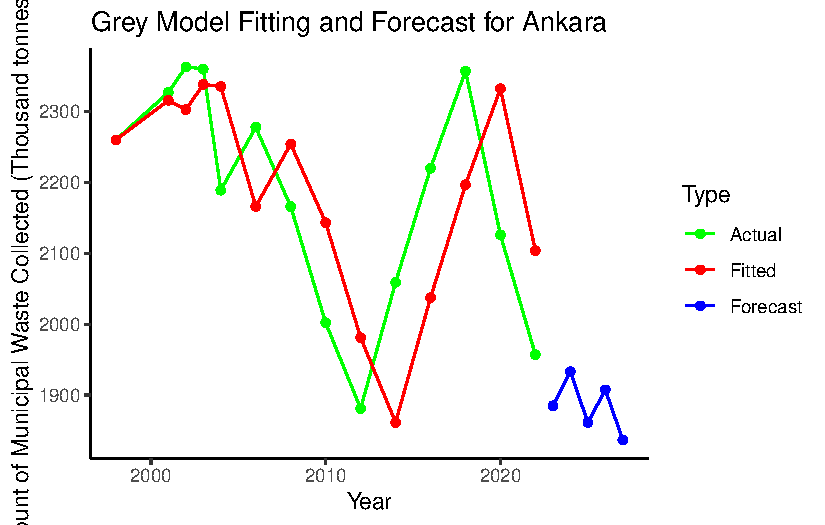
\includegraphics{project_files/figure-pdf/unnamed-chunk-53-1.pdf}

Based on the time series analysis, it was concluded that the DGM model
is the most appropriate time series model for the data containing total
MSW quantities. The fact that data is not available at irregular
intervals of time already tells us that the model suitable for the data
should be discrete. The DGM model forecasted the next five years with
the following values: 30,271.09, 30,922.96, 30,883.69, 31,518.20, and
31,456.93 tonnes. As shown in plots above, the model closely fits the
historical data and strengthens the reliability of these forecast
values. It is also the best method according to the RMSE performance
metric.

The observed increasing trend is consistent with Turkiye's historical
waste generation patterns and highlights the increasing waste management
challenge posed by urbanization and population growth. In addition,
considering Turkiye's population growth, waste generation per capita was
also analysed in the study. The per capita waste forecasts have shown a
decreasing trend over the years.

In addition, the MSW time series analysis of our city (Ankara) is also
included. The DGM model was again dominant, which is logical since it is
again an interval time data.

\section[{4. Conclusion} ]{\texorpdfstring{{4. Conclusion}
\protect
\includegraphics[width=0.28125in,height=\textheight]{assets/images/discussion.png}}{4. Conclusion }}\label{conclusion}

Effective planning of solid waste management systems depends on
analysing and forecasting MSW flows. Accordingly, analysing waste
quantity data is crucial for informed decision-making and strategic
planning related to waste management in Turkiye. In this respect, the
aim of this study is to analyse and forecast municipal solid waste (MSW)
quantities in Turkiye by examining socio-economic factors through
regression analysis and applying time series models for forecasting.

Firstly, EDA was applied to the dataset to reveal the underlying
relationships and patterns in the data. Factors (economic, education,
agriculture, electricity, etc.) that are thought to affect the amount of
waste are added as data and a regression analysis is performed. As a
result, a model using the number of master's degree graduates in
relation to the amount of waste was established and proved to be
accurate.

Then, time series models were evaluated to predict future MSW
quantities. Since the structure of the dataset is discrete with no
regular values in intermediate periods, it was decided that GP methods
are appropriate. Among the GP models, the DGM model was found to be the
most appropriate model for the given data due to its discrete nature and
high accuracy, as indicated by the RMSE performance measure. The
observed upward trend in waste generation is in line with Turkiye's
historical data and emphasizes the increasing challenge of waste
management in urban areas.

Strategic decision-making in waste management systems are crucial to
overcome these challenges. The findings underline the necessity of
sustainable waste management practices and sound policies to reduce the
environmental impacts of increasing waste generation.

\section[{References} ]{\texorpdfstring{{References}
\protect
\includegraphics[width=0.3125in,height=0.30208in]{assets/images/references.jpg}}{References }}\label{references}

\begin{enumerate}
\def\labelenumi{\arabic{enumi}.}
\tightlist
\item
  A. E. İnce, ``Defining New Political Tools for Municipal Solid Waste
  Management of Ankara Metropolitan Municipalitiy After Revision of
  Metropolitan Municipality Law in 2014,'' Master's Thesis, Middle East
  Technical University, Council of Higher Education Thesis Center, 2019.
\item
  TURKSTAT. ``The Results of Address Based Population Registration
  System, 2023.''
  https://data.tuik.gov.tr/Bulten/Index?p=The-Results-of-Address-Based-Population-Registration-System-2023-49684\&dil=2
  (accessed May 5, 2024).
\item
  TURKSTAT. ``Waste Statistics, 2022.''
  https://data.tuik.gov.tr/Bulten/Index?p=Waste-Statistics-2022-49570\&dil=2
  (accessed May 3, 2024).
\item
  OECD. ``Municipal Waste.''
  https://data.oecd.org/waste/municipal-waste.htm (accessed April 21,
  2024).
\item
  H.-W. Chen and N.-B. Chang, ``Prediction analysis of solid waste
  generation based on grey fuzzy dynamic modeling,'' Resources,
  conservation and Recycling, vol.~29, no. 1-2, pp.~1-18, 2000.
\item
  D. Akay and M. Atak, ``Grey prediction with rolling mechanism for
  electricity demand forecasting of Turkey,'' energy, vol.~32, no. 9,
  pp.~1670-1675, 2007.
\item
  ExoplanetX. ``Greyforecasting: A package for grey systems forecasting
  methods.'' https://rdrr.io/github/exoplanetX/greyforecasting/.
  (accessed May 15, 2024).
\end{enumerate}

(*) ChatGPT



\end{document}
